\documentclass[twoside]{book}

% Packages required by doxygen
\usepackage{fixltx2e}
\usepackage{calc}
\usepackage{doxygen}
\usepackage{graphicx}
\usepackage[utf8]{inputenc}
\usepackage{makeidx}
\usepackage{multicol}
\usepackage{multirow}
\PassOptionsToPackage{warn}{textcomp}
\usepackage{textcomp}
\usepackage[nointegrals]{wasysym}
\usepackage[table]{xcolor}

% Font selection
\usepackage[T1]{fontenc}
\usepackage[scaled=.90]{helvet}
\usepackage{courier}
\usepackage{amssymb}
\usepackage{sectsty}
\renewcommand{\familydefault}{\sfdefault}
\allsectionsfont{%
  \fontseries{bc}\selectfont%
  \color{darkgray}%
}
\renewcommand{\DoxyLabelFont}{%
  \fontseries{bc}\selectfont%
  \color{darkgray}%
}
\newcommand{\+}{\discretionary{\mbox{\scriptsize$\hookleftarrow$}}{}{}}

% Page & text layout
\usepackage{geometry}
\geometry{%
  a4paper,%
  top=2.5cm,%
  bottom=2.5cm,%
  left=2.5cm,%
  right=2.5cm%
}
\tolerance=750
\hfuzz=15pt
\hbadness=750
\setlength{\emergencystretch}{15pt}
\setlength{\parindent}{0cm}
\setlength{\parskip}{0.2cm}
\makeatletter
\renewcommand{\paragraph}{%
  \@startsection{paragraph}{4}{0ex}{-1.0ex}{1.0ex}{%
    \normalfont\normalsize\bfseries\SS@parafont%
  }%
}
\renewcommand{\subparagraph}{%
  \@startsection{subparagraph}{5}{0ex}{-1.0ex}{1.0ex}{%
    \normalfont\normalsize\bfseries\SS@subparafont%
  }%
}
\makeatother

% Headers & footers
\usepackage{fancyhdr}
\pagestyle{fancyplain}
\fancyhead[LE]{\fancyplain{}{\bfseries\thepage}}
\fancyhead[CE]{\fancyplain{}{}}
\fancyhead[RE]{\fancyplain{}{\bfseries\leftmark}}
\fancyhead[LO]{\fancyplain{}{\bfseries\rightmark}}
\fancyhead[CO]{\fancyplain{}{}}
\fancyhead[RO]{\fancyplain{}{\bfseries\thepage}}
\fancyfoot[LE]{\fancyplain{}{}}
\fancyfoot[CE]{\fancyplain{}{}}
\fancyfoot[RE]{\fancyplain{}{\bfseries\scriptsize Generated on Wed Mar 9 2016 10\+:52\+:06 for Fuse\+S\+D\+K (i\+O\+S) by Doxygen }}
\fancyfoot[LO]{\fancyplain{}{\bfseries\scriptsize Generated on Wed Mar 9 2016 10\+:52\+:06 for Fuse\+S\+D\+K (i\+O\+S) by Doxygen }}
\fancyfoot[CO]{\fancyplain{}{}}
\fancyfoot[RO]{\fancyplain{}{}}
\renewcommand{\footrulewidth}{0.4pt}
\renewcommand{\chaptermark}[1]{%
  \markboth{#1}{}%
}
\renewcommand{\sectionmark}[1]{%
  \markright{\thesection\ #1}%
}

% Indices & bibliography
\usepackage{natbib}
\usepackage[titles]{tocloft}
\setcounter{tocdepth}{3}
\setcounter{secnumdepth}{5}
\makeindex

% Hyperlinks (required, but should be loaded last)
\usepackage{ifpdf}
\ifpdf
  \usepackage[pdftex,pagebackref=true]{hyperref}
\else
  \usepackage[ps2pdf,pagebackref=true]{hyperref}
\fi
\hypersetup{%
  colorlinks=true,%
  linkcolor=blue,%
  citecolor=blue,%
  unicode%
}

% Custom commands
\newcommand{\clearemptydoublepage}{%
  \newpage{\pagestyle{empty}\cleardoublepage}%
}


%===== C O N T E N T S =====

\begin{document}

% Titlepage & ToC
\hypersetup{pageanchor=false,
             bookmarks=true,
             bookmarksnumbered=true,
             pdfencoding=unicode
            }
\pagenumbering{roman}
\begin{titlepage}
\vspace*{7cm}
\begin{center}%
{\Large Fuse\+S\+D\+K (i\+O\+S) }\\
\vspace*{1cm}
{\large Generated by Doxygen 1.8.8}\\
\vspace*{0.5cm}
{\small Wed Mar 9 2016 10:52:06}\\
\end{center}
\end{titlepage}
\clearemptydoublepage
\tableofcontents
\clearemptydoublepage
\pagenumbering{arabic}
\hypersetup{pageanchor=true}

%--- Begin generated contents ---
\chapter{Deprecated List}
\label{deprecated}
\hypertarget{deprecated}{}

\begin{DoxyRefList}
\item[\label{deprecated__deprecated000002}%
\hypertarget{deprecated__deprecated000002}{}%
Global \hyperlink{interface_fuse_s_d_k_a04c181e3ec49e81ba081a5041df412f6}{\mbox{[}Fuse\+S\+D\+K facebook\+Login\+:\mbox{]}} ]Since \hyperlink{interface_fuse_s_d_k}{Fuse\+S\+D\+K} version 1.\+23. See facebook\+Login\+:\+Name\+:with\+Access\+Token\+: for more information on new method.  
\item[\label{deprecated__deprecated000001}%
\hypertarget{deprecated__deprecated000001}{}%
Global \hyperlink{interface_fuse_s_d_k_aa37c46cc4e49f09fd9b2b40a548b61fc}{\mbox{[}Fuse\+S\+D\+K respond\+To\+Application\+Launch\+Options\+:Application\+:\mbox{]}} ]This method is deprecated and will be removed 
\end{DoxyRefList}
\chapter{Hierarchical Index}
\section{Class Hierarchy}
This inheritance list is sorted roughly, but not completely, alphabetically\+:\begin{DoxyCompactList}
\item $<$N\+S\+Object$>$\begin{DoxyCompactList}
\item \contentsline{section}{$<$Fuse\+Ad\+Delegate$>$}{\pageref{protocol_fuse_ad_delegate-p}}{}
\item \contentsline{section}{Fuse\+A\+P\+I}{\pageref{interface_fuse_a_p_i}}{}
\item \contentsline{section}{$<$Fuse\+Delegate$>$}{\pageref{protocol_fuse_delegate-p}}{}
\item \contentsline{section}{$<$Fuse\+Game\+Data\+Delegate$>$}{\pageref{protocol_fuse_game_data_delegate-p}}{}
\item \contentsline{section}{$<$Fuse\+Overlay\+Delegate$>$}{\pageref{protocol_fuse_overlay_delegate-p}}{}
\end{DoxyCompactList}
\end{DoxyCompactList}

\chapter{Data Structure Index}
\section{Data Structures}
Here are the data structures with brief descriptions\+:\begin{DoxyCompactList}
\item\contentsline{section}{\hyperlink{protocol_fuse_delegate-p}{$<$\+Fuse\+Delegate$>$} \\*This is the Fuse S\+D\+K delegate }{\pageref{protocol_fuse_delegate-p}}{}
\item\contentsline{section}{\hyperlink{interface_fuse_i_a_p_offer_object}{Fuse\+I\+A\+P\+Offer\+Object} \\*Object Returned to the S\+D\+K when a I\+A\+P offer was Accepted, }{\pageref{interface_fuse_i_a_p_offer_object}}{}
\item\contentsline{section}{\hyperlink{interface_fuse_rewarded_object}{Fuse\+Rewarded\+Object} \\*Object Returned to the S\+D\+K when a rewarded Ad was completed, }{\pageref{interface_fuse_rewarded_object}}{}
\item\contentsline{section}{\hyperlink{interface_fuse_s_d_k}{Fuse\+S\+D\+K} \\*This is the main Fuse S\+D\+K static class }{\pageref{interface_fuse_s_d_k}}{}
\item\contentsline{section}{\hyperlink{interface_fuse_virtual_goods_offer_object}{Fuse\+Virtual\+Goods\+Offer\+Object} \\*Object Returned to the S\+D\+K when a Virtual Goods offer was Accepted, }{\pageref{interface_fuse_virtual_goods_offer_object}}{}
\end{DoxyCompactList}

\chapter{Data Structure Documentation}
\hypertarget{protocol_fuse_delegate-p}{}\section{$<$Fuse\+Delegate$>$ Protocol Reference}
\label{protocol_fuse_delegate-p}\index{$<$\+Fuse\+Delegate$>$@{$<$\+Fuse\+Delegate$>$}}


This is the Fuse S\+D\+K delegate.  




{\ttfamily \#import $<$Fuse\+S\+D\+K.\+h$>$}

Inheritance diagram for $<$Fuse\+Delegate$>$\+:\begin{figure}[H]
\begin{center}
\leavevmode
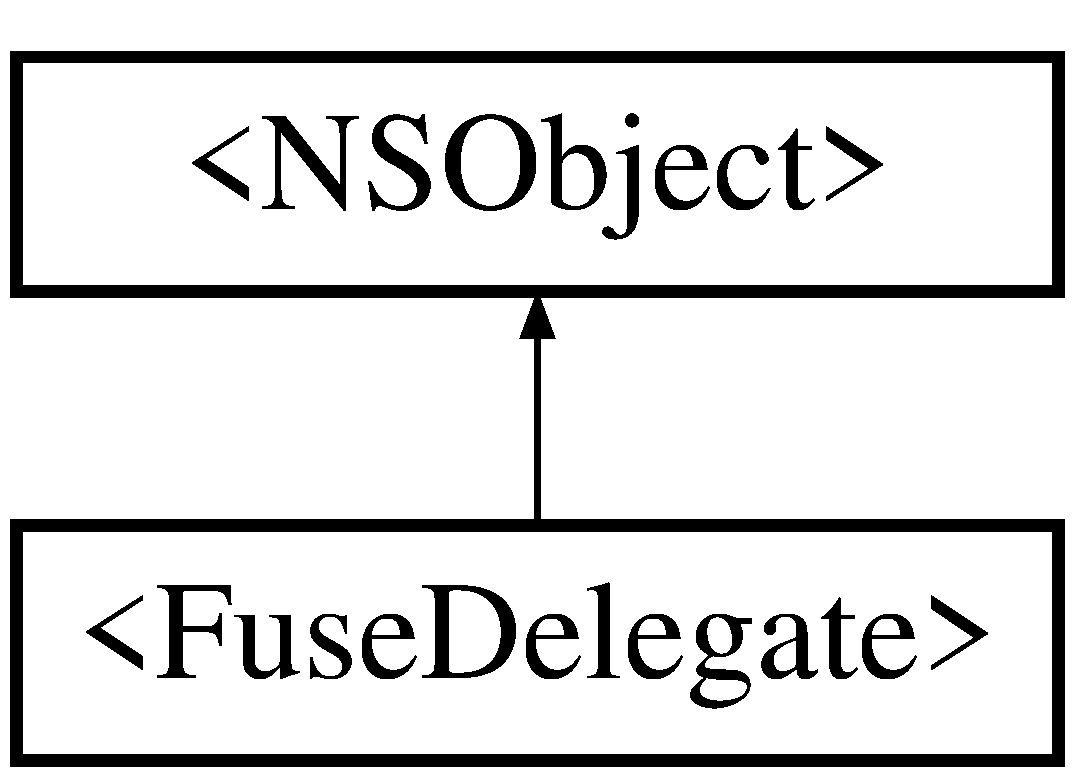
\includegraphics[height=2.000000cm]{protocol_fuse_delegate-p}
\end{center}
\end{figure}
\subsection*{Instance Methods}
\begin{DoxyCompactItemize}
\item 
(void) -\/ \hyperlink{protocol_fuse_delegate-p_a4278f68e73dc20a7a24b331959a1872c}{session\+Start\+Received}
\begin{DoxyCompactList}\small\item\em This method indicates when the server has acknowledged that a session has been established by the client device. \end{DoxyCompactList}\item 
(void) -\/ \hyperlink{protocol_fuse_delegate-p_a24b19ff8cc73955c5cc3b84428b302b0}{session\+Login\+Error\+:}
\begin{DoxyCompactList}\small\item\em This method is invoked when an error has occurred when trying to start a session. \end{DoxyCompactList}\item 
(void) -\/ \hyperlink{protocol_fuse_delegate-p_a85c5468cf940315584698956edcbbdfd}{time\+Updated\+:}
\begin{DoxyCompactList}\small\item\em This method indicates that the server U\+T\+C time has been received by the client device. \end{DoxyCompactList}\item 
(void) -\/ \hyperlink{protocol_fuse_delegate-p_a54a18530604a7ceeb0e9419fc7fa3345}{account\+Login\+Complete\+:\+Account\+:}
\begin{DoxyCompactList}\small\item\em This method notifies the device that an account login request has been received by the server. \end{DoxyCompactList}\item 
(void) -\/ \hyperlink{protocol_fuse_delegate-p_a1c8b10d8ec200c9d2aed94c494109a86}{account\+:login\+Error\+:}
\begin{DoxyCompactList}\small\item\em This method notifies the device that an account login request has failed. \end{DoxyCompactList}\item 
(void) -\/ \hyperlink{protocol_fuse_delegate-p_afc6afbdf6a149756eb2dca5e0fd64b77}{notification\+Action\+:}
\begin{DoxyCompactList}\small\item\em This method indicates that an action should be taken as a result of a notification being closed. \end{DoxyCompactList}\item 
(void) -\/ \hyperlink{protocol_fuse_delegate-p_ac493f7599268adadcc22e7c508b4ba61}{notfication\+Will\+Close}
\begin{DoxyCompactList}\small\item\em This method indicates that a visible notification is being closed. \end{DoxyCompactList}\item 
(void) -\/ \hyperlink{protocol_fuse_delegate-p_a1da152418e0a5dc2c1b108f501c6e627}{game\+Configuration\+Received}
\begin{DoxyCompactList}\small\item\em This method indicates that the game configuration values have been received by the client. \end{DoxyCompactList}\item 
(void) -\/ \hyperlink{protocol_fuse_delegate-p_a5c1b86ecfdc9518f976d5ea96156b408}{friend\+Added\+:\+Error\+:}
\begin{DoxyCompactList}\small\item\em This method indicates the result of an addition of a friend to the Fuse friends list system. \end{DoxyCompactList}\item 
(void) -\/ \hyperlink{protocol_fuse_delegate-p_a94ed7e39378bb2ae24ecc9c941dd0218}{friend\+Removed\+:\+Error\+:}
\begin{DoxyCompactList}\small\item\em This method indicates the result of a removal of a friend to the Fuse friends list system. \end{DoxyCompactList}\item 
(void) -\/ \hyperlink{protocol_fuse_delegate-p_ab48f8ef85f4f32654af102c5fa09c4c1}{friend\+Accepted\+:\+Error\+:}
\begin{DoxyCompactList}\small\item\em This method indicates the result of a acceptance of a friend to the Fuse friends list system. \end{DoxyCompactList}\item 
(void) -\/ \hyperlink{protocol_fuse_delegate-p_a2bc3be54c0a0a4f3cee3e9e96501c5ce}{friend\+Rejected\+:\+Error\+:}
\begin{DoxyCompactList}\small\item\em This method indicates the result of a rejection of a friend to the Fuse friends list system. \end{DoxyCompactList}\item 
(void) -\/ \hyperlink{protocol_fuse_delegate-p_adb2a01d8912d54c4a05a675e10901f6e}{friends\+Migrated\+:\+Error\+:}
\begin{DoxyCompactList}\small\item\em This method indicates the result of a rejection of a request to migrate friends from one account to another. \end{DoxyCompactList}\item 
(void) -\/ \hyperlink{protocol_fuse_delegate-p_a4b29ca96b491f3ac8548a85983aa0cff}{friends\+List\+Updated\+:}
\begin{DoxyCompactList}\small\item\em This method indicates when the friends list on the client has been updated from the server. \end{DoxyCompactList}\item 
(void) -\/ \hyperlink{protocol_fuse_delegate-p_a071433b93b221cbab7c0f112903e4718}{friends\+List\+Error\+:}
\begin{DoxyCompactList}\small\item\em This method indicates when an error has occurred in fetching the friends list from the server. \end{DoxyCompactList}\item 
(void) -\/ \hyperlink{protocol_fuse_delegate-p_a74e3e8647db995888bdf94c64d5ad26b}{purchase\+Verification\+:\+Transaction\+I\+D\+:\+Original\+Transaction\+I\+D\+:}
\begin{DoxyCompactList}\small\item\em This method indicates whether the registered in-\/app purchase has been validated by Apple's servers. \end{DoxyCompactList}\item 
(void) -\/ \hyperlink{protocol_fuse_delegate-p_ad9af5fda0a2199ba2a9a2bafab2f4a82}{ad\+Availability\+Response\+:\+Error\+:}
\begin{DoxyCompactList}\small\item\em Callback response to a request to load for an ad in the Fuse system. \end{DoxyCompactList}\item 
(void) -\/ \hyperlink{protocol_fuse_delegate-p_a3e81f123e745af07c58156c154c13cdc}{rewarded\+Ad\+Complete\+With\+Object\+:}
\begin{DoxyCompactList}\small\item\em Callback to acknowledge a successful rewarded Video Watch. \end{DoxyCompactList}\item 
(void) -\/ \hyperlink{protocol_fuse_delegate-p_ad46a55d7852f92e7615ce5168141bc7a}{I\+A\+P\+Offer\+Accepted\+With\+Object\+:}
\begin{DoxyCompactList}\small\item\em Callback to acknowledge an iap offer was accepted. \end{DoxyCompactList}\item 
(void) -\/ \hyperlink{protocol_fuse_delegate-p_a9577824db67c469466bd720d0193273d}{virtual\+Goods\+Offer\+Accepted\+With\+Object\+:}
\begin{DoxyCompactList}\small\item\em Callback to acknowledge an virtual goods offer was accepted. \end{DoxyCompactList}\item 
(void) -\/ \hyperlink{protocol_fuse_delegate-p_a1513d7db889fcaa54d7248f441b74072}{ad\+Failed\+To\+Display}
\begin{DoxyCompactList}\small\item\em Callback to inform no ad was displayed from show\+Ad\+For\+Zone\+I\+D\+:with\+Options\+: call. \end{DoxyCompactList}\item 
(void) -\/ \hyperlink{protocol_fuse_delegate-p_a2d725902d1f6c4c19d3ce3b65d60052b}{handle\+Ad\+Click\+With\+U\+R\+L\+:}
\begin{DoxyCompactList}\small\item\em If implemented, Ad\+Rally ads will pass this callback including the click-\/through U\+R\+L back to the application. It is then the application's responsibility to present an age gate and continue with the click-\/through if appropriate. \end{DoxyCompactList}\item 
(void) -\/ \hyperlink{protocol_fuse_delegate-p_a88bd02eb971260468ac6f6052bdda28f}{ad\+Did\+Show\+:media\+Type\+:}
\begin{DoxyCompactList}\small\item\em Callback to inform ad Did show. \end{DoxyCompactList}\item 
(void) -\/ \hyperlink{protocol_fuse_delegate-p_aafc293cd46be3bd70eeb60971b961a51}{ad\+Will\+Close}
\begin{DoxyCompactList}\small\item\em Callback to indicates when control is being returned to the application. \end{DoxyCompactList}\end{DoxyCompactItemize}


\subsection{Detailed Description}
This is the Fuse S\+D\+K delegate. 

This delegate is optional. However, relevant information might be passed to an object registered as a \hyperlink{interface_fuse_s_d_k}{Fuse\+S\+D\+K} delegate (application specific). A $<$\hyperlink{protocol_fuse_delegate-p}{Fuse\+Delegate}$>$ is registered in \hyperlink{interface_fuse_s_d_k_adf7ed64a02b9540c9ded4b931ea4e400}{start\+Session\+:delegate\+:with\+Options\+: (\+Fuse\+S\+D\+K)}. 

\subsection{Method Documentation}
\hypertarget{protocol_fuse_delegate-p_a1c8b10d8ec200c9d2aed94c494109a86}{}\index{Fuse\+Delegate-\/p@{Fuse\+Delegate-\/p}!account\+:login\+Error\+:@{account\+:login\+Error\+:}}
\index{account\+:login\+Error\+:@{account\+:login\+Error\+:}!Fuse\+Delegate-\/p@{Fuse\+Delegate-\/p}}
\subsubsection[{account\+:login\+Error\+:}]{\setlength{\rightskip}{0pt plus 5cm}-\/ (void) account\+: 
\begin{DoxyParamCaption}
\item[{(N\+S\+String $\ast$)}]{\+\_\+account\+\_\+id}
\item[{loginError:(N\+S\+Error $\ast$)}]{\+\_\+error}
\end{DoxyParamCaption}
\hspace{0.3cm}{\ttfamily [optional]}}\label{protocol_fuse_delegate-p_a1c8b10d8ec200c9d2aed94c494109a86}


This method notifies the device that an account login request has failed. 

When a user logs in using one of the available \hyperlink{interface_fuse_s_d_k}{Fuse\+S\+D\+K} account method, for instance \hyperlink{interface_fuse_s_d_k_a02a3bc5562d4f6e50bac5339f4ac4046}{game\+Center\+Login\+: (\+Fuse\+S\+D\+K)}, the server will send the client a notification if there is any errors encountered. 
\begin{DoxyParams}{Parameters}
{\em \+\_\+error} & \mbox{[}N\+S\+Error$\ast$\mbox{]} The error value corresponding to a value in E\+Fuse\+Error \\
\hline
{\em \+\_\+account\+\_\+id} & \mbox{[}N\+S\+String$\ast$\mbox{]} The account I\+D of the user attempted to log in \\
\hline
\end{DoxyParams}
\begin{DoxySeeAlso}{See also}
\hyperlink{interface_fuse_s_d_k_a02a3bc5562d4f6e50bac5339f4ac4046}{+ game\+Center\+Login\+: (\+Fuse\+S\+D\+K)} for a sample login method 
\end{DoxySeeAlso}
\begin{DoxySince}{Since}
Fuse S\+D\+K version 1.\+29 
\end{DoxySince}
\hypertarget{protocol_fuse_delegate-p_a54a18530604a7ceeb0e9419fc7fa3345}{}\index{Fuse\+Delegate-\/p@{Fuse\+Delegate-\/p}!account\+Login\+Complete\+:\+Account\+:@{account\+Login\+Complete\+:\+Account\+:}}
\index{account\+Login\+Complete\+:\+Account\+:@{account\+Login\+Complete\+:\+Account\+:}!Fuse\+Delegate-\/p@{Fuse\+Delegate-\/p}}
\subsubsection[{account\+Login\+Complete\+:\+Account\+:}]{\setlength{\rightskip}{0pt plus 5cm}-\/ (void) account\+Login\+Complete\+: 
\begin{DoxyParamCaption}
\item[{(N\+S\+Number $\ast$)}]{\+\_\+type}
\item[{Account:(N\+S\+String $\ast$)}]{\+\_\+account\+\_\+id}
\end{DoxyParamCaption}
\hspace{0.3cm}{\ttfamily [optional]}}\label{protocol_fuse_delegate-p_a54a18530604a7ceeb0e9419fc7fa3345}


This method notifies the device that an account login request has been received by the server. 

When a user logs in using one of the available \hyperlink{interface_fuse_s_d_k}{Fuse\+S\+D\+K} account method, for instance \hyperlink{interface_fuse_s_d_k_a02a3bc5562d4f6e50bac5339f4ac4046}{game\+Center\+Login\+: (\+Fuse\+S\+D\+K)}, the server will send the client a notification once received. This is to prevent any action being taken by the client before this has been received. 
\begin{DoxyParams}{Parameters}
{\em \+\_\+type} & \mbox{[}(N\+S\+Number$\ast$\mbox{]} Account type \\
\hline
{\em \+\_\+account\+\_\+id} & \mbox{[}N\+S\+String$\ast$\mbox{]} The account I\+D of the user logged in \\
\hline
\end{DoxyParams}
\begin{DoxySeeAlso}{See also}
\hyperlink{interface_fuse_s_d_k_a02a3bc5562d4f6e50bac5339f4ac4046}{+ game\+Center\+Login\+: (\+Fuse\+S\+D\+K)} for a sample login method 
\end{DoxySeeAlso}
\hypertarget{protocol_fuse_delegate-p_ad9af5fda0a2199ba2a9a2bafab2f4a82}{}\index{Fuse\+Delegate-\/p@{Fuse\+Delegate-\/p}!ad\+Availability\+Response\+:\+Error\+:@{ad\+Availability\+Response\+:\+Error\+:}}
\index{ad\+Availability\+Response\+:\+Error\+:@{ad\+Availability\+Response\+:\+Error\+:}!Fuse\+Delegate-\/p@{Fuse\+Delegate-\/p}}
\subsubsection[{ad\+Availability\+Response\+:\+Error\+:}]{\setlength{\rightskip}{0pt plus 5cm}-\/ (void) ad\+Availability\+Response\+: 
\begin{DoxyParamCaption}
\item[{(N\+S\+Number $\ast$)}]{\+\_\+available}
\item[{Error:(N\+S\+Error $\ast$)}]{\+\_\+error}
\end{DoxyParamCaption}
\hspace{0.3cm}{\ttfamily [optional]}}\label{protocol_fuse_delegate-p_ad9af5fda0a2199ba2a9a2bafab2f4a82}


Callback response to a request to load for an ad in the Fuse system. 

As a result of the preload\+Ad\+For\+Zone\+I\+D\+: method, this method is invoked when the status of whether an ad is available is known. To handle this response\+:


\begin{DoxyCode}
-(void) adAvailabilityResponse:(NSNumber*)\_available Error:(NSError*)\_error
\{
   BOOL isAvailable = [\_available boolValue];
   \textcolor{keywordtype}{int} error = [\_error code];

   \textcolor{keywordflow}{if} (error != FUSE\_AD\_NO\_ERROR)
   \{
       \textcolor{comment}{// An error has occurred checking for the ad}
   \}
   \textcolor{keywordflow}{else}
   \{
       \textcolor{keywordflow}{if} (isAvailable)
       \{
           \textcolor{comment}{// An ad is available}
       \}
       \textcolor{keywordflow}{else}
       \{
           \textcolor{comment}{// An ad is not available}
       \}
   \}
\}
\end{DoxyCode}



\begin{DoxyParams}{Parameters}
{\em \+\_\+available} & \mbox{[}N\+S\+Error $\ast$\mbox{]} This indicates whether an ad is available (boolean) \\
\hline
{\em \+\_\+error} & \mbox{[}N\+S\+Error $\ast$\mbox{]} This indicates whether an error has occurred and corresponds to values in E\+Fuse\+Error \\
\hline
\end{DoxyParams}
\begin{DoxySeeAlso}{See also}
preload\+Ad\+For\+Zone\+I\+D for more information on how to invoke the process of loading an ad zone. 
\end{DoxySeeAlso}
\begin{DoxySince}{Since}
Fuse S\+D\+K version 1.\+26 
\end{DoxySince}
\hypertarget{protocol_fuse_delegate-p_a88bd02eb971260468ac6f6052bdda28f}{}\index{Fuse\+Delegate-\/p@{Fuse\+Delegate-\/p}!ad\+Did\+Show\+:media\+Type\+:@{ad\+Did\+Show\+:media\+Type\+:}}
\index{ad\+Did\+Show\+:media\+Type\+:@{ad\+Did\+Show\+:media\+Type\+:}!Fuse\+Delegate-\/p@{Fuse\+Delegate-\/p}}
\subsubsection[{ad\+Did\+Show\+:media\+Type\+:}]{\setlength{\rightskip}{0pt plus 5cm}-\/ (void) ad\+Did\+Show\+: 
\begin{DoxyParamCaption}
\item[{(N\+S\+Number $\ast$)}]{\+\_\+network\+I\+D}
\item[{mediaType:(N\+S\+Number $\ast$)}]{\+\_\+media\+Type}
\end{DoxyParamCaption}
\hspace{0.3cm}{\ttfamily [optional]}}\label{protocol_fuse_delegate-p_a88bd02eb971260468ac6f6052bdda28f}


Callback to inform ad Did show. 

\begin{DoxySeeAlso}{See also}
Fuse\+S\+D\+K\+::show\+Ad\+For\+Zone\+I\+D\+:with\+Options\+: 
\end{DoxySeeAlso}
\begin{DoxySince}{Since}
Fuse S\+D\+K version 2.\+2.\+1 
\end{DoxySince}
\hypertarget{protocol_fuse_delegate-p_a1513d7db889fcaa54d7248f441b74072}{}\index{Fuse\+Delegate-\/p@{Fuse\+Delegate-\/p}!ad\+Failed\+To\+Display@{ad\+Failed\+To\+Display}}
\index{ad\+Failed\+To\+Display@{ad\+Failed\+To\+Display}!Fuse\+Delegate-\/p@{Fuse\+Delegate-\/p}}
\subsubsection[{ad\+Failed\+To\+Display}]{\setlength{\rightskip}{0pt plus 5cm}-\/ (void) ad\+Failed\+To\+Display 
\begin{DoxyParamCaption}
{}
\end{DoxyParamCaption}
\hspace{0.3cm}{\ttfamily [optional]}}\label{protocol_fuse_delegate-p_a1513d7db889fcaa54d7248f441b74072}


Callback to inform no ad was displayed from show\+Ad\+For\+Zone\+I\+D\+:with\+Options\+: call. 

\begin{DoxySeeAlso}{See also}
Fshow\+Ad\+For\+Zone\+I\+D\+:with\+Options\+: 
\end{DoxySeeAlso}
\begin{DoxySince}{Since}
Fuse S\+D\+K version 2.\+0.\+0 
\end{DoxySince}
\hypertarget{protocol_fuse_delegate-p_aafc293cd46be3bd70eeb60971b961a51}{}\index{Fuse\+Delegate-\/p@{Fuse\+Delegate-\/p}!ad\+Will\+Close@{ad\+Will\+Close}}
\index{ad\+Will\+Close@{ad\+Will\+Close}!Fuse\+Delegate-\/p@{Fuse\+Delegate-\/p}}
\subsubsection[{ad\+Will\+Close}]{\setlength{\rightskip}{0pt plus 5cm}-\/ (void) ad\+Will\+Close 
\begin{DoxyParamCaption}
{}
\end{DoxyParamCaption}
\hspace{0.3cm}{\ttfamily [required]}}\label{protocol_fuse_delegate-p_aafc293cd46be3bd70eeb60971b961a51}


Callback to indicates when control is being returned to the application. 

When an ad is being dismissed by the user and control is to be returned to the application, this method will be called. Once called, the application can continue execution of the user flow or application. \begin{DoxySeeAlso}{See also}
Fuse\+S\+D\+K\+::show\+Ad\+For\+Zone\+I\+D\+:with\+Options\+: for more information on displaying an ad with a $<$\hyperlink{protocol_fuse_delegate-p}{Fuse\+Delegate}$>$ 
\end{DoxySeeAlso}
\begin{DoxySince}{Since}
\hyperlink{interface_fuse_s_d_k}{Fuse\+S\+D\+K} version 1.\+12 
\end{DoxySince}
\hypertarget{protocol_fuse_delegate-p_ab48f8ef85f4f32654af102c5fa09c4c1}{}\index{Fuse\+Delegate-\/p@{Fuse\+Delegate-\/p}!friend\+Accepted\+:\+Error\+:@{friend\+Accepted\+:\+Error\+:}}
\index{friend\+Accepted\+:\+Error\+:@{friend\+Accepted\+:\+Error\+:}!Fuse\+Delegate-\/p@{Fuse\+Delegate-\/p}}
\subsubsection[{friend\+Accepted\+:\+Error\+:}]{\setlength{\rightskip}{0pt plus 5cm}-\/ (void) friend\+Accepted\+: 
\begin{DoxyParamCaption}
\item[{(N\+S\+String $\ast$)}]{\+\_\+fuse\+\_\+id}
\item[{Error:(N\+S\+Error $\ast$)}]{\+\_\+error}
\end{DoxyParamCaption}
\hspace{0.3cm}{\ttfamily [optional]}}\label{protocol_fuse_delegate-p_ab48f8ef85f4f32654af102c5fa09c4c1}


This method indicates the result of a acceptance of a friend to the Fuse friends list system. 

This method is optional, and only needs to be handled if the application needs to respond to errors in accepting friends. An example implementation would be\+:


\begin{DoxyCode}
-(void) friendAccepted:(NSString*)\_fuse\_id Error:(NSError*)\_error
\{
   \textcolor{keywordflow}{if} ([\_error intValue] == FUSE\_ACCEPT\_FRIEND\_NO\_ERROR)
   \{
       \textcolor{comment}{// no error has occurred in accepting a friend}
   \}
   \textcolor{keywordflow}{else}
   \{
       \textcolor{comment}{// an error has occurred}
   \}
\}
\end{DoxyCode}



\begin{DoxyParams}{Parameters}
{\em \+\_\+fuse\+\_\+id} & \mbox{[}N\+S\+String$\ast$\mbox{]} The fuse I\+D of the account for which the friend was accepted \\
\hline
{\em \+\_\+error} & \mbox{[}int\mbox{]} The error value corresponding to the a value in E\+Fuse\+Error \\
\hline
\end{DoxyParams}
\begin{DoxySeeAlso}{See also}
E\+Fuse\+Error for all possible error codes 

\hyperlink{interface_fuse_s_d_k_ae93cfa17f5b00ab1d28c53a8577c1af0}{+ accept\+Friend\+: (\+Fuse\+S\+D\+K)} for more information on accepting a friend 
\end{DoxySeeAlso}
\begin{DoxySince}{Since}
Fuse S\+D\+K version 1.\+22 
\end{DoxySince}
\hypertarget{protocol_fuse_delegate-p_a5c1b86ecfdc9518f976d5ea96156b408}{}\index{Fuse\+Delegate-\/p@{Fuse\+Delegate-\/p}!friend\+Added\+:\+Error\+:@{friend\+Added\+:\+Error\+:}}
\index{friend\+Added\+:\+Error\+:@{friend\+Added\+:\+Error\+:}!Fuse\+Delegate-\/p@{Fuse\+Delegate-\/p}}
\subsubsection[{friend\+Added\+:\+Error\+:}]{\setlength{\rightskip}{0pt plus 5cm}-\/ (void) friend\+Added\+: 
\begin{DoxyParamCaption}
\item[{(N\+S\+String $\ast$)}]{\+\_\+fuse\+\_\+id}
\item[{Error:(N\+S\+Error $\ast$)}]{\+\_\+error}
\end{DoxyParamCaption}
\hspace{0.3cm}{\ttfamily [optional]}}\label{protocol_fuse_delegate-p_a5c1b86ecfdc9518f976d5ea96156b408}


This method indicates the result of an addition of a friend to the Fuse friends list system. 

This method is optional, and only needs to be handled if the application needs to respond to errors in inviting friends. An example implementation would be\+:


\begin{DoxyCode}
-(void) friendAdded:(NSString*)\_fuse\_id Error:(NSError*)\_error
\{
   \textcolor{keywordflow}{if} (\_error == nil)
   \{
       \textcolor{comment}{// no error has occurred in adding a friend}
   \}
   \textcolor{keywordflow}{else}
   \{
       \textcolor{comment}{// an error has occurred}
   \}
\}
\end{DoxyCode}



\begin{DoxyParams}{Parameters}
{\em \+\_\+fuse\+\_\+id} & \mbox{[}N\+S\+String$\ast$\mbox{]} The fuse I\+D of the account for which the friend was added to \\
\hline
{\em \+\_\+error} & \mbox{[}int\mbox{]} The error value corresponding to the a value in E\+Fuse\+Error \\
\hline
\end{DoxyParams}
\begin{DoxySeeAlso}{See also}
E\+Fuse\+Error for all possible error codes 

\hyperlink{interface_fuse_s_d_k_a92b5888d1e5dafe2ab2a76fda44be4d8}{+ add\+Friend\+: (\+Fuse\+S\+D\+K)} for more information on adding a friend 
\end{DoxySeeAlso}
\begin{DoxySince}{Since}
Fuse S\+D\+K version 1.\+22 
\end{DoxySince}
\hypertarget{protocol_fuse_delegate-p_a2bc3be54c0a0a4f3cee3e9e96501c5ce}{}\index{Fuse\+Delegate-\/p@{Fuse\+Delegate-\/p}!friend\+Rejected\+:\+Error\+:@{friend\+Rejected\+:\+Error\+:}}
\index{friend\+Rejected\+:\+Error\+:@{friend\+Rejected\+:\+Error\+:}!Fuse\+Delegate-\/p@{Fuse\+Delegate-\/p}}
\subsubsection[{friend\+Rejected\+:\+Error\+:}]{\setlength{\rightskip}{0pt plus 5cm}-\/ (void) friend\+Rejected\+: 
\begin{DoxyParamCaption}
\item[{(N\+S\+String $\ast$)}]{\+\_\+fuse\+\_\+id}
\item[{Error:(N\+S\+Error $\ast$)}]{\+\_\+error}
\end{DoxyParamCaption}
\hspace{0.3cm}{\ttfamily [optional]}}\label{protocol_fuse_delegate-p_a2bc3be54c0a0a4f3cee3e9e96501c5ce}


This method indicates the result of a rejection of a friend to the Fuse friends list system. 

This method is optional, and only needs to be handled if the application needs to respond to errors in rejecting friends. An example implementation would be\+:


\begin{DoxyCode}
-(void) friendRejected:(NSString*)\_fuse\_id Error:(NSError*)\_error
\{
   \textcolor{keywordflow}{if} ([\_error intValue] == FUSE\_REJECT\_FRIEND\_NO\_ERROR)
   \{
       \textcolor{comment}{// no error has occurred in accepting a friend}
   \}
   \textcolor{keywordflow}{else}
   \{
       \textcolor{comment}{// an error has occurred}
   \}
\}
\end{DoxyCode}



\begin{DoxyParams}{Parameters}
{\em \+\_\+fuse\+\_\+id} & \mbox{[}N\+S\+String$\ast$\mbox{]} The fuse I\+D of the account for which the friend was rejected \\
\hline
{\em \+\_\+error} & \mbox{[}int\mbox{]} The error value corresponding to the a value in E\+Fuse\+Error \\
\hline
\end{DoxyParams}
\begin{DoxySeeAlso}{See also}
E\+Fuse\+Error for all possible error codes 

\hyperlink{interface_fuse_s_d_k_a8af1416799fd2922db49ed1de406f537}{+ reject\+Friend\+: (\+Fuse\+S\+D\+K)} for more information on rejecting a friend 
\end{DoxySeeAlso}
\begin{DoxySince}{Since}
Fuse S\+D\+K version 1.\+22 
\end{DoxySince}
\hypertarget{protocol_fuse_delegate-p_a94ed7e39378bb2ae24ecc9c941dd0218}{}\index{Fuse\+Delegate-\/p@{Fuse\+Delegate-\/p}!friend\+Removed\+:\+Error\+:@{friend\+Removed\+:\+Error\+:}}
\index{friend\+Removed\+:\+Error\+:@{friend\+Removed\+:\+Error\+:}!Fuse\+Delegate-\/p@{Fuse\+Delegate-\/p}}
\subsubsection[{friend\+Removed\+:\+Error\+:}]{\setlength{\rightskip}{0pt plus 5cm}-\/ (void) friend\+Removed\+: 
\begin{DoxyParamCaption}
\item[{(N\+S\+String $\ast$)}]{\+\_\+fuse\+\_\+id}
\item[{Error:(N\+S\+Error $\ast$)}]{\+\_\+error}
\end{DoxyParamCaption}
\hspace{0.3cm}{\ttfamily [optional]}}\label{protocol_fuse_delegate-p_a94ed7e39378bb2ae24ecc9c941dd0218}


This method indicates the result of a removal of a friend to the Fuse friends list system. 

This method is optional, and only needs to be handled if the application needs to respond to errors in removing friends. An example implementation would be\+:


\begin{DoxyCode}
-(void) friendRemoved:(NSString*)\_fuse\_id Error:(NSError*)\_error
\{
   \textcolor{keywordflow}{if} ([\_error intValue] == FUSE\_REMOVE\_FRIEND\_NO\_ERROR)
   \{
       \textcolor{comment}{// no error has occurred in removing a friend}
   \}
   \textcolor{keywordflow}{else}
   \{
       \textcolor{comment}{// an error has occurred}
   \}
\}
\end{DoxyCode}



\begin{DoxyParams}{Parameters}
{\em \+\_\+fuse\+\_\+id} & \mbox{[}N\+S\+String$\ast$\mbox{]} The fuse I\+D of the account for which the friend was removed \\
\hline
{\em \+\_\+error} & \mbox{[}int\mbox{]} The error value corresponding to the a value in E\+Fuse\+Error \\
\hline
\end{DoxyParams}
\begin{DoxySeeAlso}{See also}
E\+Fuse\+Error for all possible error codes 

\hyperlink{interface_fuse_s_d_k_a1556fd18ab2ae7f062c9d2ebbe2498fc}{+ remove\+Friend\+: (\+Fuse\+S\+D\+K)} for more information on removing a friend 
\end{DoxySeeAlso}
\begin{DoxySince}{Since}
Fuse S\+D\+K version 1.\+22 
\end{DoxySince}
\hypertarget{protocol_fuse_delegate-p_a071433b93b221cbab7c0f112903e4718}{}\index{Fuse\+Delegate-\/p@{Fuse\+Delegate-\/p}!friends\+List\+Error\+:@{friends\+List\+Error\+:}}
\index{friends\+List\+Error\+:@{friends\+List\+Error\+:}!Fuse\+Delegate-\/p@{Fuse\+Delegate-\/p}}
\subsubsection[{friends\+List\+Error\+:}]{\setlength{\rightskip}{0pt plus 5cm}-\/ (void) friends\+List\+Error\+: 
\begin{DoxyParamCaption}
\item[{(N\+S\+Error $\ast$)}]{\+\_\+error}
\end{DoxyParamCaption}
\hspace{0.3cm}{\ttfamily [optional]}}\label{protocol_fuse_delegate-p_a071433b93b221cbab7c0f112903e4718}


This method indicates when an error has occurred in fetching the friends list from the server. 

This method is a result of an error originating from the invocation of \hyperlink{interface_fuse_s_d_k_a11a92658dca5be9d79ca19a66bafb91e}{update\+Friends\+List\+From\+Server (\+Fuse\+S\+D\+K)} and indicates an error has occurred somewhere in the process.


\begin{DoxyCode}
-(void) friendsListError:(NSError*)\_error
\{
   \textcolor{keywordflow}{if} ([\_error intValue] != FUSE\_FRIENDS\_LIST\_NO\_ERROR)
   \{
       \textcolor{comment}{// An error has occurred}
   \}
\}
\end{DoxyCode}



\begin{DoxyParams}{Parameters}
{\em \+\_\+error} & \mbox{[}int\mbox{]} The error value corresponding to the a value in E\+Fuse\+Error \\
\hline
\end{DoxyParams}
\begin{DoxySeeAlso}{See also}
\hyperlink{interface_fuse_s_d_k_a11a92658dca5be9d79ca19a66bafb91e}{+ update\+Friends\+List\+From\+Server (\+Fuse\+S\+D\+K)} or more information on requesting the friends list from the server 
\end{DoxySeeAlso}
\begin{DoxySince}{Since}
Fuse S\+D\+K version 1.\+22 
\end{DoxySince}
\hypertarget{protocol_fuse_delegate-p_a4b29ca96b491f3ac8548a85983aa0cff}{}\index{Fuse\+Delegate-\/p@{Fuse\+Delegate-\/p}!friends\+List\+Updated\+:@{friends\+List\+Updated\+:}}
\index{friends\+List\+Updated\+:@{friends\+List\+Updated\+:}!Fuse\+Delegate-\/p@{Fuse\+Delegate-\/p}}
\subsubsection[{friends\+List\+Updated\+:}]{\setlength{\rightskip}{0pt plus 5cm}-\/ (void) friends\+List\+Updated\+: 
\begin{DoxyParamCaption}
\item[{(N\+S\+Dictionary $\ast$)}]{\+\_\+friends\+List}
\end{DoxyParamCaption}
\hspace{0.3cm}{\ttfamily [optional]}}\label{protocol_fuse_delegate-p_a4b29ca96b491f3ac8548a85983aa0cff}


This method indicates when the friends list on the client has been updated from the server. 

Either on the first fetch or subsequent updates of the friends list, this method is called every time the friends list is updated on the client. A friends list is requested from the server using \hyperlink{interface_fuse_s_d_k_a11a92658dca5be9d79ca19a66bafb91e}{update\+Friends\+List\+From\+Server (\+Fuse\+S\+D\+K)} and the process invokes this method with a dictionary of friends when complete. A sample implementation would be\+:


\begin{DoxyCode}
-(void) friendsListUpdated:(NSDictionary*)\_friendsList
\{
   \textcolor{comment}{// The friends list has returned to the device}

   \textcolor{comment}{// sample code to parse the dictionary}
   NSArray *fuse\_ids = [\_friendsList allKeys];

   \textcolor{keywordflow}{for} (\textcolor{keywordtype}{int} i = 0; i < [fuse\_ids count]; i++)
   \{
       NSString *fuse\_id = [fuse\_ids objectAtIndex:i];

       NSDictionary *friendEntry = (NSDictionary*)[\_friendsList objectForKey:fuse\_id];

       NSLog(\textcolor{stringliteral}{@"Friend is Pending: %d"}, [[friendEntry objectForKey:\textcolor{stringliteral}{@"pending"}] intValue]);
       NSLog(\textcolor{stringliteral}{@"Friend Alias: %@"}, [friendEntry objectForKey:\textcolor{stringliteral}{@"alias"}]);
       NSLog(\textcolor{stringliteral}{@"Friend Fuse ID: %@"}, [friendEntry objectForKey:\textcolor{stringliteral}{@"fuse\_id"}]);
   \}
\}
\end{DoxyCode}



\begin{DoxyParams}{Parameters}
{\em \+\_\+friends\+List} & \\
\hline
\end{DoxyParams}
\begin{DoxySeeAlso}{See also}
\hyperlink{interface_fuse_s_d_k_a11a92658dca5be9d79ca19a66bafb91e}{+ update\+Friends\+List\+From\+Server (\+Fuse\+S\+D\+K)} or more information on requesting the friends list from the server 

\hyperlink{interface_fuse_s_d_k_a31d609ce39be3e6eda04fd32d8036e95}{+ get\+Friends\+List (\+Fuse\+S\+D\+K)} for more information on requesting the local copy of the friends list 

\hyperlink{protocol_fuse_delegate-p_a071433b93b221cbab7c0f112903e4718}{-\/ friends\+List\+Error\+:} to handle errors involved in requesting the friends list from the Fuse server 
\end{DoxySeeAlso}
\begin{DoxySince}{Since}
Fuse S\+D\+K version 1.\+22 
\end{DoxySince}
\hypertarget{protocol_fuse_delegate-p_adb2a01d8912d54c4a05a675e10901f6e}{}\index{Fuse\+Delegate-\/p@{Fuse\+Delegate-\/p}!friends\+Migrated\+:\+Error\+:@{friends\+Migrated\+:\+Error\+:}}
\index{friends\+Migrated\+:\+Error\+:@{friends\+Migrated\+:\+Error\+:}!Fuse\+Delegate-\/p@{Fuse\+Delegate-\/p}}
\subsubsection[{friends\+Migrated\+:\+Error\+:}]{\setlength{\rightskip}{0pt plus 5cm}-\/ (void) friends\+Migrated\+: 
\begin{DoxyParamCaption}
\item[{(N\+S\+String $\ast$)}]{\+\_\+fuse\+\_\+id}
\item[{Error:(N\+S\+Error $\ast$)}]{\+\_\+error}
\end{DoxyParamCaption}
\hspace{0.3cm}{\ttfamily [optional]}}\label{protocol_fuse_delegate-p_adb2a01d8912d54c4a05a675e10901f6e}


This method indicates the result of a rejection of a request to migrate friends from one account to another. 

This method is optional, and only needs to be handled if the application needs to respond to errors in migrating friends. An example implementation would be\+:


\begin{DoxyCode}
-(void) friendsMigrated:(NSString*)\_fuse\_id Error:(NSError*)\_error
\{
    \textcolor{keywordflow}{if} ([\_error intValue] == FUSE\_MIGRATE\_FRIENDS\_NO\_ERROR)
    \{
        \textcolor{comment}{// no error has occurred in accepting a friend}
    \}
    \textcolor{keywordflow}{else}
    \{
        \textcolor{comment}{// an error has occurred}
    \}
\}
\end{DoxyCode}



\begin{DoxyParams}{Parameters}
{\em \+\_\+fuse\+\_\+id} & \mbox{[}N\+S\+String$\ast$\mbox{]} The fuse I\+D of the account for which the friend's are to be migrated from \\
\hline
{\em \+\_\+error} & \mbox{[}int\mbox{]} The error value corresponding to the a value in E\+Fuse\+Error \\
\hline
\end{DoxyParams}
\begin{DoxySeeAlso}{See also}
E\+Fuse\+Error for all possible error codes 

\hyperlink{interface_fuse_s_d_k_a199e36abe741ecdf8062d1afddc6e146}{+ migrate\+Friends\+: (\+Fuse\+S\+D\+K)} for more information on migrating friends 
\end{DoxySeeAlso}
\begin{DoxySince}{Since}
Fuse S\+D\+K version 1.\+34.\+1 
\end{DoxySince}
\hypertarget{protocol_fuse_delegate-p_a1da152418e0a5dc2c1b108f501c6e627}{}\index{Fuse\+Delegate-\/p@{Fuse\+Delegate-\/p}!game\+Configuration\+Received@{game\+Configuration\+Received}}
\index{game\+Configuration\+Received@{game\+Configuration\+Received}!Fuse\+Delegate-\/p@{Fuse\+Delegate-\/p}}
\subsubsection[{game\+Configuration\+Received}]{\setlength{\rightskip}{0pt plus 5cm}-\/ (void) game\+Configuration\+Received 
\begin{DoxyParamCaption}
{}
\end{DoxyParamCaption}
\hspace{0.3cm}{\ttfamily [optional]}}\label{protocol_fuse_delegate-p_a1da152418e0a5dc2c1b108f501c6e627}


This method indicates that the game configuration values have been received by the client. 

To avoid polling values before they are sent from the server, this callback can be used to determine when they are valid. These values are update when a user starts or resumes a session. \begin{DoxySeeAlso}{See also}
\hyperlink{interface_fuse_s_d_k_ab29213306801eba35d922754a5efa1b0}{+ get\+Game\+Configuration\+Value\+: (\+Fuse\+S\+D\+K)} for more information on reading game configuration values once valid 
\end{DoxySeeAlso}
\hypertarget{protocol_fuse_delegate-p_a2d725902d1f6c4c19d3ce3b65d60052b}{}\index{Fuse\+Delegate-\/p@{Fuse\+Delegate-\/p}!handle\+Ad\+Click\+With\+U\+R\+L\+:@{handle\+Ad\+Click\+With\+U\+R\+L\+:}}
\index{handle\+Ad\+Click\+With\+U\+R\+L\+:@{handle\+Ad\+Click\+With\+U\+R\+L\+:}!Fuse\+Delegate-\/p@{Fuse\+Delegate-\/p}}
\subsubsection[{handle\+Ad\+Click\+With\+U\+R\+L\+:}]{\setlength{\rightskip}{0pt plus 5cm}-\/ (void) handle\+Ad\+Click\+With\+U\+R\+L\+: 
\begin{DoxyParamCaption}
\item[{(N\+S\+U\+R\+L $\ast$)}]{\+\_\+url}
\end{DoxyParamCaption}
\hspace{0.3cm}{\ttfamily [optional]}}\label{protocol_fuse_delegate-p_a2d725902d1f6c4c19d3ce3b65d60052b}


If implemented, Ad\+Rally ads will pass this callback including the click-\/through U\+R\+L back to the application. It is then the application's responsibility to present an age gate and continue with the click-\/through if appropriate. 

In Order to use this Delegate Call, The option k\+Fuse\+S\+D\+K\+Option\+Key\+\_\+\+Handle\+Ad\+U\+R\+Ls must be passed with the value  \begin{DoxySince}{Since}
Fuse S\+D\+K version 2.\+1.\+0 
\end{DoxySince}
\hypertarget{protocol_fuse_delegate-p_ad46a55d7852f92e7615ce5168141bc7a}{}\index{Fuse\+Delegate-\/p@{Fuse\+Delegate-\/p}!I\+A\+P\+Offer\+Accepted\+With\+Object\+:@{I\+A\+P\+Offer\+Accepted\+With\+Object\+:}}
\index{I\+A\+P\+Offer\+Accepted\+With\+Object\+:@{I\+A\+P\+Offer\+Accepted\+With\+Object\+:}!Fuse\+Delegate-\/p@{Fuse\+Delegate-\/p}}
\subsubsection[{I\+A\+P\+Offer\+Accepted\+With\+Object\+:}]{\setlength{\rightskip}{0pt plus 5cm}-\/ (void) I\+A\+P\+Offer\+Accepted\+With\+Object\+: 
\begin{DoxyParamCaption}
\item[{({\bf Fuse\+I\+A\+P\+Offer\+Object} $\ast$)}]{\+\_\+offer}
\end{DoxyParamCaption}
\hspace{0.3cm}{\ttfamily [optional]}}\label{protocol_fuse_delegate-p_ad46a55d7852f92e7615ce5168141bc7a}


Callback to acknowledge an iap offer was accepted. 


\begin{DoxyParams}{Parameters}
{\em \+\_\+offer} & (Fuse\+I\+A\+P\+Offer\+Object$\ast$) Object containing offer information \\
\hline
\end{DoxyParams}
\begin{DoxySeeAlso}{See also}
\hyperlink{interface_fuse_i_a_p_offer_object}{Fuse\+I\+A\+P\+Offer\+Object} in Fuse\+S\+D\+K\+Defintions.\+h for more information 
\end{DoxySeeAlso}
\begin{DoxySince}{Since}
Fuse S\+D\+K version 2.\+0.\+0 
\end{DoxySince}
\hypertarget{protocol_fuse_delegate-p_ac493f7599268adadcc22e7c508b4ba61}{}\index{Fuse\+Delegate-\/p@{Fuse\+Delegate-\/p}!notfication\+Will\+Close@{notfication\+Will\+Close}}
\index{notfication\+Will\+Close@{notfication\+Will\+Close}!Fuse\+Delegate-\/p@{Fuse\+Delegate-\/p}}
\subsubsection[{notfication\+Will\+Close}]{\setlength{\rightskip}{0pt plus 5cm}-\/ (void) notfication\+Will\+Close 
\begin{DoxyParamCaption}
{}
\end{DoxyParamCaption}
\hspace{0.3cm}{\ttfamily [optional]}}\label{protocol_fuse_delegate-p_ac493f7599268adadcc22e7c508b4ba61}


This method indicates that a visible notification is being closed. 

\begin{DoxySeeAlso}{See also}
\hyperlink{interface_fuse_s_d_k_a279e4cb8e95a3e78197761156a7de50d}{+ display\+Notifications (\+Fuse\+S\+D\+K)} for more information on displaying in-\/game notifications 
\end{DoxySeeAlso}
\hypertarget{protocol_fuse_delegate-p_afc6afbdf6a149756eb2dca5e0fd64b77}{}\index{Fuse\+Delegate-\/p@{Fuse\+Delegate-\/p}!notification\+Action\+:@{notification\+Action\+:}}
\index{notification\+Action\+:@{notification\+Action\+:}!Fuse\+Delegate-\/p@{Fuse\+Delegate-\/p}}
\subsubsection[{notification\+Action\+:}]{\setlength{\rightskip}{0pt plus 5cm}-\/ (void) notification\+Action\+: 
\begin{DoxyParamCaption}
\item[{(N\+S\+String $\ast$)}]{\+\_\+action}
\end{DoxyParamCaption}
\hspace{0.3cm}{\ttfamily [optional]}}\label{protocol_fuse_delegate-p_afc6afbdf6a149756eb2dca5e0fd64b77}


This method indicates that an action should be taken as a result of a notification being closed. 

To handle any possible action as a result of an in-\/game notification being displayed, a custom string can be configured as a part of the notification setup process in the Fuse dashboard. This string can be any value that is recognized by the application. For instance, a sample of this in action would be\+:


\begin{DoxyCode}
-(void) notificationAction:(NSString*)\_action
\{
   \textcolor{keywordflow}{if} ([\_action isEqualToString:\textcolor{stringliteral}{@"GO\_TO\_LEVEL\_2"}])
   \{
       \textcolor{comment}{// Take the user to level 2 for instance}
   \}
   \textcolor{keywordflow}{else} \textcolor{keywordflow}{if} ([\_action isEqualToString:\textcolor{stringliteral}{@"GO\_TO\_SALE"}])
   \{
       \textcolor{comment}{// Take the user to the sale section of your store}
   \}
\}
\end{DoxyCode}



\begin{DoxyParams}{Parameters}
{\em \+\_\+action} & \mbox{[}N\+S\+String$\ast$\mbox{]} The string value that indicates what action to take. Custom and application specific. \\
\hline
\end{DoxyParams}
\begin{DoxySeeAlso}{See also}
\hyperlink{interface_fuse_s_d_k_a279e4cb8e95a3e78197761156a7de50d}{+ display\+Notifications (\+Fuse\+S\+D\+K)} for more information on displaying in-\/game notifications 
\end{DoxySeeAlso}
\hypertarget{protocol_fuse_delegate-p_a74e3e8647db995888bdf94c64d5ad26b}{}\index{Fuse\+Delegate-\/p@{Fuse\+Delegate-\/p}!purchase\+Verification\+:\+Transaction\+I\+D\+:\+Original\+Transaction\+I\+D\+:@{purchase\+Verification\+:\+Transaction\+I\+D\+:\+Original\+Transaction\+I\+D\+:}}
\index{purchase\+Verification\+:\+Transaction\+I\+D\+:\+Original\+Transaction\+I\+D\+:@{purchase\+Verification\+:\+Transaction\+I\+D\+:\+Original\+Transaction\+I\+D\+:}!Fuse\+Delegate-\/p@{Fuse\+Delegate-\/p}}
\subsubsection[{purchase\+Verification\+:\+Transaction\+I\+D\+:\+Original\+Transaction\+I\+D\+:}]{\setlength{\rightskip}{0pt plus 5cm}-\/ (void) purchase\+Verification\+: 
\begin{DoxyParamCaption}
\item[{(N\+S\+Number $\ast$)}]{\+\_\+verified}
\item[{TransactionID:(N\+S\+String $\ast$)}]{\+\_\+tx\+\_\+id}
\item[{OriginalTransactionID:(N\+S\+String $\ast$)}]{\+\_\+o\+\_\+tx\+\_\+id}
\end{DoxyParamCaption}
\hspace{0.3cm}{\ttfamily [optional]}}\label{protocol_fuse_delegate-p_a74e3e8647db995888bdf94c64d5ad26b}


This method indicates whether the registered in-\/app purchase has been validated by Apple's servers. 

This method is optional can indicates via the \+\_\+verified bit if the in-\/app purchase was valid. The Fuse servers initiate communication with Apple's in-\/app purchase verification servers once a call to \hyperlink{interface_fuse_s_d_k_a2dd50722daab117889c396ff58fe7c27}{register\+In\+App\+Purchase\+: (\+Fuse\+S\+D\+K)} is invoked. This callback is the result of that process. If the \+\_\+validated bit comes back as a '1', it can be safely concluded that the purchase is definitely valid. However, if the bit comes back as '0', the purchase should only be treated as suspect as it is not definitive at this point whether it was invalid or an error occurred in the process.


\begin{DoxyCode}
-(void) purchaseVerification:(NSNumber*)\_verified TransactionID:(NSString*)\_tx\_id OriginalTransactionID:(
      NSString*)\_o\_tx\_id
\{
   BOOL is\_valid = [\_verified boolValue];

   \textcolor{keywordflow}{if} (is\_valid)
   \{
       \textcolor{comment}{// valid transaction}
   \}
   \textcolor{keywordflow}{else}
   \{
       \textcolor{comment}{// suspect transaction}
   \}
\}
\end{DoxyCode}



\begin{DoxyParams}{Parameters}
{\em \+\_\+verified} & \mbox{[}N\+S\+S\+Number$\ast$\mbox{]} This is the \+\_\+verified bit\+: 1 indicates that the transaction was valid. 0 indicates that the transaction should be treated with suspicion. \\
\hline
{\em \+\_\+tx\+\_\+id} & \mbox{[}N\+S\+String$\ast$\mbox{]} The transaction I\+D specified by Apple \\
\hline
{\em \+\_\+o\+\_\+tx\+\_\+id} & \mbox{[}N\+S\+String$\ast$\mbox{]} The original transaction I\+D specified by Apple (can be different than the transaction I\+D because the transaction could be a reinstatement of a previous purchase)\\
\hline
\end{DoxyParams}
\begin{DoxySeeAlso}{See also}
\href{https://developer.apple.com/library/ios/releasenotes/General/ValidateAppStoreReceipt/Chapters/ValidateRemotely.html}{\tt https\+://developer.\+apple.\+com/library/ios/releasenotes/\+General/\+Validate\+App\+Store\+Receipt/\+Chapters/\+Validate\+Remotely.\+html} For information how to collect Receipt when registering in app purchases 

\hyperlink{interface_fuse_s_d_k_a2dd50722daab117889c396ff58fe7c27}{+ register\+In\+App\+Purchase\+: (\+Fuse\+S\+D\+K)} for more information on how to invoke this process 
\end{DoxySeeAlso}
\hypertarget{protocol_fuse_delegate-p_a3e81f123e745af07c58156c154c13cdc}{}\index{Fuse\+Delegate-\/p@{Fuse\+Delegate-\/p}!rewarded\+Ad\+Complete\+With\+Object\+:@{rewarded\+Ad\+Complete\+With\+Object\+:}}
\index{rewarded\+Ad\+Complete\+With\+Object\+:@{rewarded\+Ad\+Complete\+With\+Object\+:}!Fuse\+Delegate-\/p@{Fuse\+Delegate-\/p}}
\subsubsection[{rewarded\+Ad\+Complete\+With\+Object\+:}]{\setlength{\rightskip}{0pt plus 5cm}-\/ (void) rewarded\+Ad\+Complete\+With\+Object\+: 
\begin{DoxyParamCaption}
\item[{({\bf Fuse\+Rewarded\+Object} $\ast$)}]{\+\_\+reward}
\end{DoxyParamCaption}
\hspace{0.3cm}{\ttfamily [optional]}}\label{protocol_fuse_delegate-p_a3e81f123e745af07c58156c154c13cdc}


Callback to acknowledge a successful rewarded Video Watch. 


\begin{DoxyParams}{Parameters}
{\em reward} & (Fuse\+Rewarded\+Object$\ast$) Object containing rewarded information \\
\hline
\end{DoxyParams}
\begin{DoxySeeAlso}{See also}
\hyperlink{interface_fuse_rewarded_object}{Fuse\+Rewarded\+Object} in Fuse\+S\+D\+K\+Defintions.\+h for more information 
\end{DoxySeeAlso}
\begin{DoxySince}{Since}
Fuse S\+D\+K version 2.\+0.\+0 
\end{DoxySince}
\hypertarget{protocol_fuse_delegate-p_a24b19ff8cc73955c5cc3b84428b302b0}{}\index{Fuse\+Delegate-\/p@{Fuse\+Delegate-\/p}!session\+Login\+Error\+:@{session\+Login\+Error\+:}}
\index{session\+Login\+Error\+:@{session\+Login\+Error\+:}!Fuse\+Delegate-\/p@{Fuse\+Delegate-\/p}}
\subsubsection[{session\+Login\+Error\+:}]{\setlength{\rightskip}{0pt plus 5cm}-\/ (void) session\+Login\+Error\+: 
\begin{DoxyParamCaption}
\item[{(N\+S\+Error $\ast$)}]{\+\_\+error}
\end{DoxyParamCaption}
}\label{protocol_fuse_delegate-p_a24b19ff8cc73955c5cc3b84428b302b0}


This method is invoked when an error has occurred when trying to start a session. 

To avoid cases where operations are continuing as if everything was being handled normally by the \hyperlink{interface_fuse_s_d_k}{Fuse\+S\+D\+K}, this can be listened to and actions taken as a result. This method is optional. 
\begin{DoxyParams}{Parameters}
{\em \+\_\+error} & \mbox{[}N\+S\+Error$\ast$\mbox{]} The error value corresponding to a value in E\+Fuse\+Error \\
\hline
\end{DoxyParams}
\begin{DoxySeeAlso}{See also}
\hyperlink{interface_fuse_s_d_k_adf7ed64a02b9540c9ded4b931ea4e400}{+ start\+Session\+:delegate\+:with\+Options\+: (\+Fuse\+S\+D\+K)} for more information on starting a session with a $<$\hyperlink{protocol_fuse_delegate-p}{Fuse\+Delegate}$>$ 

E\+Fuse\+Error for more information on all possible error values 
\end{DoxySeeAlso}
\hypertarget{protocol_fuse_delegate-p_a4278f68e73dc20a7a24b331959a1872c}{}\index{Fuse\+Delegate-\/p@{Fuse\+Delegate-\/p}!session\+Start\+Received@{session\+Start\+Received}}
\index{session\+Start\+Received@{session\+Start\+Received}!Fuse\+Delegate-\/p@{Fuse\+Delegate-\/p}}
\subsubsection[{session\+Start\+Received}]{\setlength{\rightskip}{0pt plus 5cm}-\/ (void) session\+Start\+Received 
\begin{DoxyParamCaption}
{}
\end{DoxyParamCaption}
}\label{protocol_fuse_delegate-p_a4278f68e73dc20a7a24b331959a1872c}


This method indicates when the server has acknowledged that a session has been established by the client device. 

When a delegate is registered with the \hyperlink{interface_fuse_s_d_k_adf7ed64a02b9540c9ded4b931ea4e400}{start\+Session\+:delegate\+:with\+Options\+: (\+Fuse\+S\+D\+K)} method, and the acknowledgement of the connection has been received, this method is invoked. This method is optional and is only intended to help in cases where this information is relevant to the application. \begin{DoxySeeAlso}{See also}
\hyperlink{interface_fuse_s_d_k_adf7ed64a02b9540c9ded4b931ea4e400}{+ start\+Session\+:delegate\+:with\+Options\+: (\+Fuse\+S\+D\+K)} for more information on starting a session with a $<$\hyperlink{protocol_fuse_delegate-p}{Fuse\+Delegate}$>$ 
\end{DoxySeeAlso}
\hypertarget{protocol_fuse_delegate-p_a85c5468cf940315584698956edcbbdfd}{}\index{Fuse\+Delegate-\/p@{Fuse\+Delegate-\/p}!time\+Updated\+:@{time\+Updated\+:}}
\index{time\+Updated\+:@{time\+Updated\+:}!Fuse\+Delegate-\/p@{Fuse\+Delegate-\/p}}
\subsubsection[{time\+Updated\+:}]{\setlength{\rightskip}{0pt plus 5cm}-\/ (void) time\+Updated\+: 
\begin{DoxyParamCaption}
\item[{(N\+S\+Number $\ast$)}]{\+\_\+utc\+Time\+Stamp}
\end{DoxyParamCaption}
\hspace{0.3cm}{\ttfamily [optional]}}\label{protocol_fuse_delegate-p_a85c5468cf940315584698956edcbbdfd}


This method indicates that the server U\+T\+C time has been received by the client device. 

This method can be called both as a result of \hyperlink{interface_fuse_s_d_k_a60de732b9ecb7bce2439517cc2ca1f71}{utc\+Time\+From\+Server (\+Fuse\+S\+D\+K)} or automatically after a time event has been sent from the Fuse system (generally only happens when a session is started or resumed). The time should only be treated a psuedo-\/accurate. There are delays in propagating the time from the server to the device.


\begin{DoxyCode}
-(void) timeUpdated:(NSNumber*)\_utcTimeStamp
\{
   \textcolor{keywordtype}{int} utc\_unix\_timestamp = [utcTimeStamp intValue];
\}
\end{DoxyCode}



\begin{DoxyParams}{Parameters}
{\em \+\_\+utc\+Time\+Stamp} & \mbox{[}int\mbox{]} \\
\hline
\end{DoxyParams}
\begin{DoxySeeAlso}{See also}
\hyperlink{interface_fuse_s_d_k_a60de732b9ecb7bce2439517cc2ca1f71}{+ utc\+Time\+From\+Server (\+Fuse\+S\+D\+K)} for more information on directly requesting the U\+T\+C time from the server 

\href{http://en.wikipedia.org/wiki/Unix_time}{\tt http\+://en.\+wikipedia.\+org/wiki/\+Unix\+\_\+time} for more information on Unix time 

\href{http://en.wikipedia.org/wiki/Coordinated_Universal_Time}{\tt http\+://en.\+wikipedia.\+org/wiki/\+Coordinated\+\_\+\+Universal\+\_\+\+Time} for more information on U\+T\+C time 
\end{DoxySeeAlso}
\hypertarget{protocol_fuse_delegate-p_a9577824db67c469466bd720d0193273d}{}\index{Fuse\+Delegate-\/p@{Fuse\+Delegate-\/p}!virtual\+Goods\+Offer\+Accepted\+With\+Object\+:@{virtual\+Goods\+Offer\+Accepted\+With\+Object\+:}}
\index{virtual\+Goods\+Offer\+Accepted\+With\+Object\+:@{virtual\+Goods\+Offer\+Accepted\+With\+Object\+:}!Fuse\+Delegate-\/p@{Fuse\+Delegate-\/p}}
\subsubsection[{virtual\+Goods\+Offer\+Accepted\+With\+Object\+:}]{\setlength{\rightskip}{0pt plus 5cm}-\/ (void) virtual\+Goods\+Offer\+Accepted\+With\+Object\+: 
\begin{DoxyParamCaption}
\item[{({\bf Fuse\+Virtual\+Goods\+Offer\+Object} $\ast$)}]{\+\_\+offer}
\end{DoxyParamCaption}
\hspace{0.3cm}{\ttfamily [optional]}}\label{protocol_fuse_delegate-p_a9577824db67c469466bd720d0193273d}


Callback to acknowledge an virtual goods offer was accepted. 


\begin{DoxyParams}{Parameters}
{\em \+\_\+offer} & (Fuse\+Virtual\+Goods\+Offer\+Object$\ast$) Object containing offer information \\
\hline
\end{DoxyParams}
\begin{DoxySeeAlso}{See also}
\hyperlink{interface_fuse_virtual_goods_offer_object}{Fuse\+Virtual\+Goods\+Offer\+Object} in Fuse\+S\+D\+K\+Defintions.\+h for more information 
\end{DoxySeeAlso}
\begin{DoxySince}{Since}
Fuse S\+D\+K version 2.\+0.\+0 
\end{DoxySince}


The documentation for this protocol was generated from the following file\+:\begin{DoxyCompactItemize}
\item 
/\+Users/buildmachine/buildmonkey/\+Fuse\+S\+D\+Ki\+O\+S-\/master/\+Code/\+Classes/\+Fuse\+S\+D\+K/Fuse\+S\+D\+K.\+h\end{DoxyCompactItemize}

\hypertarget{interface_fuse_i_a_p_offer_object}{}\section{Fuse\+I\+A\+P\+Offer\+Object Class Reference}
\label{interface_fuse_i_a_p_offer_object}\index{Fuse\+I\+A\+P\+Offer\+Object@{Fuse\+I\+A\+P\+Offer\+Object}}


Object Returned to the S\+D\+K when a I\+A\+P offer was Accepted,.  




{\ttfamily \#import $<$Fuse\+S\+D\+K\+Definitions.\+h$>$}

Inheritance diagram for Fuse\+I\+A\+P\+Offer\+Object\+:\begin{figure}[H]
\begin{center}
\leavevmode
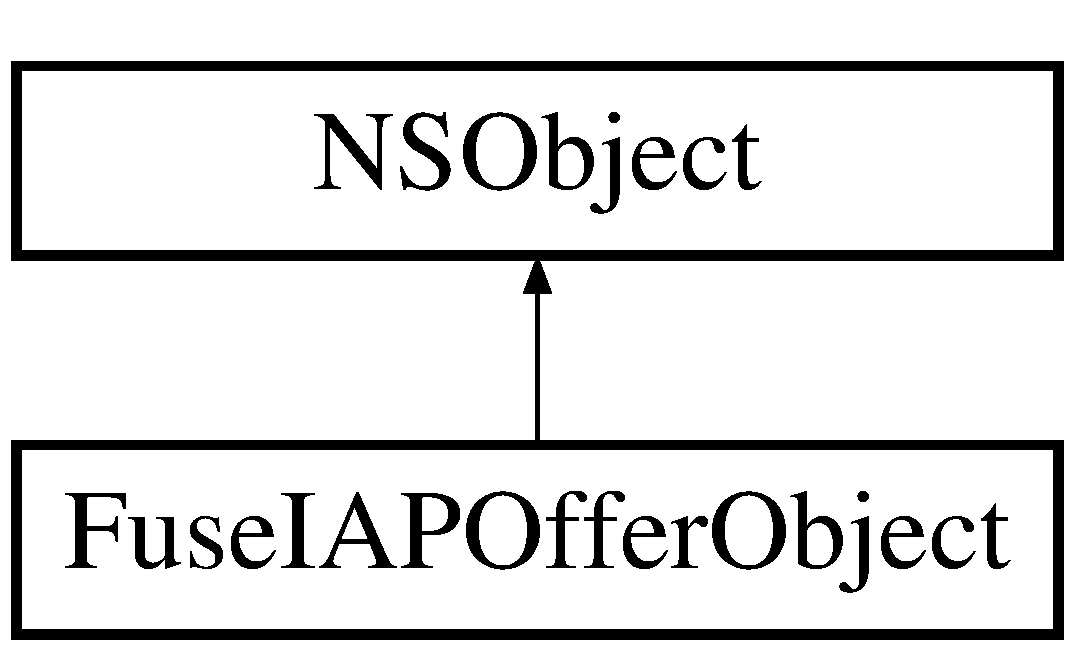
\includegraphics[height=2.000000cm]{interface_fuse_i_a_p_offer_object}
\end{center}
\end{figure}
\subsection*{Properties}
\begin{DoxyCompactItemize}
\item 
\hypertarget{interface_fuse_i_a_p_offer_object_a571e791fe7952e6d533affcd141cf8d3}{}N\+S\+String $\ast$ \hyperlink{interface_fuse_i_a_p_offer_object_a571e791fe7952e6d533affcd141cf8d3}{product\+I\+D}\label{interface_fuse_i_a_p_offer_object_a571e791fe7952e6d533affcd141cf8d3}

\begin{DoxyCompactList}\small\item\em App store product id used to complete a purchase ex. com.\+fusepowered.\+coinpack1 Set on the Dashboard. \end{DoxyCompactList}\item 
\hypertarget{interface_fuse_i_a_p_offer_object_a8d1ea52ddcdc454acacd66c011a43341}{}N\+S\+Number $\ast$ \hyperlink{interface_fuse_i_a_p_offer_object_a8d1ea52ddcdc454acacd66c011a43341}{product\+Price}\label{interface_fuse_i_a_p_offer_object_a8d1ea52ddcdc454acacd66c011a43341}

\begin{DoxyCompactList}\small\item\em Value or in local currency if available eg. 2.\+99, Default 0. \end{DoxyCompactList}\item 
\hypertarget{interface_fuse_i_a_p_offer_object_afc44eae0ea1010ef7b02515dfc156e68}{}N\+S\+String $\ast$ \hyperlink{interface_fuse_i_a_p_offer_object_afc44eae0ea1010ef7b02515dfc156e68}{item\+Name}\label{interface_fuse_i_a_p_offer_object_afc44eae0ea1010ef7b02515dfc156e68}

\begin{DoxyCompactList}\small\item\em Item name or I\+D to be given on a successful purchase. Set on the Dashboard. \end{DoxyCompactList}\item 
\hypertarget{interface_fuse_i_a_p_offer_object_a3eb537b8ee870de5085c035c1de25a31}{}N\+S\+Number $\ast$ \hyperlink{interface_fuse_i_a_p_offer_object_a3eb537b8ee870de5085c035c1de25a31}{item\+Amount}\label{interface_fuse_i_a_p_offer_object_a3eb537b8ee870de5085c035c1de25a31}

\begin{DoxyCompactList}\small\item\em Quantity of items to be purchased on successful purchase. Set on the Dashboard. \end{DoxyCompactList}\item 
\hypertarget{interface_fuse_i_a_p_offer_object_afc36b7d289310bebbe7a9979348c1a0b}{}N\+S\+String $\ast$ \hyperlink{interface_fuse_i_a_p_offer_object_afc36b7d289310bebbe7a9979348c1a0b}{metadata}\label{interface_fuse_i_a_p_offer_object_afc36b7d289310bebbe7a9979348c1a0b}

\begin{DoxyCompactList}\small\item\em Metadata passed as part of the offer. Set on the dashboard. \end{DoxyCompactList}\item 
\hypertarget{interface_fuse_i_a_p_offer_object_a498e28eb1d66c5f180a7c5b1821fa7de}{}N\+S\+Number $\ast$ \hyperlink{interface_fuse_i_a_p_offer_object_a498e28eb1d66c5f180a7c5b1821fa7de}{start\+Time}\label{interface_fuse_i_a_p_offer_object_a498e28eb1d66c5f180a7c5b1821fa7de}

\begin{DoxyCompactList}\small\item\em Start date of the offer as a unix epoch, G\+M\+T. \end{DoxyCompactList}\item 
\hypertarget{interface_fuse_i_a_p_offer_object_a25d920dd9d75005ff4a80ea4cf1b8d53}{}N\+S\+Number $\ast$ \hyperlink{interface_fuse_i_a_p_offer_object_a25d920dd9d75005ff4a80ea4cf1b8d53}{end\+Time}\label{interface_fuse_i_a_p_offer_object_a25d920dd9d75005ff4a80ea4cf1b8d53}

\begin{DoxyCompactList}\small\item\em End date of the offer as a unix epoch, G\+M\+T. \end{DoxyCompactList}\end{DoxyCompactItemize}


\subsection{Detailed Description}
Object Returned to the S\+D\+K when a I\+A\+P offer was Accepted,. 

The documentation for this class was generated from the following file\+:\begin{DoxyCompactItemize}
\item 
/\+Users/buildmachine/buildmonkey/\+Fuse\+S\+D\+Ki\+O\+S-\/master/\+Code/\+Classes/\+Fuse\+S\+D\+K/Fuse\+S\+D\+K\+Definitions.\+h\end{DoxyCompactItemize}

\hypertarget{interface_fuse_rewarded_object}{}\section{Fuse\+Rewarded\+Object Class Reference}
\label{interface_fuse_rewarded_object}\index{Fuse\+Rewarded\+Object@{Fuse\+Rewarded\+Object}}
Inheritance diagram for Fuse\+Rewarded\+Object\+:\begin{figure}[H]
\begin{center}
\leavevmode
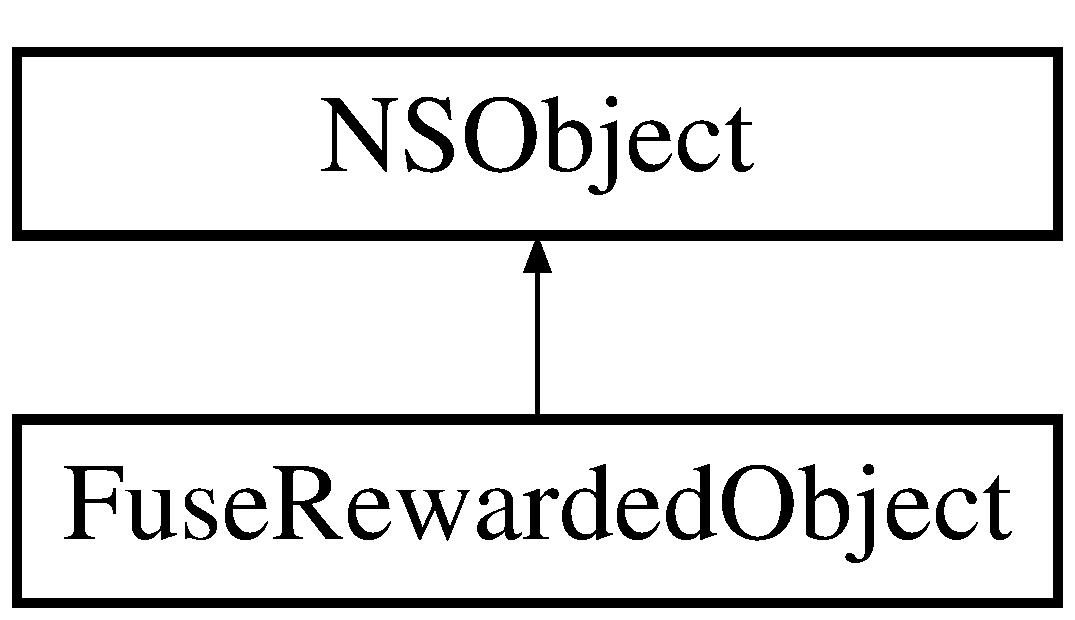
\includegraphics[height=2.000000cm]{interface_fuse_rewarded_object}
\end{center}
\end{figure}
\subsection*{Properties}
\begin{DoxyCompactItemize}
\item 
\hypertarget{interface_fuse_rewarded_object_ae1d1c7f4c017e468a6b3c1de53e5baf7}{}N\+S\+String $\ast$ {\bfseries pre\+Roll\+Message}\label{interface_fuse_rewarded_object_ae1d1c7f4c017e468a6b3c1de53e5baf7}

\item 
\hypertarget{interface_fuse_rewarded_object_acd69c101bf237f44d69b5cc310616767}{}N\+S\+String $\ast$ {\bfseries reward\+Message}\label{interface_fuse_rewarded_object_acd69c101bf237f44d69b5cc310616767}

\item 
\hypertarget{interface_fuse_rewarded_object_ac61bc6108654e4d118a6f97b79221111}{}N\+S\+String $\ast$ {\bfseries reward\+Item}\label{interface_fuse_rewarded_object_ac61bc6108654e4d118a6f97b79221111}

\item 
\hypertarget{interface_fuse_rewarded_object_a2db1b3a56b00af0fc99861443d591913}{}N\+S\+Number $\ast$ {\bfseries reward\+Amount}\label{interface_fuse_rewarded_object_a2db1b3a56b00af0fc99861443d591913}

\item 
\hypertarget{interface_fuse_rewarded_object_a07f5ea9173ecc7bdcef8797e803133d7}{}int {\bfseries item\+I\+D}\label{interface_fuse_rewarded_object_a07f5ea9173ecc7bdcef8797e803133d7}

\end{DoxyCompactItemize}


The documentation for this class was generated from the following file\+:\begin{DoxyCompactItemize}
\item 
/\+Users/buildmachine/buildmonkey/\+Fuse\+S\+D\+Ki\+O\+S-\/master/\+Code/\+Classes/\+Fuse\+S\+D\+K/Fuse\+S\+D\+K\+Definitions.\+h\end{DoxyCompactItemize}

\hypertarget{interface_fuse_s_d_k}{}\section{Fuse\+S\+D\+K Class Reference}
\label{interface_fuse_s_d_k}\index{Fuse\+S\+D\+K@{Fuse\+S\+D\+K}}


This is the main Fuse S\+D\+K static class.  




{\ttfamily \#import $<$Fuse\+S\+D\+K.\+h$>$}

Inheritance diagram for Fuse\+S\+D\+K\+:\begin{figure}[H]
\begin{center}
\leavevmode
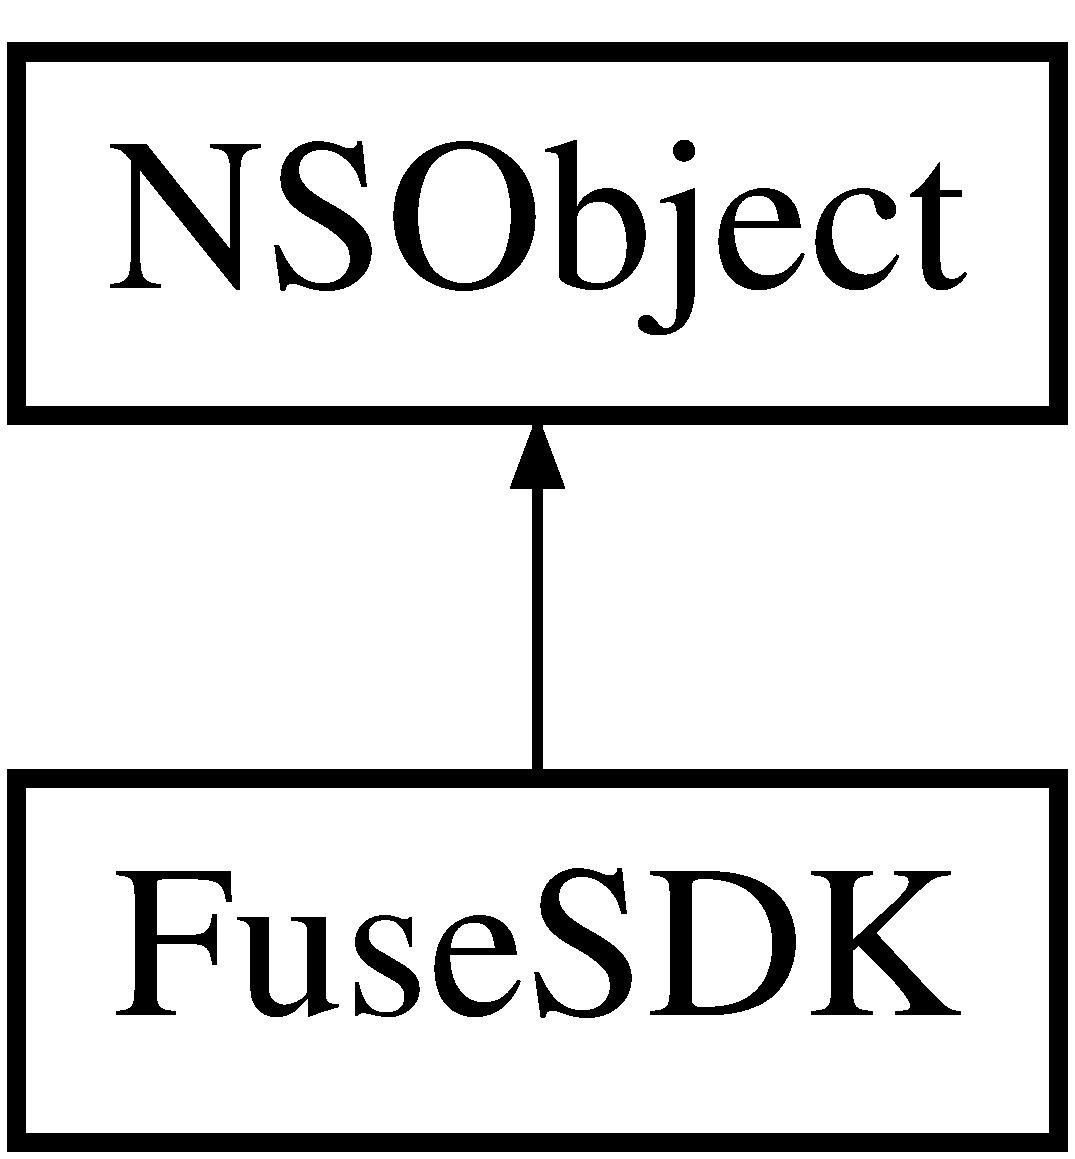
\includegraphics[height=2.000000cm]{interface_fuse_s_d_k}
\end{center}
\end{figure}
\subsection*{Instance Methods}
\begin{DoxyCompactItemize}
\item 
(N\+S\+Array $\ast$) -\/ \hyperlink{interface_fuse_s_d_k_aa268a44dea0b4db37d2d4ffa2c0ed23d}{Get\+Ad\+Zone\+List}
\begin{DoxyCompactList}\small\item\em Get a List of All active ad zones. \end{DoxyCompactList}\end{DoxyCompactItemize}
\subsection*{Class Methods}
\begin{DoxyCompactItemize}
\item 
(void) + \hyperlink{interface_fuse_s_d_k_adf7ed64a02b9540c9ded4b931ea4e400}{start\+Session\+:delegate\+:with\+Options\+:}
\begin{DoxyCompactList}\small\item\em This method is used to initiate all communication with the Fuse system (and register a $<$\hyperlink{protocol_fuse_delegate-p}{Fuse\+Delegate}$>$) \end{DoxyCompactList}\item 
(void) + \hyperlink{interface_fuse_s_d_k_a4400b7bb4b8e108c38405c47eba69b5c}{set\+Platform\+:}
\begin{DoxyCompactList}\small\item\em This method is used to describe the platform the A\+P\+I is running on. \end{DoxyCompactList}\item 
(void) + \hyperlink{interface_fuse_s_d_k_aebd93d2d4e8a6d3029134a3656b003d5}{remove\+Delegate}
\begin{DoxyCompactList}\small\item\em Removes the callback Delegate the S\+D\+K current has a reference too. \end{DoxyCompactList}\item 
(void) + \hyperlink{interface_fuse_s_d_k_a46ad48419c53d45f417d9b0561061455}{set\+Delegate\+:}
\begin{DoxyCompactList}\small\item\em Set the \hyperlink{interface_fuse_s_d_k}{Fuse\+S\+D\+K} callback Delegate. \end{DoxyCompactList}\item 
(void) + \hyperlink{interface_fuse_s_d_k_aea1b9766935aafaeb49889dc6f7cca93}{register\+For\+Push\+Token}
\begin{DoxyCompactList}\small\item\em This method is used to manually register for a push notification device token. \end{DoxyCompactList}\item 
(void) + \hyperlink{interface_fuse_s_d_k_a774f0872e0eb00528391cdc376876446}{register\+For\+Push\+Token\+:}
\begin{DoxyCompactList}\small\item\em This method is used to manually register for a push notification device token. \end{DoxyCompactList}\item 
(void) + \hyperlink{interface_fuse_s_d_k_a94479850c3b0c60887b96bb9cfa714e6}{applicationdid\+Register\+For\+Remote\+Notifications\+With\+Device\+Token\+:}
\begin{DoxyCompactList}\small\item\em This method is used to pass the registered Apple push token to the Fuse servers for future push notification messaging. \end{DoxyCompactList}\item 
(void) + \hyperlink{interface_fuse_s_d_k_ac3d0b5c1336b7a2883a6693fd4696ea0}{applicationdid\+Fail\+To\+Register\+For\+Remote\+Notifications\+With\+Error\+:}
\begin{DoxyCompactList}\small\item\em This method is used to capture when the registration of a device token has failed. \end{DoxyCompactList}\item 
(void) + \hyperlink{interface_fuse_s_d_k_a527313014384e35bf0537595295e1224}{applicationdid\+Receive\+Remote\+Notification\+:\+Application\+:}
\begin{DoxyCompactList}\small\item\em This method is used to capture when a user either receives an Apple push notification when the application is running or chooses to re-\/enter the application because of a click on an on-\/of-\/application notification . \end{DoxyCompactList}\item 
(void) + \hyperlink{interface_fuse_s_d_k_aa37c46cc4e49f09fd9b2b40a548b61fc}{respond\+To\+Application\+Launch\+Options\+:\+Application\+:}
\begin{DoxyCompactList}\small\item\em This method is optional and can collect launch options. \end{DoxyCompactList}\item 
(int) + \hyperlink{interface_fuse_s_d_k_a6956b2da78e9c5cda4006c93ddfa6718}{register\+Event\+:with\+Dict\+:}
\begin{DoxyCompactList}\small\item\em This method is used to register an named event in the Fuse system. \end{DoxyCompactList}\item 
(int) + \hyperlink{interface_fuse_s_d_k_ab95f385678dcb21bd5dbccf2ec26a760}{register\+Event\+:\+Parameter\+Name\+:\+Parameter\+Value\+:\+Variables\+:}
\begin{DoxyCompactList}\small\item\em This method will send a named event (with values) to the Fuse system for tracking. \end{DoxyCompactList}\item 
(int) + \hyperlink{interface_fuse_s_d_k_a1d6a85a81319fc97ee45e597a086fe0d}{register\+Event\+:\+Parameter\+Name\+:\+Parameter\+Value\+:\+Variable\+Name\+:\+Variable\+Value\+:}
\begin{DoxyCompactList}\small\item\em This method will send a named event (with values) to the Fuse system for tracking. \end{DoxyCompactList}\item 
(void) + \hyperlink{interface_fuse_s_d_k_a9afd8c386a2b6664641da19fa64072c9}{register\+Crash\+:}
\begin{DoxyCompactList}\small\item\em This method is used to catch crashes within an app. \end{DoxyCompactList}\item 
(void) + \hyperlink{interface_fuse_s_d_k_ab1029e5beb592f22c1ba0deea9e7bd1c}{register\+In\+App\+Purchase\+List\+:}
\begin{DoxyCompactList}\small\item\em This method is used to register the price and currency that a user is using to make an in-\/app purchase. \end{DoxyCompactList}\item 
(void) + \hyperlink{interface_fuse_s_d_k_a2dd50722daab117889c396ff58fe7c27}{register\+In\+App\+Purchase\+:}
\begin{DoxyCompactList}\small\item\em This method records in-\/app purchases in the Fuse system. \end{DoxyCompactList}\item 
(void) + \hyperlink{interface_fuse_s_d_k_a8a1846c84fa16e45488e797dca4c7aaa}{register\+In\+App\+Purchase\+:\+Tx\+State\+:\+Price\+:\+Currency\+:\+Product\+I\+D\+:}
\begin{DoxyCompactList}\small\item\em This method records in-\/app purchases in the Fuse system without using the S\+K\+Payment\+Transaction data type. \end{DoxyCompactList}\item 
(void) + \hyperlink{interface_fuse_s_d_k_a2115a4fac03204fd73699ab9ea3314f5}{register\+In\+App\+Purchase\+:\+Tx\+State\+:\+Price\+:\+Currency\+:\+Product\+I\+D\+:\+Transaction\+I\+D\+:}
\begin{DoxyCompactList}\small\item\em This method records in-\/app purchases in the Fuse system without using the S\+K\+Payment\+Transaction data type. \end{DoxyCompactList}\item 
(B\+O\+O\+L) + \hyperlink{interface_fuse_s_d_k_abdf624c4ef56ee1c7cac73b37dc4f5fd}{is\+Ad\+Available\+For\+Zone\+I\+D\+:}
\begin{DoxyCompactList}\small\item\em This method returns if an ad was loaded in a particular zone. \end{DoxyCompactList}\item 
(void) + \hyperlink{interface_fuse_s_d_k_aba0c488866771c47887ac847c2cd884e}{show\+Ad\+For\+Zone\+I\+D\+:options\+:}
\begin{DoxyCompactList}\small\item\em This method displays a Fuse interstitial ad for a given ad zone. Different ad zones can be configured via the Fuse Dashboard. \end{DoxyCompactList}\item 
(void) + \hyperlink{interface_fuse_s_d_k_a2e80d673366877a4bcfc6fe86031d526}{preload\+Ad\+For\+Zone\+I\+D\+:}
\begin{DoxyCompactList}\small\item\em This method loads an ad and reports if it is available to be shown to the user for the specified ad zone. \end{DoxyCompactList}\item 
(\hyperlink{interface_fuse_rewarded_object}{Fuse\+Rewarded\+Object} $\ast$) + \hyperlink{interface_fuse_s_d_k_a89958c6b87beffac157ac028e9e29df1}{get\+Rewarded\+Info\+For\+Zone\+I\+D\+:}
\begin{DoxyCompactList}\small\item\em This Method returns the \hyperlink{interface_fuse_rewarded_object}{Fuse\+Rewarded\+Object} for a give zone\+I\+D, or nil if there is no rewards available. \end{DoxyCompactList}\item 
(B\+O\+O\+L) + \hyperlink{interface_fuse_s_d_k_ad98a95cc63498dee7256258206808056}{zone\+Has\+Rewarded\+:}
\begin{DoxyCompactList}\small\item\em Use this method to query wether or not an ad zone has rewarded video content in it;. \end{DoxyCompactList}\item 
(B\+O\+O\+L) + \hyperlink{interface_fuse_s_d_k_adb67f99bc2972de6774949fc2849f548}{zone\+Has\+I\+A\+P\+Offer\+:}
\begin{DoxyCompactList}\small\item\em Use this method to query wether or not an ad zone has iap offer content in it;. \end{DoxyCompactList}\item 
(B\+O\+O\+L) + \hyperlink{interface_fuse_s_d_k_a898ce4e1d5235fd40627429d1f7bf138}{zone\+Has\+Virtual\+Goods\+Offer\+:}
\begin{DoxyCompactList}\small\item\em Use this method to query wether or not an ad zone has virtual goods content;. \end{DoxyCompactList}\item 
(void) + \hyperlink{interface_fuse_s_d_k_a279e4cb8e95a3e78197761156a7de50d}{display\+Notifications}
\begin{DoxyCompactList}\small\item\em This method is used to display in-\/game Fuse notifications. \end{DoxyCompactList}\item 
\hypertarget{interface_fuse_s_d_k_a23c30bc15f208daf639ece250b8a5935}{}(B\+O\+O\+L) + \hyperlink{interface_fuse_s_d_k_a23c30bc15f208daf639ece250b8a5935}{is\+Notification\+Available}\label{interface_fuse_s_d_k_a23c30bc15f208daf639ece250b8a5935}

\begin{DoxyCompactList}\small\item\em This method returns whether a Fuse notification is available to be viewed. \end{DoxyCompactList}\item 
(void) + \hyperlink{interface_fuse_s_d_k_ac7c361dc8e2935cbd32cbdd6c5c8952b}{display\+More\+Games}
\begin{DoxyCompactList}\small\item\em This method is use to display the \char`\"{}\+More Games\char`\"{} section. \end{DoxyCompactList}\item 
(void) + \hyperlink{interface_fuse_s_d_k_a2b0c7be7abc4ec4ae6912f295d21e64c}{register\+Gender\+:}
\begin{DoxyCompactList}\small\item\em This method registers a gender for the user. \end{DoxyCompactList}\item 
(void) + \hyperlink{interface_fuse_s_d_k_a33903ca8d52be440186c4bbf1cbe510c}{register\+Age\+:}
\begin{DoxyCompactList}\small\item\em This method registers an age for the user. \end{DoxyCompactList}\item 
(void) + \hyperlink{interface_fuse_s_d_k_a5dcbaec8b00d90c4970e1b752e5dc719}{register\+Birthday\+:\+Month\+:\+Day\+:}
\begin{DoxyCompactList}\small\item\em This method registers a user's birthday. \end{DoxyCompactList}\item 
(N\+S\+String $\ast$) + \hyperlink{interface_fuse_s_d_k_ab483c2a3f4439aad8e19200cf24ff731}{get\+Fuse\+I\+D}
\begin{DoxyCompactList}\small\item\em This method returns the public 'Fuse I\+D'. \end{DoxyCompactList}\item 
(void) + \hyperlink{interface_fuse_s_d_k_a02a3bc5562d4f6e50bac5339f4ac4046}{game\+Center\+Login\+:}
\begin{DoxyCompactList}\small\item\em Game Center account registration. \end{DoxyCompactList}\item 
(void) + \hyperlink{interface_fuse_s_d_k_a7003a2102cba9c87fa127e39c95a5d1d}{facebook\+Login\+:\+Name\+:with\+Access\+Token\+:}
\begin{DoxyCompactList}\small\item\em Facebook account registration. \end{DoxyCompactList}\item 
(void) + \hyperlink{interface_fuse_s_d_k_a04c181e3ec49e81ba081a5041df412f6}{facebook\+Login\+:}
\begin{DoxyCompactList}\small\item\em Facebook account registration. \end{DoxyCompactList}\item 
(void) + \hyperlink{interface_fuse_s_d_k_a38487be821059910b1b939d818cd0e9f}{facebook\+Login\+:\+Name\+:\+Gender\+:with\+Access\+Token\+:}
\begin{DoxyCompactList}\small\item\em Facebook account registration. \end{DoxyCompactList}\item 
(void) + \hyperlink{interface_fuse_s_d_k_add5138c113d6e4c1201f70bf8b84eb02}{twitter\+Login\+:}
\begin{DoxyCompactList}\small\item\em Twitter account registration. \end{DoxyCompactList}\item 
(void) + \hyperlink{interface_fuse_s_d_k_a48950b5880ce336cc601a752bcda1a3a}{twitter\+Login\+:\+Alias\+:}
\begin{DoxyCompactList}\small\item\em Twitter account registration with user name. \end{DoxyCompactList}\item 
(void) + \hyperlink{interface_fuse_s_d_k_af7b69ec93b7a26b8512d730db9383511}{fuse\+Login\+:\+Alias\+:}
\begin{DoxyCompactList}\small\item\em Fuse account registration. \end{DoxyCompactList}\item 
(void) + \hyperlink{interface_fuse_s_d_k_a6b16a24e8cb2fdd04b8be9e501259135}{email\+Login\+:\+Alias\+:}
\begin{DoxyCompactList}\small\item\em Account registration using an email address. \end{DoxyCompactList}\item 
(void) + \hyperlink{interface_fuse_s_d_k_ae3a27f858739fee7ad6483a909206943}{device\+Login\+:}
\begin{DoxyCompactList}\small\item\em Account registration using the unique device identifier. \end{DoxyCompactList}\item 
(void) + \hyperlink{interface_fuse_s_d_k_a826545aa45a550cbc10cc98137ee5898}{google\+Play\+Login\+:\+Access\+Token\+:}
\begin{DoxyCompactList}\small\item\em Account registration using the google play login identifier. \end{DoxyCompactList}\item 
(N\+S\+String $\ast$) + \hyperlink{interface_fuse_s_d_k_a49b43f13a0efee7d2af60197d0ae341c}{get\+Original\+Account\+I\+D}
\begin{DoxyCompactList}\small\item\em Get the original account I\+D used to log in to the Fuse system that corresponds to the Fuse I\+D. \end{DoxyCompactList}\item 
(int) + \hyperlink{interface_fuse_s_d_k_a0571f2d960109dc9bff59c6575bf2534}{get\+Original\+Account\+Type}
\begin{DoxyCompactList}\small\item\em Get the original account type used to log in to the Fuse system that corresponds to the Fuse I\+D. \end{DoxyCompactList}\item 
(N\+S\+String $\ast$) + \hyperlink{interface_fuse_s_d_k_ab49bb189bd1ebaf871f24a7c4e4b5290}{get\+Original\+Account\+Alias}
\begin{DoxyCompactList}\small\item\em Get the original account alias of the user used to log in to the Fuse system. \end{DoxyCompactList}\item 
(int) + \hyperlink{interface_fuse_s_d_k_afb8604dccdbf7c0b507074a649b75da9}{games\+Played}
\begin{DoxyCompactList}\small\item\em This method returns the amount of times the user has opened the application. \end{DoxyCompactList}\item 
(N\+S\+String $\ast$) + \hyperlink{interface_fuse_s_d_k_a56f5fc3ba2e03d3dbe9d681b3500108a}{library\+Version}
\begin{DoxyCompactList}\small\item\em This method returns the Fuse S\+D\+K version. \end{DoxyCompactList}\item 
(B\+O\+O\+L) + \hyperlink{interface_fuse_s_d_k_a6db77bb2cb4ba38f58666edfa470f7bd}{connected}
\begin{DoxyCompactList}\small\item\em This method indicates whether the application is connected to the internet. \end{DoxyCompactList}\item 
(void) + \hyperlink{interface_fuse_s_d_k_a60de732b9ecb7bce2439517cc2ca1f71}{utc\+Time\+From\+Server}
\begin{DoxyCompactList}\small\item\em This method gets the U\+T\+C time from the server. \end{DoxyCompactList}\item 
(B\+O\+O\+L) + \hyperlink{interface_fuse_s_d_k_adb24897bb2dd5a7521d1f7c3cb6e0d4d}{not\+Ready\+To\+Terminate}
\begin{DoxyCompactList}\small\item\em This method indicates whether the Fuse S\+D\+K has concluded all necessary work before being able to be closed. \end{DoxyCompactList}\item 
(void) + \hyperlink{interface_fuse_s_d_k_a70b5812f76a70821e3d6de1ac9e44c04}{disable\+Data}
\begin{DoxyCompactList}\small\item\em This method opts a user out of data being collected by the A\+P\+I. \end{DoxyCompactList}\item 
(void) + \hyperlink{interface_fuse_s_d_k_a8c0d55b6f8fad28e9cb150271a82df2f}{enable\+Data}
\begin{DoxyCompactList}\small\item\em This method opts a user in so that data is collected by the A\+P\+I. \end{DoxyCompactList}\item 
(B\+O\+O\+L) + \hyperlink{interface_fuse_s_d_k_a0462d911d4b1aec0c9e4ff77f3acd6fa}{data\+Enabled}
\begin{DoxyCompactList}\small\item\em This method indicates whether the user is opted-\/in to collecting data. \end{DoxyCompactList}\item 
(void) + \hyperlink{interface_fuse_s_d_k_a11a92658dca5be9d79ca19a66bafb91e}{update\+Friends\+List\+From\+Server}
\begin{DoxyCompactList}\small\item\em Get a the user's friends list. \end{DoxyCompactList}\item 
(N\+S\+Mutable\+Dictionary $\ast$) + \hyperlink{interface_fuse_s_d_k_a31d609ce39be3e6eda04fd32d8036e95}{get\+Friends\+List}
\begin{DoxyCompactList}\small\item\em This method returns the local friends list of the logged in user. \end{DoxyCompactList}\item 
(void) + \hyperlink{interface_fuse_s_d_k_a92b5888d1e5dafe2ab2a76fda44be4d8}{add\+Friend\+:}
\begin{DoxyCompactList}\small\item\em This method is used to invite (add) a friend to the logged in user's friends list. \end{DoxyCompactList}\item 
(void) + \hyperlink{interface_fuse_s_d_k_a1556fd18ab2ae7f062c9d2ebbe2498fc}{remove\+Friend\+:}
\begin{DoxyCompactList}\small\item\em This method is used to delete a friend from the logged in user's friends list. \end{DoxyCompactList}\item 
(void) + \hyperlink{interface_fuse_s_d_k_ae93cfa17f5b00ab1d28c53a8577c1af0}{accept\+Friend\+:}
\begin{DoxyCompactList}\small\item\em This method is used to accept a friend request. \end{DoxyCompactList}\item 
(void) + \hyperlink{interface_fuse_s_d_k_a8af1416799fd2922db49ed1de406f537}{reject\+Friend\+:}
\begin{DoxyCompactList}\small\item\em This method is used to reject a friend request. \end{DoxyCompactList}\item 
(void) + \hyperlink{interface_fuse_s_d_k_a199e36abe741ecdf8062d1afddc6e146}{migrate\+Friends\+:}
\begin{DoxyCompactList}\small\item\em This method is used to migrate (one-\/way) friends from an existing account to the logged in user's friends list. \end{DoxyCompactList}\item 
(void) + \hyperlink{interface_fuse_s_d_k_a84916a862fe925004f0c2d3c2b16aa28}{user\+Push\+Notification\+:\+Message\+:}
\begin{DoxyCompactList}\small\item\em Send an Apple push notification to another user. \end{DoxyCompactList}\item 
(void) + \hyperlink{interface_fuse_s_d_k_a9afa8ec3f16cd18706902dd1f38c3501}{friends\+Push\+Notification\+:}
\begin{DoxyCompactList}\small\item\em Send an Apple push notification to a user's entire friends list. \end{DoxyCompactList}\item 
(void) + \hyperlink{interface_fuse_s_d_k_a37448397d10db8278e2e45d0448c4fa0}{register\+Level\+:}
\begin{DoxyCompactList}\small\item\em Register the user's current level after they level-\/up. \end{DoxyCompactList}\item 
(void) + \hyperlink{interface_fuse_s_d_k_ac07a77edd3b1eeddfe96dba096f15273}{register\+Currency\+:\+Balance\+:}
\begin{DoxyCompactList}\small\item\em Register a change in the current balances of the user's in-\/app currencies. \end{DoxyCompactList}\item 
(N\+S\+String $\ast$) + \hyperlink{interface_fuse_s_d_k_ab29213306801eba35d922754a5efa1b0}{get\+Game\+Configuration\+Value\+:}
\begin{DoxyCompactList}\small\item\em This method retrieves server configuration values. \end{DoxyCompactList}\item 
(N\+S\+Mutable\+Dictionary $\ast$) + \hyperlink{interface_fuse_s_d_k_a0267e0bb12395c93cea9442f62dcc53e}{get\+Game\+Configuration}
\begin{DoxyCompactList}\small\item\em This method retrieves the entire server configuration value list. \end{DoxyCompactList}\item 
(instancetype) + \hyperlink{interface_fuse_s_d_k_a01b0d405cef0701ca335624d9910fa6f}{get}
\begin{DoxyCompactList}\small\item\em Singleton accessor for the \hyperlink{interface_fuse_s_d_k}{Fuse\+S\+D\+K} class. \end{DoxyCompactList}\end{DoxyCompactItemize}
\subsection*{Protected Attributes}
\begin{DoxyCompactItemize}
\item 
\hypertarget{interface_fuse_s_d_k_a9f31440253247f4852ff50a170c05231}{}N\+S\+Object$<$ \hyperlink{protocol_fuse_delegate-p}{Fuse\+Delegate} $>$ $\ast$ {\bfseries delegate}\label{interface_fuse_s_d_k_a9f31440253247f4852ff50a170c05231}

\end{DoxyCompactItemize}


\subsection{Detailed Description}
This is the main Fuse S\+D\+K static class. 

\subsection{Method Documentation}
\hypertarget{interface_fuse_s_d_k_ae93cfa17f5b00ab1d28c53a8577c1af0}{}\index{Fuse\+S\+D\+K@{Fuse\+S\+D\+K}!accept\+Friend\+:@{accept\+Friend\+:}}
\index{accept\+Friend\+:@{accept\+Friend\+:}!Fuse\+S\+D\+K@{Fuse\+S\+D\+K}}
\subsubsection[{accept\+Friend\+:}]{\setlength{\rightskip}{0pt plus 5cm}+ (void) accept\+Friend\+: 
\begin{DoxyParamCaption}
\item[{(N\+S\+String $\ast$)}]{\+\_\+fuse\+\_\+id}
\end{DoxyParamCaption}
}\label{interface_fuse_s_d_k_ae93cfa17f5b00ab1d28c53a8577c1af0}


This method is used to accept a friend request. 

The inviting of a friend is a two-\/step process. The first step is to actually invite the user (source user) using add\+Friend\+:, and the second step is the acceptance by the target user using this method. If a $<$\hyperlink{protocol_fuse_delegate-p}{Fuse\+Delegate}$>$ has been registered using start\+Session\+:delegate\+:with\+Options\+:, a callback can be made once the friend is accepted (in case a notification is required by the application).

To accept a user\+:


\begin{DoxyCode}
[\hyperlink{interface_fuse_s_d_k}{FuseSDK} acceptFriend:\textcolor{stringliteral}{@"012345678"}];
\end{DoxyCode}


The (optional) callback to the $<$\hyperlink{protocol_fuse_delegate-p}{Fuse\+Delegate}$>$ is as follows\+:


\begin{DoxyCode}
-(void) friendAccepted:(NSString*)\_fuse\_id Error:(NSError*)\_error
\{
   \textcolor{comment}{// A friend has been marked as accepted on the server}
   \textcolor{comment}{// If [error intValue] != 0, an error has occurred}
   \textcolor{comment}{// Please see EFuseError for more information on all of the possible error codes}
\}
\end{DoxyCode}



\begin{DoxyParams}{Parameters}
{\em \+\_\+fuse\+\_\+id} & \mbox{[}N\+S\+String$\ast$\mbox{]} This is the \char`\"{}\+Fuse I\+D\char`\"{} of the player being accepted \\
\hline
\end{DoxyParams}
\begin{DoxySeeAlso}{See also}
\hyperlink{interface_fuse_s_d_k_adf7ed64a02b9540c9ded4b931ea4e400}{+ start\+Session\+:delegate\+:with\+Options\+:} for information on setting up the $<$\hyperlink{protocol_fuse_delegate-p}{Fuse\+Delegate}$>$ 

\hyperlink{interface_fuse_s_d_k_a92b5888d1e5dafe2ab2a76fda44be4d8}{+ add\+Friend\+:} for more information on adding a friend and the handshaking process 

\hyperlink{protocol_fuse_delegate-p_ab48f8ef85f4f32654af102c5fa09c4c1}{-\/ friend\+Accepted\+:\+Error\+: (\+Fuse\+Delegate-\/p)} for more information on the delegate method 
\end{DoxySeeAlso}
\begin{DoxySince}{Since}
Fuse S\+D\+K version 1.\+22 
\end{DoxySince}
\hypertarget{interface_fuse_s_d_k_a92b5888d1e5dafe2ab2a76fda44be4d8}{}\index{Fuse\+S\+D\+K@{Fuse\+S\+D\+K}!add\+Friend\+:@{add\+Friend\+:}}
\index{add\+Friend\+:@{add\+Friend\+:}!Fuse\+S\+D\+K@{Fuse\+S\+D\+K}}
\subsubsection[{add\+Friend\+:}]{\setlength{\rightskip}{0pt plus 5cm}+ (void) add\+Friend\+: 
\begin{DoxyParamCaption}
\item[{(N\+S\+String $\ast$)}]{\+\_\+fuse\+\_\+id}
\end{DoxyParamCaption}
}\label{interface_fuse_s_d_k_a92b5888d1e5dafe2ab2a76fda44be4d8}


This method is used to invite (add) a friend to the logged in user's friends list. 

A friend is not added right away to the inviting user's list. Instead, there is a handshaking mechanism whereby the invited user needs to agree to the invite (see accept\+Friend\+:) before both users are shown in each others list. If a $<$\hyperlink{protocol_fuse_delegate-p}{Fuse\+Delegate}$>$ has been registered using start\+Session\+:delegate\+:with\+Options\+:, a callback can be made once the friend is added (in case a notification is required by the application).

To add a friend\+:


\begin{DoxyCode}
[\hyperlink{interface_fuse_s_d_k}{FuseSDK} addFriend:\textcolor{stringliteral}{@"012345678"}];
\end{DoxyCode}


The (optional) callback to the $<$\hyperlink{protocol_fuse_delegate-p}{Fuse\+Delegate}$>$ is as follows\+:


\begin{DoxyCode}
-(void) friendAdded:(NSString*)\_fuse\_id Error:(NSError*)\_error
\{
   \textcolor{comment}{// A friend has been added}
   \textcolor{comment}{// If [error intValue] != 0, an error has occurred}
   \textcolor{comment}{// Please see EFuseError for more information on all of the possible error codes}
\}
\end{DoxyCode}



\begin{DoxyParams}{Parameters}
{\em \+\_\+fuse\+\_\+id} & \mbox{[}N\+S\+String$\ast$\mbox{]} This is the \char`\"{}\+Fuse I\+D\char`\"{} of the player being invited \\
\hline
\end{DoxyParams}
\begin{DoxySeeAlso}{See also}
\hyperlink{interface_fuse_s_d_k_adf7ed64a02b9540c9ded4b931ea4e400}{+ start\+Session\+:delegate\+:with\+Options\+:} for information on setting up the $<$\hyperlink{protocol_fuse_delegate-p}{Fuse\+Delegate}$>$ 

\hyperlink{protocol_fuse_delegate-p_a5c1b86ecfdc9518f976d5ea96156b408}{-\/ friend\+Added\+:\+Error\+: (\+Fuse\+Delegate-\/p)} for more information on the delegate method 
\end{DoxySeeAlso}
\begin{DoxySince}{Since}
Fuse S\+D\+K version 1.\+22 
\end{DoxySince}
\hypertarget{interface_fuse_s_d_k_ac3d0b5c1336b7a2883a6693fd4696ea0}{}\index{Fuse\+S\+D\+K@{Fuse\+S\+D\+K}!applicationdid\+Fail\+To\+Register\+For\+Remote\+Notifications\+With\+Error\+:@{applicationdid\+Fail\+To\+Register\+For\+Remote\+Notifications\+With\+Error\+:}}
\index{applicationdid\+Fail\+To\+Register\+For\+Remote\+Notifications\+With\+Error\+:@{applicationdid\+Fail\+To\+Register\+For\+Remote\+Notifications\+With\+Error\+:}!Fuse\+S\+D\+K@{Fuse\+S\+D\+K}}
\subsubsection[{applicationdid\+Fail\+To\+Register\+For\+Remote\+Notifications\+With\+Error\+:}]{\setlength{\rightskip}{0pt plus 5cm}+ (void) applicationdid\+Fail\+To\+Register\+For\+Remote\+Notifications\+With\+Error\+: 
\begin{DoxyParamCaption}
\item[{(N\+S\+Error $\ast$)}]{error}
\end{DoxyParamCaption}
}\label{interface_fuse_s_d_k_ac3d0b5c1336b7a2883a6693fd4696ea0}


This method is used to capture when the registration of a device token has failed. 


\begin{DoxyParams}{Parameters}
{\em error} & \mbox{[}N\+S\+Error$\ast$\mbox{]} This method should be called from your application delegate file application\+:did\+Fail\+To\+Register\+For\+Remote\+Notifications\+With\+Error method\+:\\
\hline
\end{DoxyParams}

\begin{DoxyCode}
- (void)application:(UIApplication *)application didFailToRegisterForRemoteNotificationsWithError:(NSError 
      *)error 
\{
   [\hyperlink{interface_fuse_s_d_k}{FuseSDK} applicationdidFailToRegisterForRemoteNotificationsWithError:error];
\}
\end{DoxyCode}



\begin{DoxyParams}{Parameters}
{\em error} & \mbox{[}N\+S\+Error$\ast$\mbox{]} The error passed to application\+:did\+Fail\+To\+Register\+For\+Remote\+Notifications\+With\+Error \\
\hline
\end{DoxyParams}
\hypertarget{interface_fuse_s_d_k_a527313014384e35bf0537595295e1224}{}\index{Fuse\+S\+D\+K@{Fuse\+S\+D\+K}!applicationdid\+Receive\+Remote\+Notification\+:\+Application\+:@{applicationdid\+Receive\+Remote\+Notification\+:\+Application\+:}}
\index{applicationdid\+Receive\+Remote\+Notification\+:\+Application\+:@{applicationdid\+Receive\+Remote\+Notification\+:\+Application\+:}!Fuse\+S\+D\+K@{Fuse\+S\+D\+K}}
\subsubsection[{applicationdid\+Receive\+Remote\+Notification\+:\+Application\+:}]{\setlength{\rightskip}{0pt plus 5cm}+ (void) applicationdid\+Receive\+Remote\+Notification\+: 
\begin{DoxyParamCaption}
\item[{(N\+S\+Dictionary $\ast$)}]{user\+Info}
\item[{Application:(U\+I\+Application $\ast$)}]{application}
\end{DoxyParamCaption}
}\label{interface_fuse_s_d_k_a527313014384e35bf0537595295e1224}


This method is used to capture when a user either receives an Apple push notification when the application is running or chooses to re-\/enter the application because of a click on an on-\/of-\/application notification . 

This method is very important in determining the effectiveness of a push notification in terms of winning back users to the application. This method should be called from your application delegate file application\+:did\+Fail\+To\+Register\+For\+Remote\+Notifications\+With\+Error method\+:


\begin{DoxyCode}
- (void)application:(UIApplication *)application didReceiveRemoteNotification:(NSDictionary *)userInfo
\{
   [\hyperlink{interface_fuse_s_d_k}{FuseSDK} applicationdidReceiveRemoteNotification:userInfo Application:application];  
\}
\end{DoxyCode}



\begin{DoxyParams}{Parameters}
{\em user\+Info} & \mbox{[}N\+S\+Dictionary$\ast$\mbox{]} The information dictionary passed to application\+:did\+Receive\+Remote\+Notification \\
\hline
{\em application} & \mbox{[}U\+I\+Application$\ast$\mbox{]} The initiating U\+I\+Application instance \\
\hline
\end{DoxyParams}
\begin{DoxySeeAlso}{See also}
\hyperlink{interface_fuse_s_d_k_a94479850c3b0c60887b96bb9cfa714e6}{+ applicationdid\+Register\+For\+Remote\+Notifications\+With\+Device\+Token\+:} for more information on collecting tokens. 
\end{DoxySeeAlso}
\hypertarget{interface_fuse_s_d_k_a94479850c3b0c60887b96bb9cfa714e6}{}\index{Fuse\+S\+D\+K@{Fuse\+S\+D\+K}!applicationdid\+Register\+For\+Remote\+Notifications\+With\+Device\+Token\+:@{applicationdid\+Register\+For\+Remote\+Notifications\+With\+Device\+Token\+:}}
\index{applicationdid\+Register\+For\+Remote\+Notifications\+With\+Device\+Token\+:@{applicationdid\+Register\+For\+Remote\+Notifications\+With\+Device\+Token\+:}!Fuse\+S\+D\+K@{Fuse\+S\+D\+K}}
\subsubsection[{applicationdid\+Register\+For\+Remote\+Notifications\+With\+Device\+Token\+:}]{\setlength{\rightskip}{0pt plus 5cm}+ (void) applicationdid\+Register\+For\+Remote\+Notifications\+With\+Device\+Token\+: 
\begin{DoxyParamCaption}
\item[{(N\+S\+Data $\ast$)}]{device\+Token}
\end{DoxyParamCaption}
}\label{interface_fuse_s_d_k_a94479850c3b0c60887b96bb9cfa714e6}


This method is used to pass the registered Apple push token to the Fuse servers for future push notification messaging. 

This method should be called from your application delegate file application\+:did\+Register\+For\+Remote\+Notifications\+With\+Device\+Token method\+:


\begin{DoxyCode}
- (void)application:(UIApplication *)application didRegisterForRemoteNotificationsWithDeviceToken:(NSData 
      *)deviceToken 
\{
   [\hyperlink{interface_fuse_s_d_k}{FuseSDK} applicationdidRegisterForRemoteNotificationsWithDeviceToken:deviceToken];
\}
\end{DoxyCode}



\begin{DoxyParams}{Parameters}
{\em device\+Token} & \mbox{[}N\+S\+Data$\ast$\mbox{]} The device token passed to application\+:did\+Register\+For\+Remote\+Notifications\+With\+Device\+Token \\
\hline
\end{DoxyParams}
\hypertarget{interface_fuse_s_d_k_a6db77bb2cb4ba38f58666edfa470f7bd}{}\index{Fuse\+S\+D\+K@{Fuse\+S\+D\+K}!connected@{connected}}
\index{connected@{connected}!Fuse\+S\+D\+K@{Fuse\+S\+D\+K}}
\subsubsection[{connected}]{\setlength{\rightskip}{0pt plus 5cm}+ (B\+O\+O\+L) connected 
\begin{DoxyParamCaption}
{}
\end{DoxyParamCaption}
}\label{interface_fuse_s_d_k_a6db77bb2cb4ba38f58666edfa470f7bd}


This method indicates whether the application is connected to the internet. 

This method indicates if the application is connected via wifi or cellular network and connected to the internet. To use this method\+:


\begin{DoxyCode}
BOOL is\_connected = [\hyperlink{interface_fuse_s_d_k}{FuseSDK} \hyperlink{interface_fuse_s_d_k_a6db77bb2cb4ba38f58666edfa470f7bd}{connected}];
\end{DoxyCode}



\begin{DoxyRetVals}{Return values}
{\em \mbox{[}\+B\+O\+O\+L\mbox{]}} & The connected status of the application \\
\hline
\end{DoxyRetVals}
\hypertarget{interface_fuse_s_d_k_a0462d911d4b1aec0c9e4ff77f3acd6fa}{}\index{Fuse\+S\+D\+K@{Fuse\+S\+D\+K}!data\+Enabled@{data\+Enabled}}
\index{data\+Enabled@{data\+Enabled}!Fuse\+S\+D\+K@{Fuse\+S\+D\+K}}
\subsubsection[{data\+Enabled}]{\setlength{\rightskip}{0pt plus 5cm}+ (B\+O\+O\+L) data\+Enabled 
\begin{DoxyParamCaption}
{}
\end{DoxyParamCaption}
}\label{interface_fuse_s_d_k_a0462d911d4b1aec0c9e4ff77f3acd6fa}


This method indicates whether the user is opted-\/in to collecting data. 

To see if a user has indicated whether they want data collected\+:


\begin{DoxyCode}
BOOL is\_opted\_in = [\hyperlink{interface_fuse_s_d_k}{FuseSDK} \hyperlink{interface_fuse_s_d_k_a0462d911d4b1aec0c9e4ff77f3acd6fa}{dataEnabled}];
\end{DoxyCode}



\begin{DoxyRetVals}{Return values}
{\em \mbox{[}\+B\+O\+O\+L\mbox{]}} & Indicates if the user has enabled data to be collected \\
\hline
\end{DoxyRetVals}
\hypertarget{interface_fuse_s_d_k_ae3a27f858739fee7ad6483a909206943}{}\index{Fuse\+S\+D\+K@{Fuse\+S\+D\+K}!device\+Login\+:@{device\+Login\+:}}
\index{device\+Login\+:@{device\+Login\+:}!Fuse\+S\+D\+K@{Fuse\+S\+D\+K}}
\subsubsection[{device\+Login\+:}]{\setlength{\rightskip}{0pt plus 5cm}+ (void) device\+Login\+: 
\begin{DoxyParamCaption}
\item[{(N\+S\+String $\ast$)}]{\+\_\+alias}
\end{DoxyParamCaption}
}\label{interface_fuse_s_d_k_ae3a27f858739fee7ad6483a909206943}


Account registration using the unique device identifier. 

Uniquely track a user based upon their device identifier. This system can be used in conjunction with the 'set' and 'get' game data to persist per-\/user. However, this system cannot track users across devices since it is tied to a device. The main benefit to using this call to \char`\"{}log\char`\"{} a user in to the system is to avoid any other sign-\/in (like Facebook or Game Center).

To call this method\+:


\begin{DoxyCode}
[\hyperlink{interface_fuse_s_d_k}{FuseSDK} deviceLogin:\textcolor{stringliteral}{@"Geronimo"}];
\end{DoxyCode}


If required, a callback is sent to the $<$\hyperlink{protocol_fuse_delegate-p}{Fuse\+Delegate}$>$ (if registered) indicating that the Fuse system has received the login information.


\begin{DoxyCode}
-(void) accountLoginComplete:(NSNumber*)\_type Account:(NSString*)\_account\_id;
\end{DoxyCode}



\begin{DoxyParams}{Parameters}
{\em \+\_\+alias} & \mbox{[}N\+S\+String$\ast$\mbox{]} The alias or 'handle' of the user \\
\hline
\end{DoxyParams}
\begin{DoxySince}{Since}
Fuse S\+D\+K version 1.\+25 
\end{DoxySince}
\begin{DoxySeeAlso}{See also}
\hyperlink{interface_fuse_s_d_k_adf7ed64a02b9540c9ded4b931ea4e400}{+ start\+Session\+:delegate\+:with\+Options\+:} to see how to register a $<$\hyperlink{protocol_fuse_delegate-p}{Fuse\+Delegate}$>$ object to receive the optional callback 

\hyperlink{protocol_fuse_delegate-p_a54a18530604a7ceeb0e9419fc7fa3345}{-\/ account\+Login\+Complete\+:\+Account\+: (\+Fuse\+Delegate-\/p)} to see more information on the account complete callback 

\hyperlink{interface_fuse_s_d_k_ab483c2a3f4439aad8e19200cf24ff731}{+ get\+Fuse\+I\+D} for more information on retrieving the user's Fuse I\+D once signed in 
\end{DoxySeeAlso}
\hypertarget{interface_fuse_s_d_k_a70b5812f76a70821e3d6de1ac9e44c04}{}\index{Fuse\+S\+D\+K@{Fuse\+S\+D\+K}!disable\+Data@{disable\+Data}}
\index{disable\+Data@{disable\+Data}!Fuse\+S\+D\+K@{Fuse\+S\+D\+K}}
\subsubsection[{disable\+Data}]{\setlength{\rightskip}{0pt plus 5cm}+ (void) disable\+Data 
\begin{DoxyParamCaption}
{}
\end{DoxyParamCaption}
}\label{interface_fuse_s_d_k_a70b5812f76a70821e3d6de1ac9e44c04}


This method opts a user out of data being collected by the A\+P\+I. 

In accordance with Apple's terms of service, a user should always have the option to not have data collected on their play usage. To allow a user to opt out, call the following method\+:


\begin{DoxyCode}
[\hyperlink{interface_fuse_s_d_k}{FuseSDK} \hyperlink{interface_fuse_s_d_k_a70b5812f76a70821e3d6de1ac9e44c04}{disableData}];
\end{DoxyCode}


While it is necessary to allow a user to opt in and out of data collection, the implementation of this method is optional as there is another way to allow a user to stop data collection. By using a settings bundle, which appears in the \char`\"{}\+Settings\char`\"{} menu for the application, data collection can be toggled without adding any code in the binary. Many developers find this an easier and less intrusive way to integrate this feature. This file can be found on the dashboard in the \char`\"{}\+Integrate A\+P\+I\char`\"{} section, or at this link\+:

\href{https://www.fuseboxx.com/api/Settings.bundle.zip}{\tt https\+://www.\+fuseboxx.\+com/api/\+Settings.\+bundle.\+zip}

\begin{DoxySeeAlso}{See also}
\hyperlink{interface_fuse_s_d_k_a8c0d55b6f8fad28e9cb150271a82df2f}{+ enable\+Data} to understand how to enable collecting data 

Download \href{https://www.fuseboxx.com/api/Settings.bundle.zip}{\tt https\+://www.\+fuseboxx.\+com/api/\+Settings.\+bundle.\+zip} to integrate the settings bundle and avoid having to implement this method 
\end{DoxySeeAlso}
\hypertarget{interface_fuse_s_d_k_ac7c361dc8e2935cbd32cbdd6c5c8952b}{}\index{Fuse\+S\+D\+K@{Fuse\+S\+D\+K}!display\+More\+Games@{display\+More\+Games}}
\index{display\+More\+Games@{display\+More\+Games}!Fuse\+S\+D\+K@{Fuse\+S\+D\+K}}
\subsubsection[{display\+More\+Games}]{\setlength{\rightskip}{0pt plus 5cm}+ (void) display\+More\+Games 
\begin{DoxyParamCaption}
{}
\end{DoxyParamCaption}
}\label{interface_fuse_s_d_k_ac7c361dc8e2935cbd32cbdd6c5c8952b}


This method is use to display the \char`\"{}\+More Games\char`\"{} section. 

The \char`\"{}\+More Games\char`\"{} section can be used to showcase your own games or all games within the Fuse network (including yours!). To call the \char`\"{}\+More Games\char`\"{} overlay, simply call\+:


\begin{DoxyCode}
[\hyperlink{interface_fuse_s_d_k}{FuseSDK} \hyperlink{interface_fuse_s_d_k_ac7c361dc8e2935cbd32cbdd6c5c8952b}{displayMoreGames}];
\end{DoxyCode}


add this delegate method\+:


\begin{DoxyCode}
\textcolor{keyword}{@implementation }YourMoreGamesObject

-(void) adWillClose
\{
   \textcolor{comment}{// more games overlay has closed}
\}

\textcolor{keyword}{@end}
\end{DoxyCode}


\begin{DoxySeeAlso}{See also}
\hyperlink{protocol_fuse_delegate-p_aafc293cd46be3bd70eeb60971b961a51}{-\/ ad\+Will\+Close (\+Fuse\+Delegate-\/p)} for more information on the delegate method call 
\end{DoxySeeAlso}
\hypertarget{interface_fuse_s_d_k_a279e4cb8e95a3e78197761156a7de50d}{}\index{Fuse\+S\+D\+K@{Fuse\+S\+D\+K}!display\+Notifications@{display\+Notifications}}
\index{display\+Notifications@{display\+Notifications}!Fuse\+S\+D\+K@{Fuse\+S\+D\+K}}
\subsubsection[{display\+Notifications}]{\setlength{\rightskip}{0pt plus 5cm}+ (void) display\+Notifications 
\begin{DoxyParamCaption}
{}
\end{DoxyParamCaption}
}\label{interface_fuse_s_d_k_a279e4cb8e95a3e78197761156a7de50d}


This method is used to display in-\/game Fuse notifications. 

The Fuse notification system can be used to deliver textual system notifications to your users, promoting features of your application for example or promoting another application. In addition, the Fuse system automatically configures notifications to rate your application in the App Store as well as upgrade your application when a new version is released. It is best to call this method early in the application flow of your game, preferably on your main menu. Optionally, an action can be assigned to the closing of the dialog to notify the application that an internal action should be taken. In this case, the \hyperlink{protocol_fuse_delegate-p_afc6afbdf6a149756eb2dca5e0fd64b77}{notification\+Action\+: (\+Fuse\+Delegate-\/p)} method would be called when the dialog is closing (only if the affirmative button is pressed).

To display notifications\+:


\begin{DoxyCode}
[\hyperlink{interface_fuse_s_d_k}{FuseSDK} \hyperlink{interface_fuse_s_d_k_a279e4cb8e95a3e78197761156a7de50d}{displayNotifications}];
\end{DoxyCode}


\begin{DoxySeeAlso}{See also}
\hyperlink{protocol_fuse_delegate-p_afc6afbdf6a149756eb2dca5e0fd64b77}{-\/ notification\+Action\+: (\+Fuse\+Delegate-\/p)} for more information on handling internal actions 
\end{DoxySeeAlso}
\hypertarget{interface_fuse_s_d_k_a6b16a24e8cb2fdd04b8be9e501259135}{}\index{Fuse\+S\+D\+K@{Fuse\+S\+D\+K}!email\+Login\+:\+Alias\+:@{email\+Login\+:\+Alias\+:}}
\index{email\+Login\+:\+Alias\+:@{email\+Login\+:\+Alias\+:}!Fuse\+S\+D\+K@{Fuse\+S\+D\+K}}
\subsubsection[{email\+Login\+:\+Alias\+:}]{\setlength{\rightskip}{0pt plus 5cm}+ (void) email\+Login\+: 
\begin{DoxyParamCaption}
\item[{(N\+S\+String $\ast$)}]{\+\_\+email}
\item[{Alias:(N\+S\+String $\ast$)}]{\+\_\+alias}
\end{DoxyParamCaption}
}\label{interface_fuse_s_d_k_a6b16a24e8cb2fdd04b8be9e501259135}


Account registration using an email address. 

Uniquely track a user across devices by passing an email address for a user. This system can be used in conjunction with the 'set' and 'get' game data to persist per-\/user information across devices.

To call this method\+:


\begin{DoxyCode}
[\hyperlink{interface_fuse_s_d_k}{FuseSDK} emailLogin:\textcolor{stringliteral}{@"honky@gmail.com"} Alais:\textcolor{stringliteral}{@"Geronimo"}];
\end{DoxyCode}


If required, a callback is sent to the $<$\hyperlink{protocol_fuse_delegate-p}{Fuse\+Delegate}$>$ (if registered) indicating that the Fuse system has received the login information.


\begin{DoxyCode}
-(void) accountLoginComplete:(NSNumber*)\_type Account:(NSString*)\_account\_id;
\end{DoxyCode}



\begin{DoxyParams}{Parameters}
{\em \+\_\+email} & \mbox{[}N\+S\+String$\ast$\mbox{]} This is the email address of the user signed in to the Fuse system \\
\hline
{\em \+\_\+alias} & \mbox{[}N\+S\+String$\ast$\mbox{]} The alias or 'handle' of the user \\
\hline
\end{DoxyParams}
\begin{DoxySince}{Since}
Fuse S\+D\+K version 1.\+25 
\end{DoxySince}
\begin{DoxySeeAlso}{See also}
\hyperlink{interface_fuse_s_d_k_adf7ed64a02b9540c9ded4b931ea4e400}{+ start\+Session\+:delegate\+:with\+Options\+:} to see how to register a $<$\hyperlink{protocol_fuse_delegate-p}{Fuse\+Delegate}$>$ object to receive the optional callback 

\hyperlink{protocol_fuse_delegate-p_a54a18530604a7ceeb0e9419fc7fa3345}{-\/ account\+Login\+Complete\+:\+Account\+: (\+Fuse\+Delegate-\/p)} to see more information on the account complete callback 

\hyperlink{interface_fuse_s_d_k_ab483c2a3f4439aad8e19200cf24ff731}{+ get\+Fuse\+I\+D} for more information on retrieving the user's Fuse I\+D once signed in 
\end{DoxySeeAlso}
\hypertarget{interface_fuse_s_d_k_a8c0d55b6f8fad28e9cb150271a82df2f}{}\index{Fuse\+S\+D\+K@{Fuse\+S\+D\+K}!enable\+Data@{enable\+Data}}
\index{enable\+Data@{enable\+Data}!Fuse\+S\+D\+K@{Fuse\+S\+D\+K}}
\subsubsection[{enable\+Data}]{\setlength{\rightskip}{0pt plus 5cm}+ (void) enable\+Data 
\begin{DoxyParamCaption}
{}
\end{DoxyParamCaption}
}\label{interface_fuse_s_d_k_a8c0d55b6f8fad28e9cb150271a82df2f}


This method opts a user in so that data is collected by the A\+P\+I. 

To allow a user to opt in, call the following method\+:


\begin{DoxyCode}
[\hyperlink{interface_fuse_s_d_k}{FuseSDK} \hyperlink{interface_fuse_s_d_k_a8c0d55b6f8fad28e9cb150271a82df2f}{enableData}];
\end{DoxyCode}


\begin{DoxySeeAlso}{See also}
\hyperlink{interface_fuse_s_d_k_a70b5812f76a70821e3d6de1ac9e44c04}{+ disable\+Data} to understand how to disable collecting data and more information on using the settings bundle 

Download \href{https://www.fuseboxx.com/api/Settings.bundle.zip}{\tt https\+://www.\+fuseboxx.\+com/api/\+Settings.\+bundle.\+zip} to integrate the settings bundle and avoid having to implement this method 
\end{DoxySeeAlso}
\hypertarget{interface_fuse_s_d_k_a04c181e3ec49e81ba081a5041df412f6}{}\index{Fuse\+S\+D\+K@{Fuse\+S\+D\+K}!facebook\+Login\+:@{facebook\+Login\+:}}
\index{facebook\+Login\+:@{facebook\+Login\+:}!Fuse\+S\+D\+K@{Fuse\+S\+D\+K}}
\subsubsection[{facebook\+Login\+:}]{\setlength{\rightskip}{0pt plus 5cm}+ (void) facebook\+Login\+: 
\begin{DoxyParamCaption}
\item[{((deprecated))}]{\+\_\+\+\_\+attribute\+\_\+\+\_\+}
\end{DoxyParamCaption}
}\label{interface_fuse_s_d_k_a04c181e3ec49e81ba081a5041df412f6}


Facebook account registration. 

Uniquely track a user across devices by passing Facebook login information of a user. This system can be used in conjunction with the 'set' and 'get' game data to persist per-\/user information across devices.

To call this method\+:


\begin{DoxyCode}
[\hyperlink{interface_fuse_s_d_k}{FuseSDK} facebookLogin:\textcolor{stringliteral}{@"facebook\_id"}];
\end{DoxyCode}


If required, a callback is sent to the $<$\hyperlink{protocol_fuse_delegate-p}{Fuse\+Delegate}$>$ (if registered) indicating that the Fuse system has received the login information.


\begin{DoxyCode}
-(void) accountLoginComplete:(NSNumber*)\_type Account:(NSString*)\_account\_id;
\end{DoxyCode}



\begin{DoxyParams}{Parameters}
{\em \+\_\+facebook\+\_\+id} & \mbox{[}N\+S\+String$\ast$\mbox{]} This is the account id of the user signed in to Facebook (e.\+g. 122611572) \\
\hline
\end{DoxyParams}
\begin{DoxySince}{Since}
Fuse S\+D\+K version 1.\+14 
\end{DoxySince}
\begin{DoxySeeAlso}{See also}
\hyperlink{interface_fuse_s_d_k_adf7ed64a02b9540c9ded4b931ea4e400}{+ start\+Session\+:delegate\+:with\+Options\+:} to see how to register a $<$\hyperlink{protocol_fuse_delegate-p}{Fuse\+Delegate}$>$ object to receive the optional callback 

\hyperlink{protocol_fuse_delegate-p_a54a18530604a7ceeb0e9419fc7fa3345}{-\/ account\+Login\+Complete\+:\+Account\+: (\+Fuse\+Delegate-\/p)} to see more information on the account complete callback 
\end{DoxySeeAlso}
\begin{DoxyRefDesc}{Deprecated}
\item[\hyperlink{deprecated__deprecated000002}{Deprecated}]Since \hyperlink{interface_fuse_s_d_k}{Fuse\+S\+D\+K} version 1.\+23. See facebook\+Login\+:\+Name\+:with\+Access\+Token\+: for more information on new method. \end{DoxyRefDesc}
\hypertarget{interface_fuse_s_d_k_a38487be821059910b1b939d818cd0e9f}{}\index{Fuse\+S\+D\+K@{Fuse\+S\+D\+K}!facebook\+Login\+:\+Name\+:\+Gender\+:with\+Access\+Token\+:@{facebook\+Login\+:\+Name\+:\+Gender\+:with\+Access\+Token\+:}}
\index{facebook\+Login\+:\+Name\+:\+Gender\+:with\+Access\+Token\+:@{facebook\+Login\+:\+Name\+:\+Gender\+:with\+Access\+Token\+:}!Fuse\+S\+D\+K@{Fuse\+S\+D\+K}}
\subsubsection[{facebook\+Login\+:\+Name\+:\+Gender\+:with\+Access\+Token\+:}]{\setlength{\rightskip}{0pt plus 5cm}+ (void) {\bf facebook\+Login\+:} 
\begin{DoxyParamCaption}
\item[{(N\+S\+String $\ast$)}]{\+\_\+facebook\+\_\+id}
\item[{Name:(N\+S\+String $\ast$)}]{\+\_\+name}
\item[{Gender:(int)}]{\+\_\+gender}
\item[{withAccessToken:(N\+S\+String $\ast$)}]{\+\_\+accesstoken}
\end{DoxyParamCaption}
}\label{interface_fuse_s_d_k_a38487be821059910b1b939d818cd0e9f}


Facebook account registration. 

Uniquely track a user across devices by passing Facebook login information of a user. This system can be used in conjunction with the 'set' and 'get' game data to persist per-\/user information across devices. Use this version if the gender of the player is known.

To call this method\+:


\begin{DoxyCode}
[\hyperlink{interface_fuse_s_d_k}{FuseSDK} facebookLogin:\textcolor{stringliteral}{@"facebook\_id"}, Name:\textcolor{stringliteral}{"Jon Bon"} Gender:2 withAccessToken:\textcolor{stringliteral}{@"8971634a47d0b"}];
\end{DoxyCode}


If required, a callback is sent to the $<$\hyperlink{protocol_fuse_delegate-p}{Fuse\+Delegate}$>$ (if registered) indicating that the Fuse system has received the login information.


\begin{DoxyCode}
-(void) accountLoginComplete:(NSNumber*)\_type Account:(NSString*)\_account\_id;
\end{DoxyCode}



\begin{DoxyParams}{Parameters}
{\em \+\_\+facebook\+\_\+id} & \mbox{[}N\+S\+String$\ast$\mbox{]} This is the account id of the user signed in to Facebook (e.\+g. 122611572) \\
\hline
{\em \+\_\+name} & \mbox{[}N\+S\+String$\ast$\mbox{]} The first and last name of the user (i.\+e. \char`\"{}\+Jon Jovi\char`\"{}). Can be "" or nil if unknown. \\
\hline
{\em \+\_\+gender} & \mbox{[}int\mbox{]} The suspected gender of the user. Please see k\+Fuse\+Gender for more information on the gender enumerated type. \\
\hline
{\em \+\_\+accesstoken} & \mbox{[}N\+S\+String$\ast$\mbox{]} This is the access token generated if a user signs in to a facebook app on the device (can be "" or nil if not available) \\
\hline
\end{DoxyParams}
\begin{DoxySeeAlso}{See also}
\hyperlink{interface_fuse_s_d_k_adf7ed64a02b9540c9ded4b931ea4e400}{+ start\+Session\+:delegate\+:with\+Options\+:} to see how to register a $<$\hyperlink{protocol_fuse_delegate-p}{Fuse\+Delegate}$>$ object to receive the optional callback 

\hyperlink{protocol_fuse_delegate-p_a54a18530604a7ceeb0e9419fc7fa3345}{-\/ account\+Login\+Complete\+:\+Account\+: (\+Fuse\+Delegate-\/p)} to see more information on the account complete callback 
\end{DoxySeeAlso}
\begin{DoxySince}{Since}
Fuse S\+D\+K version 1.\+23 
\end{DoxySince}
\hypertarget{interface_fuse_s_d_k_a7003a2102cba9c87fa127e39c95a5d1d}{}\index{Fuse\+S\+D\+K@{Fuse\+S\+D\+K}!facebook\+Login\+:\+Name\+:with\+Access\+Token\+:@{facebook\+Login\+:\+Name\+:with\+Access\+Token\+:}}
\index{facebook\+Login\+:\+Name\+:with\+Access\+Token\+:@{facebook\+Login\+:\+Name\+:with\+Access\+Token\+:}!Fuse\+S\+D\+K@{Fuse\+S\+D\+K}}
\subsubsection[{facebook\+Login\+:\+Name\+:with\+Access\+Token\+:}]{\setlength{\rightskip}{0pt plus 5cm}+ (void) {\bf facebook\+Login\+:} 
\begin{DoxyParamCaption}
\item[{(N\+S\+String $\ast$)}]{\+\_\+facebook\+\_\+id}
\item[{Name:(N\+S\+String $\ast$)}]{\+\_\+name}
\item[{withAccessToken:(N\+S\+String $\ast$)}]{\+\_\+accesstoken}
\end{DoxyParamCaption}
}\label{interface_fuse_s_d_k_a7003a2102cba9c87fa127e39c95a5d1d}


Facebook account registration. 

Uniquely track a user across devices by passing Facebook login information of a user. This system can be used in conjunction with the 'set' and 'get' game data to persist per-\/user information across devices.

To call this method\+:


\begin{DoxyCode}
[\hyperlink{interface_fuse_s_d_k}{FuseSDK} facebookLogin:\textcolor{stringliteral}{@"facebook\_id"}];
\end{DoxyCode}


If required, a callback is sent to the $<$\hyperlink{protocol_fuse_delegate-p}{Fuse\+Delegate}$>$ (if registered) indicating that the Fuse system has received the login information.


\begin{DoxyCode}
-(void) accountLoginComplete:(NSNumber*)\_type Account:(NSString*)\_account\_id;
\end{DoxyCode}



\begin{DoxyParams}{Parameters}
{\em \+\_\+facebook\+\_\+id} & \mbox{[}N\+S\+String$\ast$\mbox{]} This is the account id of the user signed in to Facebook (e.\+g. 122611572) \\
\hline
{\em \+\_\+name} & \mbox{[}N\+S\+String$\ast$\mbox{]} The first and last name of the user (i.\+e. \char`\"{}\+Jon Jovi\char`\"{}). Can be \char`\"{}\char`\"{} or nil if unknown. \\
\hline
{\em \+\_\+accesstoken} & \mbox{[}N\+S\+String$\ast$\mbox{]} This is the access token generated if a user signs in to a facebook app on the device (can be \char`\"{}\char`\"{} or nil if not available) \\
\hline
\end{DoxyParams}
\begin{DoxySeeAlso}{See also}
\hyperlink{interface_fuse_s_d_k_adf7ed64a02b9540c9ded4b931ea4e400}{+ start\+Session\+:delegate\+:with\+Options\+:} to see how to register a $<$\hyperlink{protocol_fuse_delegate-p}{Fuse\+Delegate}$>$ object to receive the optional callback 

\hyperlink{protocol_fuse_delegate-p_a54a18530604a7ceeb0e9419fc7fa3345}{-\/ account\+Login\+Complete\+:\+Account\+: (\+Fuse\+Delegate-\/p)} to see more information on the account complete callback 
\end{DoxySeeAlso}
\begin{DoxySince}{Since}
Fuse S\+D\+K version 1.\+23 
\end{DoxySince}
\hypertarget{interface_fuse_s_d_k_a9afa8ec3f16cd18706902dd1f38c3501}{}\index{Fuse\+S\+D\+K@{Fuse\+S\+D\+K}!friends\+Push\+Notification\+:@{friends\+Push\+Notification\+:}}
\index{friends\+Push\+Notification\+:@{friends\+Push\+Notification\+:}!Fuse\+S\+D\+K@{Fuse\+S\+D\+K}}
\subsubsection[{friends\+Push\+Notification\+:}]{\setlength{\rightskip}{0pt plus 5cm}+ (void) friends\+Push\+Notification\+: 
\begin{DoxyParamCaption}
\item[{(N\+S\+String $\ast$)}]{\+\_\+message}
\end{DoxyParamCaption}
}\label{interface_fuse_s_d_k_a9afa8ec3f16cd18706902dd1f38c3501}


Send an Apple push notification to a user's entire friends list. 

Similar to user\+Push\+Notification\+:\+Message\+:, this method sends the same message to each user in the source user's friends list.

To send this type of push notification\+:


\begin{DoxyCode}
[\hyperlink{interface_fuse_s_d_k}{FuseSDK} friendsPushNotification:\textcolor{stringliteral}{@"Test Push Message Friends List"}];
\end{DoxyCode}



\begin{DoxyParams}{Parameters}
{\em \+\_\+message} & \mbox{[}N\+S\+String$\ast$\mbox{]} The message to be sent to the user (max 256 characters) \\
\hline
\end{DoxyParams}
\begin{DoxySeeAlso}{See also}
\hyperlink{interface_fuse_s_d_k_a84916a862fe925004f0c2d3c2b16aa28}{+ user\+Push\+Notification\+:\+Message\+:} for more information on sending a push notification 
\end{DoxySeeAlso}
\begin{DoxySince}{Since}
Fuse S\+D\+K version 1.\+22 
\end{DoxySince}
\hypertarget{interface_fuse_s_d_k_af7b69ec93b7a26b8512d730db9383511}{}\index{Fuse\+S\+D\+K@{Fuse\+S\+D\+K}!fuse\+Login\+:\+Alias\+:@{fuse\+Login\+:\+Alias\+:}}
\index{fuse\+Login\+:\+Alias\+:@{fuse\+Login\+:\+Alias\+:}!Fuse\+S\+D\+K@{Fuse\+S\+D\+K}}
\subsubsection[{fuse\+Login\+:\+Alias\+:}]{\setlength{\rightskip}{0pt plus 5cm}+ (void) fuse\+Login\+: 
\begin{DoxyParamCaption}
\item[{(N\+S\+String $\ast$)}]{\+\_\+fuse\+\_\+id}
\item[{Alias:(N\+S\+String $\ast$)}]{\+\_\+alias}
\end{DoxyParamCaption}
}\label{interface_fuse_s_d_k_af7b69ec93b7a26b8512d730db9383511}


Fuse account registration. 

Uniquely track a user across devices by passing Fuse login information of a user. This system can be used in conjunction with the 'set' and 'get' game data to persist per-\/user information across devices.

The Fuse I\+D is a nine-\/digit numeric value that is unique to every signed-\/in player (but not unique to device). Note that this method required U\+I elements to allow a user to provide credentials to log in, and is currently not implemented.

To call this method\+:


\begin{DoxyCode}
[\hyperlink{interface_fuse_s_d_k}{FuseSDK} fuseLogin:\textcolor{stringliteral}{@"012345678"}];
\end{DoxyCode}


If required, a callback is sent to the $<$\hyperlink{protocol_fuse_delegate-p}{Fuse\+Delegate}$>$ (if registered) indicating that the Fuse system has received the login information.


\begin{DoxyCode}
-(void) accountLoginComplete:(NSNumber*)\_type Account:(NSString*)\_account\_id;
\end{DoxyCode}



\begin{DoxyParams}{Parameters}
{\em \+\_\+fuse\+\_\+id} & \mbox{[}N\+S\+String$\ast$\mbox{]} This is the account id of the user signed in to the Fuse system \\
\hline
{\em \+\_\+alias} & \mbox{[}N\+S\+String$\ast$\mbox{]} The alias or 'handle' of the user \\
\hline
\end{DoxyParams}
\begin{DoxySince}{Since}
Fuse S\+D\+K version 1.\+14 
\end{DoxySince}
\begin{DoxySeeAlso}{See also}
\hyperlink{interface_fuse_s_d_k_adf7ed64a02b9540c9ded4b931ea4e400}{+ start\+Session\+:delegate\+:with\+Options\+:} to see how to register a $<$\hyperlink{protocol_fuse_delegate-p}{Fuse\+Delegate}$>$ object to receive the optional callback 

\hyperlink{protocol_fuse_delegate-p_a54a18530604a7ceeb0e9419fc7fa3345}{-\/ account\+Login\+Complete\+:\+Account\+: (\+Fuse\+Delegate-\/p)} to see more information on the account complete callback 

\hyperlink{interface_fuse_s_d_k_ab483c2a3f4439aad8e19200cf24ff731}{+ get\+Fuse\+I\+D} for more information on retrieving the user's Fuse I\+D once signed in 
\end{DoxySeeAlso}
\hypertarget{interface_fuse_s_d_k_a02a3bc5562d4f6e50bac5339f4ac4046}{}\index{Fuse\+S\+D\+K@{Fuse\+S\+D\+K}!game\+Center\+Login\+:@{game\+Center\+Login\+:}}
\index{game\+Center\+Login\+:@{game\+Center\+Login\+:}!Fuse\+S\+D\+K@{Fuse\+S\+D\+K}}
\subsubsection[{game\+Center\+Login\+:}]{\setlength{\rightskip}{0pt plus 5cm}+ (void) game\+Center\+Login\+: 
\begin{DoxyParamCaption}
\item[{(G\+K\+Local\+Player $\ast$)}]{\+\_\+lp}
\end{DoxyParamCaption}
}\label{interface_fuse_s_d_k_a02a3bc5562d4f6e50bac5339f4ac4046}


Game Center account registration. 

Uniquely track a user across devices by passing Game Center login information of a user. This system can be used in conjunction with the 'set' and 'get' game data to persist per-\/user information across devices.

To register the account information, pass the Game Center object as follows as soon as the user has been confirmed to have logged in. This example shows the Fuse S\+D\+K method being called in sample Game Center login code\+:


\begin{DoxyCode}
GKLocalPlayer *localPlayer = [GKLocalPlayer localPlayer];

[localPlayer authenticateWithCompletionHandler:^(NSError *error) 
\{
   \textcolor{keywordflow}{if} (localPlayer.isAuthenticated)
   \{
       [\hyperlink{interface_fuse_s_d_k}{FuseSDK} gameCenterLogin:localPlayer];
   \}
\}];
\end{DoxyCode}


If required, a callback is sent to the $<$\hyperlink{protocol_fuse_delegate-p}{Fuse\+Delegate}$>$ (if registered) indicating that the Fuse system has received the login information.


\begin{DoxyCode}
-(void) accountLoginComplete:(NSNumber*)\_type Account:(NSString*)\_account\_id;
\end{DoxyCode}



\begin{DoxyParams}{Parameters}
{\em \+\_\+lp} & \mbox{[}G\+K\+Local\+Player$\ast$\mbox{]} This is the returned Game Center object from the Game Center completion handler \\
\hline
\end{DoxyParams}
\begin{DoxySince}{Since}
Fuse S\+D\+K version 1.\+14 
\end{DoxySince}
\begin{DoxySeeAlso}{See also}
\hyperlink{interface_fuse_s_d_k_adf7ed64a02b9540c9ded4b931ea4e400}{+ start\+Session\+:delegate\+:with\+Options\+:} to see how to register a $<$\hyperlink{protocol_fuse_delegate-p}{Fuse\+Delegate}$>$ object to receive the optional callback 

\hyperlink{protocol_fuse_delegate-p_a54a18530604a7ceeb0e9419fc7fa3345}{-\/ account\+Login\+Complete\+:\+Account\+: (\+Fuse\+Delegate-\/p)} to see more information on the account complete callback 
\end{DoxySeeAlso}
\hypertarget{interface_fuse_s_d_k_afb8604dccdbf7c0b507074a649b75da9}{}\index{Fuse\+S\+D\+K@{Fuse\+S\+D\+K}!games\+Played@{games\+Played}}
\index{games\+Played@{games\+Played}!Fuse\+S\+D\+K@{Fuse\+S\+D\+K}}
\subsubsection[{games\+Played}]{\setlength{\rightskip}{0pt plus 5cm}+ (int) games\+Played 
\begin{DoxyParamCaption}
{}
\end{DoxyParamCaption}
}\label{interface_fuse_s_d_k_afb8604dccdbf7c0b507074a649b75da9}


This method returns the amount of times the user has opened the application. 

Call this method to get the number of times the application has been opened either from the Springboard of system tray (minimized)


\begin{DoxyCode}
\textcolor{keywordtype}{int} played = [\hyperlink{interface_fuse_s_d_k}{FuseSDK} \hyperlink{interface_fuse_s_d_k_afb8604dccdbf7c0b507074a649b75da9}{gamesPlayed}];
\end{DoxyCode}



\begin{DoxyRetVals}{Return values}
{\em \mbox{[}int\mbox{]}} & The number of times the application has been opened \\
\hline
\end{DoxyRetVals}
\hypertarget{interface_fuse_s_d_k_a01b0d405cef0701ca335624d9910fa6f}{}\index{Fuse\+S\+D\+K@{Fuse\+S\+D\+K}!get@{get}}
\index{get@{get}!Fuse\+S\+D\+K@{Fuse\+S\+D\+K}}
\subsubsection[{get}]{\setlength{\rightskip}{0pt plus 5cm}+ (instancetype) get 
\begin{DoxyParamCaption}
{}
\end{DoxyParamCaption}
}\label{interface_fuse_s_d_k_a01b0d405cef0701ca335624d9910fa6f}


Singleton accessor for the \hyperlink{interface_fuse_s_d_k}{Fuse\+S\+D\+K} class. 


\begin{DoxyRetVals}{Return values}
{\em \mbox{[}\+Fuse\+S\+D\+K$\ast$\mbox{]}} & The Fuse S\+D\+K singleton instance \\
\hline
\end{DoxyRetVals}
\hypertarget{interface_fuse_s_d_k_aa268a44dea0b4db37d2d4ffa2c0ed23d}{}\index{Fuse\+S\+D\+K@{Fuse\+S\+D\+K}!Get\+Ad\+Zone\+List@{Get\+Ad\+Zone\+List}}
\index{Get\+Ad\+Zone\+List@{Get\+Ad\+Zone\+List}!Fuse\+S\+D\+K@{Fuse\+S\+D\+K}}
\subsubsection[{Get\+Ad\+Zone\+List}]{\setlength{\rightskip}{0pt plus 5cm}-\/ (N\+S\+Array$\ast$) Get\+Ad\+Zone\+List 
\begin{DoxyParamCaption}
{}
\end{DoxyParamCaption}
}\label{interface_fuse_s_d_k_aa268a44dea0b4db37d2d4ffa2c0ed23d}


Get a List of All active ad zones. 

This returns a list of adzones currently setup for displaying ads. It's primary function is developer side debugging in nature, as disabled or empty Adzones should be omitted. 
\begin{DoxyCode}
NSArray* adZoneList = [\hyperlink{interface_fuse_s_d_k}{FuseSDK} \hyperlink{interface_fuse_s_d_k_aa268a44dea0b4db37d2d4ffa2c0ed23d}{GetAdZoneList}]
\end{DoxyCode}


\begin{DoxySince}{Since}
Fuse S\+D\+K version 2.\+0.\+0 
\end{DoxySince}
\hypertarget{interface_fuse_s_d_k_a31d609ce39be3e6eda04fd32d8036e95}{}\index{Fuse\+S\+D\+K@{Fuse\+S\+D\+K}!get\+Friends\+List@{get\+Friends\+List}}
\index{get\+Friends\+List@{get\+Friends\+List}!Fuse\+S\+D\+K@{Fuse\+S\+D\+K}}
\subsubsection[{get\+Friends\+List}]{\setlength{\rightskip}{0pt plus 5cm}+ (N\+S\+Mutable\+Dictionary$\ast$) get\+Friends\+List 
\begin{DoxyParamCaption}
{}
\end{DoxyParamCaption}
}\label{interface_fuse_s_d_k_a31d609ce39be3e6eda04fd32d8036e95}


This method returns the local friends list of the logged in user. 

Similar to update\+Friends\+List\+From\+Server, this method merely returns the local copy of the friends list. The local version of the list can differ from the server version in two ways. Firstly, friends could accept an invite in another device, clearing both users to show up in each other's list. This server updated is not signaled to the client devices. Secondly, given that there are propagation delays and H\+T\+T\+P request ordering issues, any \char`\"{}action\char`\"{} (adding a friend, accepting or deleting) will take a few seconds to reach the server. A request to get the server version very close to one of these actions could result in the list not being representative of the final list.

To get the local friends list\+:


\begin{DoxyCode}
NSMutableDictionary *local\_friends\_list = [\hyperlink{interface_fuse_s_d_k}{FuseSDK} \hyperlink{interface_fuse_s_d_k_a31d609ce39be3e6eda04fd32d8036e95}{getFriendsList}];
\end{DoxyCode}



\begin{DoxyRetVals}{Return values}
{\em \mbox{[}\+N\+S\+Mutable\+Dictionary$\ast$\mbox{]}} & The local version of the user's friends list \\
\hline
\end{DoxyRetVals}
\begin{DoxySeeAlso}{See also}
\hyperlink{interface_fuse_s_d_k_a11a92658dca5be9d79ca19a66bafb91e}{+ update\+Friends\+List\+From\+Server} for more information on retrieving the list from the Fuse servers and the format of the friends list dictionary 
\end{DoxySeeAlso}
\begin{DoxySince}{Since}
Fuse S\+D\+K version 1.\+22 
\end{DoxySince}
\hypertarget{interface_fuse_s_d_k_ab483c2a3f4439aad8e19200cf24ff731}{}\index{Fuse\+S\+D\+K@{Fuse\+S\+D\+K}!get\+Fuse\+I\+D@{get\+Fuse\+I\+D}}
\index{get\+Fuse\+I\+D@{get\+Fuse\+I\+D}!Fuse\+S\+D\+K@{Fuse\+S\+D\+K}}
\subsubsection[{get\+Fuse\+I\+D}]{\setlength{\rightskip}{0pt plus 5cm}+ (N\+S\+String$\ast$) get\+Fuse\+I\+D 
\begin{DoxyParamCaption}
{}
\end{DoxyParamCaption}
}\label{interface_fuse_s_d_k_ab483c2a3f4439aad8e19200cf24ff731}


This method returns the public 'Fuse I\+D'. 

After a user has registered a login for one of the supported services (i.\+e. Game Center, etc), a 9-\/digit 'Fuse I\+D' is generated that uniquely identifies the user. This I\+D can be passed between users as a public I\+D for the Fuse system so that user's can interact (i.\+e. invite as friends, etc.) without exposing confidential account information.


\begin{DoxyCode}
NSString *my\_fuse\_id = [\hyperlink{interface_fuse_s_d_k}{FuseSDK} \hyperlink{interface_fuse_s_d_k_ab483c2a3f4439aad8e19200cf24ff731}{getFuseID}];
\end{DoxyCode}


\begin{DoxySeeAlso}{See also}
\hyperlink{interface_fuse_s_d_k_a02a3bc5562d4f6e50bac5339f4ac4046}{+ game\+Center\+Login\+:} for more information on how to register a login with a Game Center I\+D 

\hyperlink{interface_fuse_s_d_k_a04c181e3ec49e81ba081a5041df412f6}{+ facebook\+Login\+:} for more information on how to register a login with a Facebook account I\+D 

\hyperlink{interface_fuse_s_d_k_add5138c113d6e4c1201f70bf8b84eb02}{+ twitter\+Login\+:} for more information on how to register a login with a Twitter account I\+D 

open\+Feint\+Login\+: for more information on how to register a login with an Open\+Feint account I\+D 

\hyperlink{interface_fuse_s_d_k_af7b69ec93b7a26b8512d730db9383511}{+ fuse\+Login\+:\+Alias\+:} for more information on how to register a login with a Fuse I\+D 
\end{DoxySeeAlso}

\begin{DoxyRetVals}{Return values}
{\em \mbox{[}\+N\+S\+String$\ast$\mbox{]}} & The 9-\/digit Fuse I\+D. This I\+D is strictly comprised of integers, but {\itshape do not} cast this value to an integer because a valid I\+D could have leading zeroes. \\
\hline
\end{DoxyRetVals}
\begin{DoxySince}{Since}
Fuse S\+D\+K version 1.\+21 
\end{DoxySince}
\hypertarget{interface_fuse_s_d_k_a0267e0bb12395c93cea9442f62dcc53e}{}\index{Fuse\+S\+D\+K@{Fuse\+S\+D\+K}!get\+Game\+Configuration@{get\+Game\+Configuration}}
\index{get\+Game\+Configuration@{get\+Game\+Configuration}!Fuse\+S\+D\+K@{Fuse\+S\+D\+K}}
\subsubsection[{get\+Game\+Configuration}]{\setlength{\rightskip}{0pt plus 5cm}+ (N\+S\+Mutable\+Dictionary$\ast$) get\+Game\+Configuration 
\begin{DoxyParamCaption}
{}
\end{DoxyParamCaption}
}\label{interface_fuse_s_d_k_a0267e0bb12395c93cea9442f62dcc53e}


This method retrieves the entire server configuration value list. 

The Fuse S\+D\+K provides a method to store game configuration variables that are provided to the application on start. These are different than \char`\"{}\+Game Data\char`\"{} values since they are stored on a per-\/game basis, and not a per-\/user basis.

In the Fuse dashboard, navigate to the 'configuration' tab in your game view. You can edit the \char`\"{}\+Game Data\char`\"{} section by adding keys and associated data values. Values can be 256 characters in length and support U\+T\+F-\/8 characters.


\begin{DoxyCode}
NSMutableDictionary *my\_vals = [\hyperlink{interface_fuse_s_d_k}{FuseSDK} \hyperlink{interface_fuse_s_d_k_a0267e0bb12395c93cea9442f62dcc53e}{getGameConfiguration}];

\textcolor{keywordflow}{if} (my\_vals != nil)
\{
   \textcolor{comment}{// always check against 'nil' before using the value}
\}
\end{DoxyCode}


Values are update in the client each time a session is started from the Springboard or system tray. To find out when values are valid in the device, you can use the following $<$\hyperlink{protocol_fuse_delegate-p}{Fuse\+Delegate}$>$ callback method that indicates when the values are ready to be inspected.


\begin{DoxyCode}
BOOL has\_game\_config\_returned = NO;

-(void) gameConfigurationReceived
\{
   has\_game\_config\_returned = YES;

   \textcolor{comment}{// You can now access your updated server-side data, either here or somewhere else in your code}
   NSMutableDictionary *my\_vals = [\hyperlink{interface_fuse_s_d_k}{FuseSDK} \hyperlink{interface_fuse_s_d_k_a0267e0bb12395c93cea9442f62dcc53e}{getGameConfiguration}];

   \textcolor{keywordflow}{if} (my\_vals != nil && [my\_vals count] > 0)
   \{
       NSArray *keys = [my\_vals allKeys];

       \textcolor{keywordflow}{for} (\textcolor{keywordtype}{int} i = 0; i < [keys count]; i++)
       \{
           NSString *key = [keys objectAtIndex:i];
           NSString *value = [my\_vals objectForKey:key];

           NSLog(\textcolor{stringliteral}{@"Key: %@, Value: %@"}, key, value);
       \}
   \} 
\}
\end{DoxyCode}


It is recommended that a default value be present on the device in case the user has not or never connects to the Internet.


\begin{DoxyRetVals}{Return values}
{\em \mbox{[}\+N\+S\+Mutable\+Dictionary} & $\ast$\mbox{]} The game configuration exists in the returned N\+S\+Mutable\+Dictionary \\
\hline
\end{DoxyRetVals}
\begin{DoxySeeAlso}{See also}
\hyperlink{interface_fuse_s_d_k_adf7ed64a02b9540c9ded4b931ea4e400}{+ start\+Session\+:delegate\+:with\+Options\+:} for information on setting up the $<$\hyperlink{protocol_fuse_delegate-p}{Fuse\+Delegate}$>$ 
\end{DoxySeeAlso}
\hypertarget{interface_fuse_s_d_k_ab29213306801eba35d922754a5efa1b0}{}\index{Fuse\+S\+D\+K@{Fuse\+S\+D\+K}!get\+Game\+Configuration\+Value\+:@{get\+Game\+Configuration\+Value\+:}}
\index{get\+Game\+Configuration\+Value\+:@{get\+Game\+Configuration\+Value\+:}!Fuse\+S\+D\+K@{Fuse\+S\+D\+K}}
\subsubsection[{get\+Game\+Configuration\+Value\+:}]{\setlength{\rightskip}{0pt plus 5cm}+ (N\+S\+String$\ast$) get\+Game\+Configuration\+Value\+: 
\begin{DoxyParamCaption}
\item[{(N\+S\+String $\ast$)}]{\+\_\+key}
\end{DoxyParamCaption}
}\label{interface_fuse_s_d_k_ab29213306801eba35d922754a5efa1b0}


This method retrieves server configuration values. 

The Fuse S\+D\+K provides a method to store game configuration variables that are provided to the application on start. These are different than \char`\"{}\+Game Data\char`\"{} values since they are stored on a per-\/game basis, and not a per-\/user basis.

In the Fuse dashboard, navigate to the 'configuration' tab in your game view. You can edit the \char`\"{}\+Game Data\char`\"{} section by adding keys and associated data values. Values can be 256 characters in length and support U\+T\+F-\/8 characters.


\begin{DoxyCode}
NSString *my\_val = [\hyperlink{interface_fuse_s_d_k}{FuseSDK} getGameConfigurationValue:\textcolor{stringliteral}{@"my\_key"}];

\textcolor{keywordflow}{if} (my\_val != nil)
\{
   \textcolor{comment}{// always check against 'nil' before using the value}
\}
\end{DoxyCode}


Values are update in the client each time a session is started from the Springboard or system tray. To find out when values are valid in the device, you can use the following $<$\hyperlink{protocol_fuse_delegate-p}{Fuse\+Delegate}$>$ callback method that indicates when the values are ready to be inspected.


\begin{DoxyCode}
BOOL has\_game\_config\_returned = NO;

-(void) gameConfigurationReceived
\{
   has\_game\_config\_returned = YES;

   \textcolor{comment}{// You can now access your updated server-side data, either here or somewhere else in your code}
   NSString *funny\_val = [\hyperlink{interface_fuse_s_d_k}{FuseSDK} getGameConfigurationValue:\textcolor{stringliteral}{@"not\_funny"}];
\}
\end{DoxyCode}


It is recommended that a default value be present on the device in case the user has not or never connects to the Internet.


\begin{DoxyParams}{Parameters}
{\em \+\_\+key} & \mbox{[}N\+S\+String$\ast$\mbox{]} This is the key for which the value is requested. \\
\hline
\end{DoxyParams}

\begin{DoxyRetVals}{Return values}
{\em \mbox{[}\+N\+S\+String$\ast$\mbox{]}} & This is the value for the corresponding key. \\
\hline
\end{DoxyRetVals}
\begin{DoxySeeAlso}{See also}
\hyperlink{interface_fuse_s_d_k_adf7ed64a02b9540c9ded4b931ea4e400}{+ start\+Session\+:delegate\+:with\+Options\+:} for information on setting up the $<$\hyperlink{protocol_fuse_delegate-p}{Fuse\+Delegate}$>$ 
\end{DoxySeeAlso}
\hypertarget{interface_fuse_s_d_k_ab49bb189bd1ebaf871f24a7c4e4b5290}{}\index{Fuse\+S\+D\+K@{Fuse\+S\+D\+K}!get\+Original\+Account\+Alias@{get\+Original\+Account\+Alias}}
\index{get\+Original\+Account\+Alias@{get\+Original\+Account\+Alias}!Fuse\+S\+D\+K@{Fuse\+S\+D\+K}}
\subsubsection[{get\+Original\+Account\+Alias}]{\setlength{\rightskip}{0pt plus 5cm}+ (N\+S\+String$\ast$) get\+Original\+Account\+Alias 
\begin{DoxyParamCaption}
{}
\end{DoxyParamCaption}
}\label{interface_fuse_s_d_k_ab49bb189bd1ebaf871f24a7c4e4b5290}


Get the original account alias of the user used to log in to the Fuse system. 

This method returns the original user alias.

To call this method


\begin{DoxyCode}
NSString *alias = [\hyperlink{interface_fuse_s_d_k}{FuseSDK} \hyperlink{interface_fuse_s_d_k_ab49bb189bd1ebaf871f24a7c4e4b5290}{getOriginalAccountAlias}];
\end{DoxyCode}



\begin{DoxyRetVals}{Return values}
{\em \mbox{[}\+N\+S\+String$\ast$\mbox{]}} & The user's account alias (i.\+e. T-\/\+Bone300) \\
\hline
\end{DoxyRetVals}
\begin{DoxySeeAlso}{See also}
\hyperlink{interface_fuse_s_d_k_a49b43f13a0efee7d2af60197d0ae341c}{+ get\+Original\+Account\+I\+D} to \hyperlink{interface_fuse_s_d_k_a01b0d405cef0701ca335624d9910fa6f}{+ get} the I\+D associated with the account type 

\hyperlink{interface_fuse_s_d_k_a0571f2d960109dc9bff59c6575bf2534}{+ get\+Original\+Account\+Type} to \hyperlink{interface_fuse_s_d_k_a01b0d405cef0701ca335624d9910fa6f}{+ get} the type associated with the account I\+D 
\end{DoxySeeAlso}
\begin{DoxySince}{Since}
Fuse S\+D\+K version 1.\+29 
\end{DoxySince}
\hypertarget{interface_fuse_s_d_k_a49b43f13a0efee7d2af60197d0ae341c}{}\index{Fuse\+S\+D\+K@{Fuse\+S\+D\+K}!get\+Original\+Account\+I\+D@{get\+Original\+Account\+I\+D}}
\index{get\+Original\+Account\+I\+D@{get\+Original\+Account\+I\+D}!Fuse\+S\+D\+K@{Fuse\+S\+D\+K}}
\subsubsection[{get\+Original\+Account\+I\+D}]{\setlength{\rightskip}{0pt plus 5cm}+ (N\+S\+String$\ast$) get\+Original\+Account\+I\+D 
\begin{DoxyParamCaption}
{}
\end{DoxyParamCaption}
}\label{interface_fuse_s_d_k_a49b43f13a0efee7d2af60197d0ae341c}


Get the original account I\+D used to log in to the Fuse system that corresponds to the Fuse I\+D. 

This method returns the original parameter used to create the user account session.

To call this method


\begin{DoxyCode}
NSString *originalID = [\hyperlink{interface_fuse_s_d_k}{FuseSDK} \hyperlink{interface_fuse_s_d_k_a49b43f13a0efee7d2af60197d0ae341c}{getOriginalAccountID}];
\end{DoxyCode}



\begin{DoxyRetVals}{Return values}
{\em \mbox{[}\+N\+S\+String$\ast$\mbox{]}} & The original account I\+D used to sign in to the fuse system (for instance 122611572 if the user is signed in using Facebook) \\
\hline
\end{DoxyRetVals}
\begin{DoxySeeAlso}{See also}
\hyperlink{interface_fuse_s_d_k_a0571f2d960109dc9bff59c6575bf2534}{+ get\+Original\+Account\+Type} to \hyperlink{interface_fuse_s_d_k_a01b0d405cef0701ca335624d9910fa6f}{+ get} the type associated with the account I\+D 

\hyperlink{interface_fuse_s_d_k_ab49bb189bd1ebaf871f24a7c4e4b5290}{+ get\+Original\+Account\+Alias} to \hyperlink{interface_fuse_s_d_k_a01b0d405cef0701ca335624d9910fa6f}{+ get} the alias associated with the account I\+D 
\end{DoxySeeAlso}
\begin{DoxySince}{Since}
Fuse S\+D\+K version 1.\+23 
\end{DoxySince}
\hypertarget{interface_fuse_s_d_k_a0571f2d960109dc9bff59c6575bf2534}{}\index{Fuse\+S\+D\+K@{Fuse\+S\+D\+K}!get\+Original\+Account\+Type@{get\+Original\+Account\+Type}}
\index{get\+Original\+Account\+Type@{get\+Original\+Account\+Type}!Fuse\+S\+D\+K@{Fuse\+S\+D\+K}}
\subsubsection[{get\+Original\+Account\+Type}]{\setlength{\rightskip}{0pt plus 5cm}+ (int) get\+Original\+Account\+Type 
\begin{DoxyParamCaption}
{}
\end{DoxyParamCaption}
}\label{interface_fuse_s_d_k_a0571f2d960109dc9bff59c6575bf2534}


Get the original account type used to log in to the Fuse system that corresponds to the Fuse I\+D. 

This method returns the type of account used to create the user account session.

To call this method


\begin{DoxyCode}
\textcolor{keywordtype}{int} type = [\hyperlink{interface_fuse_s_d_k}{FuseSDK} \hyperlink{interface_fuse_s_d_k_a0571f2d960109dc9bff59c6575bf2534}{getOriginalAccountType}];

\textcolor{comment}{// where type corresponds to the following enum:}

\textcolor{keyword}{enum} kFuseAccountType
\{
   FUSE\_ACCOUNT\_NONE = 0,
   FUSE\_GAMECENTER = 1,
   FUSE\_FACEBOOK = 2,
   FUSE\_TWITTER = 3,
   FUSE\_OPENFEINT = 4,
   FUSE\_USER = 5,
   FUSE\_EMAIL = 6,
   FUSE\_DEVICE\_ID = 7,
   FUSE\_GOOGLE\_PLAY = 8
\};
\end{DoxyCode}



\begin{DoxyRetVals}{Return values}
{\em \mbox{[}int\mbox{]}} & The original account type used to sign in to the fuse system (for instance 4 if the user is signed in using Facebook) \\
\hline
\end{DoxyRetVals}
\begin{DoxySeeAlso}{See also}
\hyperlink{interface_fuse_s_d_k_a49b43f13a0efee7d2af60197d0ae341c}{+ get\+Original\+Account\+I\+D} to \hyperlink{interface_fuse_s_d_k_a01b0d405cef0701ca335624d9910fa6f}{+ get} the I\+D associated with the account type 

\hyperlink{interface_fuse_s_d_k_ab49bb189bd1ebaf871f24a7c4e4b5290}{+ get\+Original\+Account\+Alias} to \hyperlink{interface_fuse_s_d_k_a01b0d405cef0701ca335624d9910fa6f}{+ get} the alias associated with the account I\+D 
\end{DoxySeeAlso}
\begin{DoxySince}{Since}
Fuse S\+D\+K version 1.\+23 
\end{DoxySince}
\hypertarget{interface_fuse_s_d_k_a89958c6b87beffac157ac028e9e29df1}{}\index{Fuse\+S\+D\+K@{Fuse\+S\+D\+K}!get\+Rewarded\+Info\+For\+Zone\+I\+D\+:@{get\+Rewarded\+Info\+For\+Zone\+I\+D\+:}}
\index{get\+Rewarded\+Info\+For\+Zone\+I\+D\+:@{get\+Rewarded\+Info\+For\+Zone\+I\+D\+:}!Fuse\+S\+D\+K@{Fuse\+S\+D\+K}}
\subsubsection[{get\+Rewarded\+Info\+For\+Zone\+I\+D\+:}]{\setlength{\rightskip}{0pt plus 5cm}+ ({\bf Fuse\+Rewarded\+Object}$\ast$) get\+Rewarded\+Info\+For\+Zone\+I\+D\+: 
\begin{DoxyParamCaption}
\item[{(N\+S\+String $\ast$)}]{\+\_\+zone\+I\+D}
\end{DoxyParamCaption}
}\label{interface_fuse_s_d_k_a89958c6b87beffac157ac028e9e29df1}


This Method returns the \hyperlink{interface_fuse_rewarded_object}{Fuse\+Rewarded\+Object} for a give zone\+I\+D, or nil if there is no rewards available. 

If a zone is configured to show rewarded videos, this will return an object containing those details.


\begin{DoxyCode}
\hyperlink{interface_fuse_rewarded_object}{FuseRewardedObject} * zoneReward = [\hyperlink{interface_fuse_s_d_k}{FuseSDK} getRewardedInfoForZoneID:\textcolor{stringliteral}{@"zoneID"}];
\end{DoxyCode}



\begin{DoxyParams}{Parameters}
{\em \+\_\+zone\+I\+D} & (N\+S\+String$\ast$)the name to the ad zone to get the reward object from. May be nil, will use default ad zone. \\
\hline
\end{DoxyParams}
\begin{DoxyReturn}{Returns}
a \hyperlink{interface_fuse_rewarded_object}{Fuse\+Rewarded\+Object} with the reward information 
\end{DoxyReturn}
\begin{DoxySince}{Since}
Fuse S\+D\+K version 2.\+0.\+0 
\end{DoxySince}
\hypertarget{interface_fuse_s_d_k_a826545aa45a550cbc10cc98137ee5898}{}\index{Fuse\+S\+D\+K@{Fuse\+S\+D\+K}!google\+Play\+Login\+:\+Access\+Token\+:@{google\+Play\+Login\+:\+Access\+Token\+:}}
\index{google\+Play\+Login\+:\+Access\+Token\+:@{google\+Play\+Login\+:\+Access\+Token\+:}!Fuse\+S\+D\+K@{Fuse\+S\+D\+K}}
\subsubsection[{google\+Play\+Login\+:\+Access\+Token\+:}]{\setlength{\rightskip}{0pt plus 5cm}+ (void) google\+Play\+Login\+: 
\begin{DoxyParamCaption}
\item[{(N\+S\+String $\ast$)}]{\+\_\+alias}
\item[{AccessToken:(N\+S\+String $\ast$)}]{\+\_\+token}
\end{DoxyParamCaption}
}\label{interface_fuse_s_d_k_a826545aa45a550cbc10cc98137ee5898}


Account registration using the google play login identifier. 

Uniquely track a user based upon their google play identifier. This system can be used in conjunction with the 'set' and 'get' game data to persist per-\/user. When signing in to the Google Play system, the k\+G\+T\+L\+Auth\+Scope\+Plus\+Login scope must be specified to get the user's friends list\+:

G\+P\+P\+Sign\+In $\ast$sign\+In = \mbox{[}G\+P\+P\+Sign\+In shared\+Instance\mbox{]}; sign\+In.\+client\+I\+D = k\+Client\+Id; sign\+In.\+scopes = \mbox{[}N\+S\+Array array\+With\+Objects\+: k\+G\+T\+L\+Auth\+Scope\+Plus\+Login, nil\mbox{]};

To call this method\+:


\begin{DoxyCode}
-(void)finishedWithAuth: (GTMOAuth2Authentication *)auth error: (NSError *)error
\{
   \textcolor{comment}{// Ensure we have no errors and we have a valid auth object}
   \textcolor{keywordflow}{if} (error.code == 0 && auth) \{

   [\hyperlink{interface_fuse_s_d_k}{FuseSDK} googlePlayLogin:\textcolor{stringliteral}{@"TommyBoy"} AccessToken:[auth accessToken]];

   ...

   \} \textcolor{keywordflow}{else} \{
   ...
   \}
\}
\end{DoxyCode}


If required, a callback is sent to the $<$\hyperlink{protocol_fuse_delegate-p}{Fuse\+Delegate}$>$ (if registered) indicating that the Fuse system has received the login information.


\begin{DoxyCode}
-(void) accountLoginComplete:(NSNumber*)\_type Account:(NSString*)\_account\_id;
\end{DoxyCode}



\begin{DoxyParams}{Parameters}
{\em \+\_\+alias} & \mbox{[}N\+S\+String$\ast$\mbox{]} The alias or 'handle' of the user \\
\hline
{\em \+\_\+token} & \mbox{[}N\+S\+String$\ast$\mbox{]} The user's access token. Used to retrieve friends lists \\
\hline
\end{DoxyParams}
\begin{DoxySeeAlso}{See also}
\hyperlink{interface_fuse_s_d_k_adf7ed64a02b9540c9ded4b931ea4e400}{+ start\+Session\+:delegate\+:with\+Options\+:} to see how to register a $<$\hyperlink{protocol_fuse_delegate-p}{Fuse\+Delegate}$>$ object to receive the optional callback 

\hyperlink{protocol_fuse_delegate-p_a54a18530604a7ceeb0e9419fc7fa3345}{-\/ account\+Login\+Complete\+:\+Account\+: (\+Fuse\+Delegate-\/p)} to see more information on the account complete callback 

\hyperlink{interface_fuse_s_d_k_ab483c2a3f4439aad8e19200cf24ff731}{+ get\+Fuse\+I\+D} for more information on retrieving the user's Fuse I\+D once signed in 
\end{DoxySeeAlso}
\begin{DoxySince}{Since}
Fuse S\+D\+K version 1.\+29 
\end{DoxySince}
\hypertarget{interface_fuse_s_d_k_abdf624c4ef56ee1c7cac73b37dc4f5fd}{}\index{Fuse\+S\+D\+K@{Fuse\+S\+D\+K}!is\+Ad\+Available\+For\+Zone\+I\+D\+:@{is\+Ad\+Available\+For\+Zone\+I\+D\+:}}
\index{is\+Ad\+Available\+For\+Zone\+I\+D\+:@{is\+Ad\+Available\+For\+Zone\+I\+D\+:}!Fuse\+S\+D\+K@{Fuse\+S\+D\+K}}
\subsubsection[{is\+Ad\+Available\+For\+Zone\+I\+D\+:}]{\setlength{\rightskip}{0pt plus 5cm}+ (B\+O\+O\+L) is\+Ad\+Available\+For\+Zone\+I\+D\+: 
\begin{DoxyParamCaption}
\item[{(N\+S\+String $\ast$)}]{\+\_\+zone\+I\+D}
\end{DoxyParamCaption}
}\label{interface_fuse_s_d_k_abdf624c4ef56ee1c7cac73b37dc4f5fd}


This method returns if an ad was loaded in a particular zone. 

This method is optional and can be used to test if an ad has been loaded and is known to be ready to show by the Fuse system before attempting to show an ad to the user. If an ad is shown without an ad unit available, the window will be dismissed.


\begin{DoxyCode}
\textcolor{keywordflow}{if}([\hyperlink{interface_fuse_s_d_k}{FuseSDK} isAdAvailableInZone:\textcolor{stringliteral}{@"zoneID"}])
\{
   [\hyperlink{interface_fuse_s_d_k}{FuseSDK} showAdForZoneID:\textcolor{stringliteral}{@"zoneID"} options:nil];
\}
\end{DoxyCode}



\begin{DoxyParams}{Parameters}
{\em \+\_\+zone\+I\+D} & \mbox{[}N\+S\+String$\ast$\mbox{]} The name of the ad zone to display. You can configure different zones via the Fuse Dashboard. May be nil, will use default ad zone \\
\hline
\end{DoxyParams}
\hypertarget{interface_fuse_s_d_k_a56f5fc3ba2e03d3dbe9d681b3500108a}{}\index{Fuse\+S\+D\+K@{Fuse\+S\+D\+K}!library\+Version@{library\+Version}}
\index{library\+Version@{library\+Version}!Fuse\+S\+D\+K@{Fuse\+S\+D\+K}}
\subsubsection[{library\+Version}]{\setlength{\rightskip}{0pt plus 5cm}+ (N\+S\+String$\ast$) library\+Version 
\begin{DoxyParamCaption}
{}
\end{DoxyParamCaption}
}\label{interface_fuse_s_d_k_a56f5fc3ba2e03d3dbe9d681b3500108a}


This method returns the Fuse S\+D\+K version. 

Call this method if it is required to know the Fuse S\+D\+K version.


\begin{DoxyCode}
NSString *api\_ver = [\hyperlink{interface_fuse_s_d_k}{FuseSDK} \hyperlink{interface_fuse_s_d_k_a56f5fc3ba2e03d3dbe9d681b3500108a}{libraryVersion}];
\end{DoxyCode}



\begin{DoxyRetVals}{Return values}
{\em \mbox{[}\+N\+S\+String$\ast$\mbox{]}} & The A\+P\+I version of the form '2.\+0.\+0' \\
\hline
\end{DoxyRetVals}
\hypertarget{interface_fuse_s_d_k_a199e36abe741ecdf8062d1afddc6e146}{}\index{Fuse\+S\+D\+K@{Fuse\+S\+D\+K}!migrate\+Friends\+:@{migrate\+Friends\+:}}
\index{migrate\+Friends\+:@{migrate\+Friends\+:}!Fuse\+S\+D\+K@{Fuse\+S\+D\+K}}
\subsubsection[{migrate\+Friends\+:}]{\setlength{\rightskip}{0pt plus 5cm}+ (void) migrate\+Friends\+: 
\begin{DoxyParamCaption}
\item[{(N\+S\+String $\ast$)}]{\+\_\+fuse\+\_\+id}
\end{DoxyParamCaption}
}\label{interface_fuse_s_d_k_a199e36abe741ecdf8062d1afddc6e146}


This method is used to migrate (one-\/way) friends from an existing account to the logged in user's friends list. 

In the case where a user is transferring between two different account types, this method allows the users's friends to be added to the target account. If a $<$\hyperlink{protocol_fuse_delegate-p}{Fuse\+Delegate}$>$ has been registered using start\+Session\+:delegate\+:with\+Options\+:, a callback can be made once the friends are migrated (in case a notification is required by the application). Please use this function with caution as it is one-\/way. Friends from the previos account will be permanently moved and will not remain in the previous account.

To migrate friends\+:


\begin{DoxyCode}
[\hyperlink{interface_fuse_s_d_k}{FuseSDK} migrateFriends:\textcolor{stringliteral}{@"012345678"}];
\end{DoxyCode}


The (optional) callback to the $<$\hyperlink{protocol_fuse_delegate-p}{Fuse\+Delegate}$>$ is as follows\+:


\begin{DoxyCode}
-(void) friendsMigrated:(NSString*)\_fuse\_id Error:(NSError*)\_error
\{
\textcolor{comment}{// A friend has been added}
\textcolor{comment}{// If [error intValue] != 0, an error has occurred}
\textcolor{comment}{// Please see EFuseError for more information on all of the possible error codes}
\}
\end{DoxyCode}



\begin{DoxyParams}{Parameters}
{\em \+\_\+fuse\+\_\+id} & \mbox{[}N\+S\+String$\ast$\mbox{]} This is the \char`\"{}\+Fuse I\+D\char`\"{} of the player whose friends are being migrated to the logged in account \\
\hline
\end{DoxyParams}
\begin{DoxySeeAlso}{See also}
\hyperlink{interface_fuse_s_d_k_adf7ed64a02b9540c9ded4b931ea4e400}{+ start\+Session\+:delegate\+:with\+Options\+:} for information on setting up the $<$\hyperlink{protocol_fuse_delegate-p}{Fuse\+Delegate}$>$ 

\hyperlink{protocol_fuse_delegate-p_adb2a01d8912d54c4a05a675e10901f6e}{-\/ friends\+Migrated\+:\+Error\+: (\+Fuse\+Delegate-\/p)} for more information on the delegate method 
\end{DoxySeeAlso}
\begin{DoxySince}{Since}
Fuse S\+D\+K version 1.\+34 
\end{DoxySince}
\hypertarget{interface_fuse_s_d_k_adb24897bb2dd5a7521d1f7c3cb6e0d4d}{}\index{Fuse\+S\+D\+K@{Fuse\+S\+D\+K}!not\+Ready\+To\+Terminate@{not\+Ready\+To\+Terminate}}
\index{not\+Ready\+To\+Terminate@{not\+Ready\+To\+Terminate}!Fuse\+S\+D\+K@{Fuse\+S\+D\+K}}
\subsubsection[{not\+Ready\+To\+Terminate}]{\setlength{\rightskip}{0pt plus 5cm}+ (B\+O\+O\+L) not\+Ready\+To\+Terminate 
\begin{DoxyParamCaption}
{}
\end{DoxyParamCaption}
}\label{interface_fuse_s_d_k_adb24897bb2dd5a7521d1f7c3cb6e0d4d}


This method indicates whether the Fuse S\+D\+K has concluded all necessary work before being able to be closed. 


\begin{DoxyCode}
BOOL is\_not\_done = [\hyperlink{interface_fuse_s_d_k}{FuseSDK} \hyperlink{interface_fuse_s_d_k_adb24897bb2dd5a7521d1f7c3cb6e0d4d}{notReadyToTerminate}];
\end{DoxyCode}



\begin{DoxyRetVals}{Return values}
{\em \mbox{[}\+B\+O\+O\+L\mbox{]}} & Indicates wether the Fuse S\+D\+K is still working on sending out final requests. \\
\hline
\end{DoxyRetVals}
\hypertarget{interface_fuse_s_d_k_a2e80d673366877a4bcfc6fe86031d526}{}\index{Fuse\+S\+D\+K@{Fuse\+S\+D\+K}!preload\+Ad\+For\+Zone\+I\+D\+:@{preload\+Ad\+For\+Zone\+I\+D\+:}}
\index{preload\+Ad\+For\+Zone\+I\+D\+:@{preload\+Ad\+For\+Zone\+I\+D\+:}!Fuse\+S\+D\+K@{Fuse\+S\+D\+K}}
\subsubsection[{preload\+Ad\+For\+Zone\+I\+D\+:}]{\setlength{\rightskip}{0pt plus 5cm}+ (void) preload\+Ad\+For\+Zone\+I\+D\+: 
\begin{DoxyParamCaption}
\item[{(N\+S\+String $\ast$)}]{\+\_\+ad\+Zone}
\end{DoxyParamCaption}
}\label{interface_fuse_s_d_k_a2e80d673366877a4bcfc6fe86031d526}


This method loads an ad and reports if it is available to be shown to the user for the specified ad zone. 

This method is optional and can be used to load if an ad in the Fuse system before attempting to show an ad to the user. If an ad is shown (using show\+Ad\+For\+Zone\+I\+D\+:options\+:) without an ad unit available, the window will be dismissed. To call this method\+:


\begin{DoxyCode}
[\hyperlink{interface_fuse_s_d_k}{FuseSDK} preloadAdForZoneID:\textcolor{stringliteral}{@"zoneID"}];
\end{DoxyCode}


The response to this method is sent using the $<$\hyperlink{protocol_fuse_delegate-p}{Fuse\+Delegate}$>$ protocol method ad\+Availability\+Response\+:Error. Note that a $<$\hyperlink{protocol_fuse_delegate-p}{Fuse\+Delegate}$>$ object must be registered using start\+Session\+: to receive this callback.


\begin{DoxyParams}{Parameters}
{\em \+\_\+ad\+Zone} & (N\+S\+String$\ast$) the zone\+I\+D to preload an ad for. May be nil, will use default ad zone.\\
\hline
\end{DoxyParams}
\begin{DoxySeeAlso}{See also}
\hyperlink{interface_fuse_s_d_k_adf7ed64a02b9540c9ded4b931ea4e400}{+ start\+Session\+:delegate\+:with\+Options\+:} to see how to register a $<$\hyperlink{protocol_fuse_delegate-p}{Fuse\+Delegate}$>$ object to receive the optional callback 
\end{DoxySeeAlso}
\begin{DoxySince}{Since}
Fuse S\+D\+K version 2.\+0.\+0 
\end{DoxySince}
\hypertarget{interface_fuse_s_d_k_a33903ca8d52be440186c4bbf1cbe510c}{}\index{Fuse\+S\+D\+K@{Fuse\+S\+D\+K}!register\+Age\+:@{register\+Age\+:}}
\index{register\+Age\+:@{register\+Age\+:}!Fuse\+S\+D\+K@{Fuse\+S\+D\+K}}
\subsubsection[{register\+Age\+:}]{\setlength{\rightskip}{0pt plus 5cm}+ (void) register\+Age\+: 
\begin{DoxyParamCaption}
\item[{(int)}]{\+\_\+age}
\end{DoxyParamCaption}
}\label{interface_fuse_s_d_k_a33903ca8d52be440186c4bbf1cbe510c}


This method registers an age for the user. 

If an age is known for a user, call the following method to assign an age to the user\+:


\begin{DoxyCode}
[\hyperlink{interface_fuse_s_d_k}{FuseSDK} registerAge:24];
\end{DoxyCode}



\begin{DoxyParams}{Parameters}
{\em \+\_\+age} & \mbox{[}int\mbox{]} The age of the user, in years \\
\hline
\end{DoxyParams}
\hypertarget{interface_fuse_s_d_k_a5dcbaec8b00d90c4970e1b752e5dc719}{}\index{Fuse\+S\+D\+K@{Fuse\+S\+D\+K}!register\+Birthday\+:\+Month\+:\+Day\+:@{register\+Birthday\+:\+Month\+:\+Day\+:}}
\index{register\+Birthday\+:\+Month\+:\+Day\+:@{register\+Birthday\+:\+Month\+:\+Day\+:}!Fuse\+S\+D\+K@{Fuse\+S\+D\+K}}
\subsubsection[{register\+Birthday\+:\+Month\+:\+Day\+:}]{\setlength{\rightskip}{0pt plus 5cm}+ (void) register\+Birthday\+: 
\begin{DoxyParamCaption}
\item[{(int)}]{\+\_\+year}
\item[{Month:(int)}]{\+\_\+month}
\item[{Day:(int)}]{\+\_\+day}
\end{DoxyParamCaption}
}\label{interface_fuse_s_d_k_a5dcbaec8b00d90c4970e1b752e5dc719}


This method registers a user's birthday. 

If the birthday of a user in known for a user, call the following method to assign their birthday\+:


\begin{DoxyCode}
[\hyperlink{interface_fuse_s_d_k}{FuseSDK} registerBithday:1978 Month:7 Day:9];
\end{DoxyCode}



\begin{DoxyParams}{Parameters}
{\em \+\_\+year} & \mbox{[}int\mbox{]} The year in which the user was born \\
\hline
{\em \+\_\+month} & \mbox{[}int\mbox{]} The month in which the user was born \\
\hline
{\em \+\_\+day} & \mbox{[}int\mbox{]} The day on which the user was born \\
\hline
\end{DoxyParams}
\hypertarget{interface_fuse_s_d_k_a9afd8c386a2b6664641da19fa64072c9}{}\index{Fuse\+S\+D\+K@{Fuse\+S\+D\+K}!register\+Crash\+:@{register\+Crash\+:}}
\index{register\+Crash\+:@{register\+Crash\+:}!Fuse\+S\+D\+K@{Fuse\+S\+D\+K}}
\subsubsection[{register\+Crash\+:}]{\setlength{\rightskip}{0pt plus 5cm}+ (void) register\+Crash\+: 
\begin{DoxyParamCaption}
\item[{(N\+S\+Exception $\ast$)}]{\+\_\+exception}
\end{DoxyParamCaption}
}\label{interface_fuse_s_d_k_a9afd8c386a2b6664641da19fa64072c9}


This method is used to catch crashes within an app. 

The register\+Crash method should be used within a declare exception handler to send information in the case of a crash. This method will only be able to catch certain types of failures, as it is dependent upon where the crash happens whether the application will use this handler.

Add the following line to register an uncaught exception listener in your application delegate\+:


\begin{DoxyCode}
-(void) applicationDidFinishLaunching:(UIApplication *)application
\{
   ...

   NSSetUncaughtExceptionHandler(&uncaughtExceptionHandler);

   ...
\}
\end{DoxyCode}


Now create a method that corresponds to the registered uncaught exception listener and put it at the top of the application delegate (outside of the class declaration).


\begin{DoxyCode}
\textcolor{keywordtype}{void} uncaughtExceptionHandler(NSException *exception)
\{
   [\hyperlink{interface_fuse_s_d_k}{FuseSDK} registerCrash:exception];
\}
\end{DoxyCode}



\begin{DoxyParams}{Parameters}
{\em \+\_\+exception} & \mbox{[}N\+S\+Exception $\ast$\mbox{]} The exception object passed to the exception handler method by the system. \\
\hline
\end{DoxyParams}
\hypertarget{interface_fuse_s_d_k_ac07a77edd3b1eeddfe96dba096f15273}{}\index{Fuse\+S\+D\+K@{Fuse\+S\+D\+K}!register\+Currency\+:\+Balance\+:@{register\+Currency\+:\+Balance\+:}}
\index{register\+Currency\+:\+Balance\+:@{register\+Currency\+:\+Balance\+:}!Fuse\+S\+D\+K@{Fuse\+S\+D\+K}}
\subsubsection[{register\+Currency\+:\+Balance\+:}]{\setlength{\rightskip}{0pt plus 5cm}+ (void) register\+Currency\+: 
\begin{DoxyParamCaption}
\item[{(int)}]{\+\_\+currency\+Type}
\item[{Balance:(int)}]{\+\_\+balance}
\end{DoxyParamCaption}
}\label{interface_fuse_s_d_k_ac07a77edd3b1eeddfe96dba096f15273}


Register a change in the current balances of the user's in-\/app currencies. 

To better track the currency levels of your users, this method can be used to keep the system up-\/to-\/date as to the levels of currencies across your users.


\begin{DoxyCode}
[\hyperlink{interface_fuse_s_d_k}{FuseSDK} registerCurrency:2 Balance:115];
\end{DoxyCode}



\begin{DoxyParams}{Parameters}
{\em \+\_\+currency\+Type} & \mbox{[}int\mbox{]} Enter 1-\/4, representing up to four different in-\/app resources. These values can be set specific to the application. \\
\hline
{\em \+\_\+balance} & \mbox{[}int\mbox{]} The updated balance of the user \\
\hline
\end{DoxyParams}
\begin{DoxySince}{Since}
Fuse S\+D\+K version 1.\+25 
\end{DoxySince}
\hypertarget{interface_fuse_s_d_k_a1d6a85a81319fc97ee45e597a086fe0d}{}\index{Fuse\+S\+D\+K@{Fuse\+S\+D\+K}!register\+Event\+:\+Parameter\+Name\+:\+Parameter\+Value\+:\+Variable\+Name\+:\+Variable\+Value\+:@{register\+Event\+:\+Parameter\+Name\+:\+Parameter\+Value\+:\+Variable\+Name\+:\+Variable\+Value\+:}}
\index{register\+Event\+:\+Parameter\+Name\+:\+Parameter\+Value\+:\+Variable\+Name\+:\+Variable\+Value\+:@{register\+Event\+:\+Parameter\+Name\+:\+Parameter\+Value\+:\+Variable\+Name\+:\+Variable\+Value\+:}!Fuse\+S\+D\+K@{Fuse\+S\+D\+K}}
\subsubsection[{register\+Event\+:\+Parameter\+Name\+:\+Parameter\+Value\+:\+Variable\+Name\+:\+Variable\+Value\+:}]{\setlength{\rightskip}{0pt plus 5cm}+ (int) register\+Event\+: 
\begin{DoxyParamCaption}
\item[{(N\+S\+String $\ast$)}]{\+\_\+name}
\item[{ParameterName:(N\+S\+String $\ast$)}]{\+\_\+param\+\_\+name}
\item[{ParameterValue:(N\+S\+String $\ast$)}]{\+\_\+param\+\_\+value}
\item[{VariableName:(N\+S\+String $\ast$)}]{\+\_\+variable\+\_\+name}
\item[{VariableValue:((deprecated))}]{\+\_\+\+\_\+attribute\+\_\+\+\_\+}
\end{DoxyParamCaption}
}\label{interface_fuse_s_d_k_a1d6a85a81319fc97ee45e597a086fe0d}


This method will send a named event (with values) to the Fuse system for tracking. 

Similar to the above method which sends named events to the Fuse system using a dictionary, this method only allows one variable name and value to be sent.


\begin{DoxyCode}
\textcolor{comment}{// with variables}
[\hyperlink{interface_fuse_s_d_k}{FuseSDK} registerEvent:\textcolor{stringliteral}{@"Levels"} ParameterName:\textcolor{stringliteral}{@"Level"} ParameterValue:\textcolor{stringliteral}{@"1"} VariableName:\textcolor{stringliteral}{@"Coins"} 
      VariableValue:256];

\textcolor{comment}{// with no variables}
[\hyperlink{interface_fuse_s_d_k}{FuseSDK} registerEvent:\textcolor{stringliteral}{@"System"} ParameterName:\textcolor{stringliteral}{@"Tutorial Level Reached"} ParameterValue:\textcolor{stringliteral}{@"2"} 
      VariableName:nil VariableValue:nil];

\textcolor{comment}{// with no parameters}
[\hyperlink{interface_fuse_s_d_k}{FuseSDK} registerEvent:\textcolor{stringliteral}{@"Tutorial Finished"} ParameterName:nil ParameterValue:nil VariableName:nil 
      VariableValue:nil];
\end{DoxyCode}


The maximum length of a registered event is 256 characters, and each application is limited to a maximum 1,000 separate named events.


\begin{DoxyParams}{Parameters}
{\em \+\_\+name} & \mbox{[}N\+S\+String$\ast$\mbox{]} The event group name (i.\+e. \char`\"{}\+Levels\char`\"{}) \\
\hline
{\em \+\_\+param\+\_\+name} & \mbox{[}N\+S\+String$\ast$\mbox{]} The event parameter name (i.\+e. \char`\"{}\+Level\char`\"{}) \\
\hline
{\em \+\_\+param\+\_\+value} & \mbox{[}N\+S\+String$\ast$\mbox{]} The event parameter value (i.\+e. \char`\"{}1\char`\"{}) \\
\hline
{\em \+\_\+variable\+\_\+name} & \mbox{[}N\+S\+String $\ast$\mbox{]} The name of the variable being logged (i.\+e. \char`\"{}\+Coins\char`\"{}) \\
\hline
{\em \+\_\+variable\+\_\+value} & \mbox{[}N\+S\+Number$\ast$\mbox{]} The value of the event being logged (i.\+e. 10) \\
\hline
\end{DoxyParams}

\begin{DoxyRetVals}{Return values}
{\em \mbox{[}int\mbox{]}} & Indicates whether the event information is valid. Corresponds to E\+Fuse\+Error. \\
\hline
\end{DoxyRetVals}
\begin{DoxySeeAlso}{See also}
register\+Event\+:\+Parameter\+Name\+:\+Parameter\+Value\+:\+Values\+: to see how to call the same method more efficiently with a dictionary (when calling multiple times with the same parameters) 
\end{DoxySeeAlso}
\begin{DoxySince}{Since}
\hyperlink{interface_fuse_s_d_k}{Fuse\+S\+D\+K} version 1.\+26 
\end{DoxySince}
\hypertarget{interface_fuse_s_d_k_ab95f385678dcb21bd5dbccf2ec26a760}{}\index{Fuse\+S\+D\+K@{Fuse\+S\+D\+K}!register\+Event\+:\+Parameter\+Name\+:\+Parameter\+Value\+:\+Variables\+:@{register\+Event\+:\+Parameter\+Name\+:\+Parameter\+Value\+:\+Variables\+:}}
\index{register\+Event\+:\+Parameter\+Name\+:\+Parameter\+Value\+:\+Variables\+:@{register\+Event\+:\+Parameter\+Name\+:\+Parameter\+Value\+:\+Variables\+:}!Fuse\+S\+D\+K@{Fuse\+S\+D\+K}}
\subsubsection[{register\+Event\+:\+Parameter\+Name\+:\+Parameter\+Value\+:\+Variables\+:}]{\setlength{\rightskip}{0pt plus 5cm}+ (int) register\+Event\+: 
\begin{DoxyParamCaption}
\item[{(N\+S\+String $\ast$)}]{\+\_\+name}
\item[{ParameterName:(N\+S\+String $\ast$)}]{\+\_\+param\+\_\+name}
\item[{ParameterValue:(N\+S\+String $\ast$)}]{\+\_\+param\+\_\+value}
\item[{Variables:((deprecated))}]{\+\_\+\+\_\+attribute\+\_\+\+\_\+}
\end{DoxyParamCaption}
}\label{interface_fuse_s_d_k_ab95f385678dcb21bd5dbccf2ec26a760}


This method will send a named event (with values) to the Fuse system for tracking. 

To log a named event in the fuse system, you can make the following method calls. Note that any variable value sent will be summed in the Fuse system, while the other parameters will be counted.


\begin{DoxyCode}
\textcolor{comment}{// with a dictionary}
NSDictionary *dict = [[NSDictionary alloc] initWithObjectsAndKeys:[NSNumber numberWithInt:256], \textcolor{stringliteral}{@"Coins"},
                                                                  [NSNumber numberWithInt:1000], \textcolor{stringliteral}{@"XP"},
                                                                  [NSNumber numberWithFloat:20.5f], \textcolor{stringliteral}{@"Frame
       Rate"},
                                                                  nil];

[\hyperlink{interface_fuse_s_d_k}{FuseSDK} registerEvent:\textcolor{stringliteral}{@"Levels"} ParameterName:\textcolor{stringliteral}{@"Level"} ParameterValue:\textcolor{stringliteral}{@"1"} Variables:dict];

\textcolor{comment}{// with no dictionary}
[\hyperlink{interface_fuse_s_d_k}{FuseSDK} registerEvent:\textcolor{stringliteral}{@"System"} ParameterName:\textcolor{stringliteral}{@"Tutorial Level Reached"} ParameterValue:\textcolor{stringliteral}{@"2"} 
      Variables:nil];

\textcolor{comment}{// with no parameters}
[\hyperlink{interface_fuse_s_d_k}{FuseSDK} registerEvent:\textcolor{stringliteral}{@"Tutorial Finished"} ParameterName:nil ParameterValue:nil  Variables:nil];
\end{DoxyCode}


The maximum length of a registered event is 256 characters, and each application is limited to a maximum 1,000 separate named events.


\begin{DoxyParams}{Parameters}
{\em \+\_\+name} & \mbox{[}N\+S\+String$\ast$\mbox{]} The event group name (i.\+e. \char`\"{}\+Levels\char`\"{}) \\
\hline
{\em \+\_\+param\+\_\+name} & \mbox{[}N\+S\+String$\ast$\mbox{]} The event parameter name (i.\+e. \char`\"{}\+Level\char`\"{}) \\
\hline
{\em \+\_\+param\+\_\+value} & \mbox{[}N\+S\+String$\ast$\mbox{]} The event parameter value (i.\+e. \char`\"{}1\char`\"{}) \\
\hline
{\em \+\_\+variables} & \mbox{[}N\+S\+Dictionary$\ast$\mbox{]} A list of key value pairs of variable names and values \\
\hline
\end{DoxyParams}

\begin{DoxyRetVals}{Return values}
{\em \mbox{[}int\mbox{]}} & Indicates whether the event information is valid. Corresponds to E\+Fuse\+Error. \\
\hline
\end{DoxyRetVals}
\begin{DoxySince}{Since}
\hyperlink{interface_fuse_s_d_k}{Fuse\+S\+D\+K} version 1.\+26 
\end{DoxySince}
\hypertarget{interface_fuse_s_d_k_a6956b2da78e9c5cda4006c93ddfa6718}{}\index{Fuse\+S\+D\+K@{Fuse\+S\+D\+K}!register\+Event\+:with\+Dict\+:@{register\+Event\+:with\+Dict\+:}}
\index{register\+Event\+:with\+Dict\+:@{register\+Event\+:with\+Dict\+:}!Fuse\+S\+D\+K@{Fuse\+S\+D\+K}}
\subsubsection[{register\+Event\+:with\+Dict\+:}]{\setlength{\rightskip}{0pt plus 5cm}+ (int) register\+Event\+: 
\begin{DoxyParamCaption}
\item[{(N\+S\+String $\ast$)}]{\+\_\+message}
\item[{withDict:((deprecated))}]{\+\_\+\+\_\+attribute\+\_\+\+\_\+}
\end{DoxyParamCaption}
}\label{interface_fuse_s_d_k_a6956b2da78e9c5cda4006c93ddfa6718}


This method is used to register an named event in the Fuse system. 

This method logs the time and frequency of an event within a given game session. The input string can be anything that is relevant to the design of the game but should be easily understandable when read by users in the Fuse system.

It is advisable to avoid recording events at a high rate as this could negatively impact both application and server performance. For example, a good practice would be to issue an event at the start of a level (i.\+e. 'Level 1') or when a purchase is made. It would be unadvisable to issue any event in each draw loop as this would create a tremendous amount of overhead and server traffic.

The maximum length of a registered event is 256 characters, and each application is limited to a maximum 1,000 separate named events.

An example call would be\+:


\begin{DoxyCode}
[\hyperlink{interface_fuse_s_d_k}{FuseSDK} registerEvent:\textcolor{stringliteral}{@"Level 1 Started"} withDict:myValues];
\end{DoxyCode}



\begin{DoxyParams}{Parameters}
{\em \+\_\+message} & \mbox{[}N\+S\+String$\ast$\mbox{]} The event name to be logged \\
\hline
{\em \+\_\+dict} & \mbox{[}N\+S\+Dictionary$\ast$\mbox{]} A dictionary of values associated with the event \\
\hline
\end{DoxyParams}

\begin{DoxyRetVals}{Return values}
{\em \mbox{[}int\mbox{]}} & Indicates whether the event information is valid. Corresponds to E\+Fuse\+Error. \\
\hline
\end{DoxyRetVals}
\hypertarget{interface_fuse_s_d_k_aea1b9766935aafaeb49889dc6f7cca93}{}\index{Fuse\+S\+D\+K@{Fuse\+S\+D\+K}!register\+For\+Push\+Token@{register\+For\+Push\+Token}}
\index{register\+For\+Push\+Token@{register\+For\+Push\+Token}!Fuse\+S\+D\+K@{Fuse\+S\+D\+K}}
\subsubsection[{register\+For\+Push\+Token}]{\setlength{\rightskip}{0pt plus 5cm}+ (void) register\+For\+Push\+Token 
\begin{DoxyParamCaption}
{}
\end{DoxyParamCaption}
}\label{interface_fuse_s_d_k_aea1b9766935aafaeb49889dc6f7cca93}


This method is used to manually register for a push notification device token. 

This method should only be called if k\+Fuse\+S\+D\+K\+Option\+Key\+\_\+\+Register\+For\+Push was set to  during start session


\begin{DoxyCode}
NSDictionary* fuseOptions = @\{kFuseSDKOptionKey\_RegisterForPush : NO\};
[\hyperlink{interface_fuse_s_d_k}{FuseSDK} startSession:\textcolor{stringliteral}{@"YOUR\_APP\_ID"} delegate:fuse\_delegate withOptions:fuseOptions];
...
...
[\hyperlink{interface_fuse_s_d_k}{FuseSDK} \hyperlink{interface_fuse_s_d_k_aea1b9766935aafaeb49889dc6f7cca93}{registerForPushToken}];
\end{DoxyCode}
 \hypertarget{interface_fuse_s_d_k_a774f0872e0eb00528391cdc376876446}{}\index{Fuse\+S\+D\+K@{Fuse\+S\+D\+K}!register\+For\+Push\+Token\+:@{register\+For\+Push\+Token\+:}}
\index{register\+For\+Push\+Token\+:@{register\+For\+Push\+Token\+:}!Fuse\+S\+D\+K@{Fuse\+S\+D\+K}}
\subsubsection[{register\+For\+Push\+Token\+:}]{\setlength{\rightskip}{0pt plus 5cm}+ (void) register\+For\+Push\+Token\+: 
\begin{DoxyParamCaption}
\item[{(N\+S\+Set $\ast$)}]{\+\_\+categories}
\end{DoxyParamCaption}
}\label{interface_fuse_s_d_k_a774f0872e0eb00528391cdc376876446}


This method is used to manually register for a push notification device token. 

This method should only be called if k\+Fuse\+S\+D\+K\+Option\+Key\+\_\+\+Register\+For\+Push was set to  during start session 
\begin{DoxyParams}{Parameters}
{\em \+\_\+categories} & \mbox{[}N\+S\+Set$\ast$\mbox{]} Group of U\+I\+User\+Notification\+Category objects for 
\begin{DoxyCode}
NSDictionary* fuseOptions = @\{kFuseSDKOptionKey\_RegisterForPush : NO\};
[\hyperlink{interface_fuse_s_d_k}{FuseSDK} startSession:\textcolor{stringliteral}{@"YOUR\_APP\_ID"} delegate:fuse\_delegate withOptions:fuseOptions];
...
...
\textcolor{comment}{//Create your categories here}

[\hyperlink{interface_fuse_s_d_k}{FuseSDK} \hyperlink{interface_fuse_s_d_k_aea1b9766935aafaeb49889dc6f7cca93}{registerForPushToken}:categories];
\end{DoxyCode}
 \\
\hline
\end{DoxyParams}
\hypertarget{interface_fuse_s_d_k_a2b0c7be7abc4ec4ae6912f295d21e64c}{}\index{Fuse\+S\+D\+K@{Fuse\+S\+D\+K}!register\+Gender\+:@{register\+Gender\+:}}
\index{register\+Gender\+:@{register\+Gender\+:}!Fuse\+S\+D\+K@{Fuse\+S\+D\+K}}
\subsubsection[{register\+Gender\+:}]{\setlength{\rightskip}{0pt plus 5cm}+ (void) register\+Gender\+: 
\begin{DoxyParamCaption}
\item[{(int)}]{\+\_\+gender}
\end{DoxyParamCaption}
}\label{interface_fuse_s_d_k_a2b0c7be7abc4ec4ae6912f295d21e64c}


This method registers a gender for the user. 

If a gender is known or suspected for a user, call the following method to assign a gender to the user\+:


\begin{DoxyCode}
[\hyperlink{interface_fuse_s_d_k}{FuseSDK} registerGender:FUSE\_GENDER\_FEMALE];

\textcolor{comment}{// The enumerated type definition is as follows:}
\textcolor{keyword}{enum} kFuseGender
\{
   FUSE\_GENDER\_UNKNOWN = 0,
   FUSE\_GENDER\_MALE,
   FUSE\_GENDER\_FEMALE,
\};
\end{DoxyCode}



\begin{DoxyParams}{Parameters}
{\em \+\_\+gender} & \mbox{[}int\mbox{]} The enumerated gender of the user \\
\hline
\end{DoxyParams}
\hypertarget{interface_fuse_s_d_k_a2dd50722daab117889c396ff58fe7c27}{}\index{Fuse\+S\+D\+K@{Fuse\+S\+D\+K}!register\+In\+App\+Purchase\+:@{register\+In\+App\+Purchase\+:}}
\index{register\+In\+App\+Purchase\+:@{register\+In\+App\+Purchase\+:}!Fuse\+S\+D\+K@{Fuse\+S\+D\+K}}
\subsubsection[{register\+In\+App\+Purchase\+:}]{\setlength{\rightskip}{0pt plus 5cm}+ (void) register\+In\+App\+Purchase\+: 
\begin{DoxyParamCaption}
\item[{(S\+K\+Payment\+Transaction $\ast$)}]{\+\_\+transaction}
\end{DoxyParamCaption}
}\label{interface_fuse_s_d_k_a2dd50722daab117889c396ff58fe7c27}


This method records in-\/app purchases in the Fuse system. 

Call this method directly after an in-\/app purchase is made once it has been confirmed that the transaction has occurred successfully. Optimally, this should be done in the record\+Transaction method in your S\+K\+Payment\+Transaction\+Observer delegate. A callback is sent to the $<$\hyperlink{protocol_fuse_delegate-p}{Fuse\+Delegate}$>$ delegate indicating whether the transaction was confirmed by Apple's in-\/app purchase system or whether it should be treated as suspect (optional).


\begin{DoxyCode}
-(void) recordTransaction:(SKPaymentTransaction *)transaction
\{
   [\hyperlink{interface_fuse_s_d_k}{FuseSDK} registerInAppPurchase:transaction];

   ...
\}
\end{DoxyCode}



\begin{DoxyParams}{Parameters}
{\em \+\_\+transaction} & \mbox{[}S\+K\+Payment\+Transaction $\ast$\mbox{]} The transaction object sent to the delegate once a purchase has been completed. \\
\hline
\end{DoxyParams}
\begin{DoxySeeAlso}{See also}
\hyperlink{protocol_fuse_delegate-p_a74e3e8647db995888bdf94c64d5ad26b}{-\/ purchase\+Verification\+:\+Transaction\+I\+D\+:\+Original\+Transaction\+I\+D\+: (\+Fuse\+Delegate-\/p)} for more information on the $<$\hyperlink{protocol_fuse_delegate-p}{Fuse\+Delegate}$>$ callback indicating whether the transaction was verified by Apple's servers 
\end{DoxySeeAlso}
\hypertarget{interface_fuse_s_d_k_a8a1846c84fa16e45488e797dca4c7aaa}{}\index{Fuse\+S\+D\+K@{Fuse\+S\+D\+K}!register\+In\+App\+Purchase\+:\+Tx\+State\+:\+Price\+:\+Currency\+:\+Product\+I\+D\+:@{register\+In\+App\+Purchase\+:\+Tx\+State\+:\+Price\+:\+Currency\+:\+Product\+I\+D\+:}}
\index{register\+In\+App\+Purchase\+:\+Tx\+State\+:\+Price\+:\+Currency\+:\+Product\+I\+D\+:@{register\+In\+App\+Purchase\+:\+Tx\+State\+:\+Price\+:\+Currency\+:\+Product\+I\+D\+:}!Fuse\+S\+D\+K@{Fuse\+S\+D\+K}}
\subsubsection[{register\+In\+App\+Purchase\+:\+Tx\+State\+:\+Price\+:\+Currency\+:\+Product\+I\+D\+:}]{\setlength{\rightskip}{0pt plus 5cm}+ (void) {\bf register\+In\+App\+Purchase\+:} 
\begin{DoxyParamCaption}
\item[{(N\+S\+Data $\ast$)}]{\+\_\+receipt\+\_\+data}
\item[{TxState:(N\+S\+Integer)}]{\+\_\+tx\+\_\+state}
\item[{Price:(N\+S\+String $\ast$)}]{\+\_\+price}
\item[{Currency:(N\+S\+String $\ast$)}]{\+\_\+currency}
\item[{ProductID:((deprecated))}]{\+\_\+\+\_\+attribute\+\_\+\+\_\+}
\end{DoxyParamCaption}
}\label{interface_fuse_s_d_k_a8a1846c84fa16e45488e797dca4c7aaa}


This method records in-\/app purchases in the Fuse system without using the S\+K\+Payment\+Transaction data type. 

Call this method directly after an in-\/app purchase is made once it has been confirmed that the transaction has occurred successfully. Optimally, this should be done in the record\+Transaction method in your S\+K\+Payment\+Transaction\+Observer delegate. However, since this version does not use the S\+K\+Payment\+Transaction object, call this at the appropriate point just after a transaction has been completed by the user. If S\+K\+Payment\+Transaction is available, this function should use the register\+In\+App\+Purchase\+: method (that function is used in conjuntion with register\+In\+App\+Purchase\+List\+: to automatically select the price and currency). A callback is sent to the $<$\hyperlink{protocol_fuse_delegate-p}{Fuse\+Delegate}$>$ delegate indicating whether the transaction was confirmed by Apple's in-\/app purchase system or whether it should be treated as suspect (optional).


\begin{DoxyCode}
-(void) recordTransaction:(SKPaymentTransaction *)transaction
\{
   [\hyperlink{interface_fuse_s_d_k}{FuseSDK} registerInAppPurchase:transaction.transactionReceipt TxState:transaction.
      transactionState Price:\textcolor{stringliteral}{@"10.99"} Currency:\textcolor{stringliteral}{@"USD"} ProductID:transaction.payment.productIdentifier];

...
\}
\end{DoxyCode}



\begin{DoxyParams}{Parameters}
{\em \+\_\+receipt\+\_\+data} & \mbox{[}N\+S\+Data $\ast$\mbox{]} The data payload associated with the purchase. This corresponds to the transaction\+Receipt member of the S\+K\+Payment\+Transaction class. \\
\hline
{\em \+\_\+tx\+\_\+state} & \mbox{[}N\+S\+Integer\mbox{]} The transaction state of the purchase. This corresponds to the transaction\+State member of the S\+K\+Payment\+Transaction class. \\
\hline
{\em \+\_\+price} & \mbox{[}N\+S\+String $\ast$\mbox{]} The price, without the currency symbol. (i.\+e. \char`\"{}1.\+99\char`\"{}) \\
\hline
{\em \+\_\+currency} & \mbox{[}N\+S\+String $\ast$\mbox{]} The currency of the transaction. This must be of the form \char`\"{}\+U\+S\+D\char`\"{} or \char`\"{}\+C\+A\+D\char`\"{} (for example) which correspond to I\+S\+O 4217 specifications. \\
\hline
{\em \+\_\+product\+\_\+id} & \mbox{[}N\+S\+String $\ast$\mbox{]} The product I\+D of the transaction. This corresponds to the payment.\+product\+Identifier field of the S\+K\+Payment\+Transaction class. \\
\hline
\end{DoxyParams}
\begin{DoxySeeAlso}{See also}
\hyperlink{protocol_fuse_delegate-p_a74e3e8647db995888bdf94c64d5ad26b}{-\/ purchase\+Verification\+:\+Transaction\+I\+D\+:\+Original\+Transaction\+I\+D\+: (\+Fuse\+Delegate-\/p)} for more information on the $<$\hyperlink{protocol_fuse_delegate-p}{Fuse\+Delegate}$>$ callback indicating whether the transaction was verified by Apple's servers 

\href{http://en.wikipedia.org/wiki/ISO_4217}{\tt http\+://en.\+wikipedia.\+org/wiki/\+I\+S\+O\+\_\+4217} for more information on I\+S\+O 4217 currency codes. 

\hyperlink{interface_fuse_s_d_k_a2dd50722daab117889c396ff58fe7c27}{+ register\+In\+App\+Purchase\+:} for more information on calling this function with the S\+K\+Payment\+Transaction object. 
\end{DoxySeeAlso}
\begin{DoxySince}{Since}
Fuse S\+D\+K version 1.\+29 
\end{DoxySince}
\hypertarget{interface_fuse_s_d_k_a2115a4fac03204fd73699ab9ea3314f5}{}\index{Fuse\+S\+D\+K@{Fuse\+S\+D\+K}!register\+In\+App\+Purchase\+:\+Tx\+State\+:\+Price\+:\+Currency\+:\+Product\+I\+D\+:\+Transaction\+I\+D\+:@{register\+In\+App\+Purchase\+:\+Tx\+State\+:\+Price\+:\+Currency\+:\+Product\+I\+D\+:\+Transaction\+I\+D\+:}}
\index{register\+In\+App\+Purchase\+:\+Tx\+State\+:\+Price\+:\+Currency\+:\+Product\+I\+D\+:\+Transaction\+I\+D\+:@{register\+In\+App\+Purchase\+:\+Tx\+State\+:\+Price\+:\+Currency\+:\+Product\+I\+D\+:\+Transaction\+I\+D\+:}!Fuse\+S\+D\+K@{Fuse\+S\+D\+K}}
\subsubsection[{register\+In\+App\+Purchase\+:\+Tx\+State\+:\+Price\+:\+Currency\+:\+Product\+I\+D\+:\+Transaction\+I\+D\+:}]{\setlength{\rightskip}{0pt plus 5cm}+ (void) {\bf register\+In\+App\+Purchase\+:} 
\begin{DoxyParamCaption}
\item[{(N\+S\+Data $\ast$)}]{\+\_\+receipt\+\_\+data}
\item[{TxState:(N\+S\+Integer)}]{\+\_\+tx\+\_\+state}
\item[{Price:(N\+S\+String $\ast$)}]{\+\_\+price}
\item[{Currency:(N\+S\+String $\ast$)}]{\+\_\+currency}
\item[{ProductID:(N\+S\+String $\ast$)}]{\+\_\+product\+\_\+id}
\item[{TransactionID:(N\+S\+String $\ast$)}]{\+\_\+tx\+\_\+id}
\end{DoxyParamCaption}
}\label{interface_fuse_s_d_k_a2115a4fac03204fd73699ab9ea3314f5}


This method records in-\/app purchases in the Fuse system without using the S\+K\+Payment\+Transaction data type. 

Call this method directly after an in-\/app purchase is made once it has been confirmed that the transaction has occurred successfully. Optimally, this should be done in the record\+Transaction method in your S\+K\+Payment\+Transaction\+Observer delegate. However, since this version does not use the S\+K\+Payment\+Transaction object, call this at the appropriate point just after a transaction has been completed by the user. If S\+K\+Payment\+Transaction is available, this function should use the register\+In\+App\+Purchase\+: method (that function is used in conjuntion with register\+In\+App\+Purchase\+List\+: to automatically select the price and currency). A callback is sent to the $<$\hyperlink{protocol_fuse_delegate-p}{Fuse\+Delegate}$>$ delegate indicating whether the transaction was confirmed by Apple's in-\/app purchase system or whether it should be treated as suspect (optional).


\begin{DoxyCode}
-(void) recordTransaction:(SKPaymentTransaction *)transaction
\{
[\hyperlink{interface_fuse_s_d_k}{FuseSDK} registerInAppPurchase:transaction.transactionReceipt TxState:transaction.transactionState 
      Price:\textcolor{stringliteral}{@"10.99"} Currency:\textcolor{stringliteral}{@"USD"} ProductID:transaction.payment.productIdentifier];

...
\}
\end{DoxyCode}



\begin{DoxyParams}{Parameters}
{\em \+\_\+receipt\+\_\+data} & \mbox{[}N\+S\+Data $\ast$\mbox{]} The data payload associated with the purchase. This corresponds to the transaction\+Receipt member of the S\+K\+Payment\+Transaction class. \\
\hline
{\em \+\_\+tx\+\_\+state} & \mbox{[}N\+S\+Integer\mbox{]} The transaction state of the purchase. This corresponds to the transaction\+State member of the S\+K\+Payment\+Transaction class. \\
\hline
{\em \+\_\+price} & \mbox{[}N\+S\+String $\ast$\mbox{]} The price, without the currency symbol. (i.\+e. \char`\"{}1.\+99\char`\"{}) \\
\hline
{\em \+\_\+currency} & \mbox{[}N\+S\+String $\ast$\mbox{]} The currency of the transaction. This must be of the form \char`\"{}\+U\+S\+D\char`\"{} or \char`\"{}\+C\+A\+D\char`\"{} (for example) which correspond to I\+S\+O 4217 specifications. \\
\hline
{\em \+\_\+product\+\_\+id} & \mbox{[}N\+S\+String $\ast$\mbox{]} The product I\+D of the transaction. This corresponds to the payment.\+product\+Identifier field of the S\+K\+Payment\+Transaction class. \\
\hline
{\em \+\_\+tx\+\_\+id} & \mbox{[}N\+S\+String $\ast$\mbox{]} The transaction I\+D of the purchase. This corresponds to the transaction\+Identifier member of the S\+K\+Payment\+Transaction class. \\
\hline
\end{DoxyParams}
\begin{DoxySeeAlso}{See also}
\hyperlink{protocol_fuse_delegate-p_a74e3e8647db995888bdf94c64d5ad26b}{-\/ purchase\+Verification\+:\+Transaction\+I\+D\+:\+Original\+Transaction\+I\+D\+: (\+Fuse\+Delegate-\/p)} for more information on the $<$\hyperlink{protocol_fuse_delegate-p}{Fuse\+Delegate}$>$ callback indicating whether the transaction was verified by Apple's servers 

\href{http://en.wikipedia.org/wiki/ISO_4217}{\tt http\+://en.\+wikipedia.\+org/wiki/\+I\+S\+O\+\_\+4217} for more information on I\+S\+O 4217 currency codes. 

\hyperlink{interface_fuse_s_d_k_a2dd50722daab117889c396ff58fe7c27}{+ register\+In\+App\+Purchase\+:} for more information on calling this function with the S\+K\+Payment\+Transaction object. 
\end{DoxySeeAlso}
\begin{DoxySince}{Since}
Fuse S\+D\+K version 1.\+29 
\end{DoxySince}
\hypertarget{interface_fuse_s_d_k_ab1029e5beb592f22c1ba0deea9e7bd1c}{}\index{Fuse\+S\+D\+K@{Fuse\+S\+D\+K}!register\+In\+App\+Purchase\+List\+:@{register\+In\+App\+Purchase\+List\+:}}
\index{register\+In\+App\+Purchase\+List\+:@{register\+In\+App\+Purchase\+List\+:}!Fuse\+S\+D\+K@{Fuse\+S\+D\+K}}
\subsubsection[{register\+In\+App\+Purchase\+List\+:}]{\setlength{\rightskip}{0pt plus 5cm}+ (void) register\+In\+App\+Purchase\+List\+: 
\begin{DoxyParamCaption}
\item[{(S\+K\+Products\+Response $\ast$)}]{\+\_\+response}
\end{DoxyParamCaption}
}\label{interface_fuse_s_d_k_ab1029e5beb592f22c1ba0deea9e7bd1c}


This method is used to register the price and currency that a user is using to make an in-\/app purchase. 

After receiving the list of in-\/app purchases from the Apple system, this method can be called to record the localized item information. To do this, place the following method call in products\+Request delegate method in your S\+K\+Producs\+Request\+Delegate delegate\+:


\begin{DoxyCode}
- (void) productsRequest:(SKProductsRequest *)request didReceiveResponse:(SKProductsResponse *)response
\{
   [\hyperlink{interface_fuse_s_d_k}{FuseSDK} registerInAppPurchaseList:response];

   ...
\}
\end{DoxyCode}



\begin{DoxyParams}{Parameters}
{\em \+\_\+response} & \mbox{[}S\+K\+Products\+Response $\ast$\mbox{]} The response object from Apple's Store\+Kit request to get item availability and information. \\
\hline
\end{DoxyParams}
\hypertarget{interface_fuse_s_d_k_a37448397d10db8278e2e45d0448c4fa0}{}\index{Fuse\+S\+D\+K@{Fuse\+S\+D\+K}!register\+Level\+:@{register\+Level\+:}}
\index{register\+Level\+:@{register\+Level\+:}!Fuse\+S\+D\+K@{Fuse\+S\+D\+K}}
\subsubsection[{register\+Level\+:}]{\setlength{\rightskip}{0pt plus 5cm}+ (void) register\+Level\+: 
\begin{DoxyParamCaption}
\item[{(int)}]{\+\_\+level}
\end{DoxyParamCaption}
}\label{interface_fuse_s_d_k_a37448397d10db8278e2e45d0448c4fa0}


Register the user's current level after they level-\/up. 

This method can specifically track user levels to more accurately measure application penetration


\begin{DoxyCode}
[\hyperlink{interface_fuse_s_d_k}{FuseSDK} registerLevel:5];
\end{DoxyCode}



\begin{DoxyParams}{Parameters}
{\em \+\_\+level} & \mbox{[}int\mbox{]} The player's new level \\
\hline
\end{DoxyParams}
\begin{DoxySince}{Since}
Fuse S\+D\+K version 1.\+25 
\end{DoxySince}
\hypertarget{interface_fuse_s_d_k_a8af1416799fd2922db49ed1de406f537}{}\index{Fuse\+S\+D\+K@{Fuse\+S\+D\+K}!reject\+Friend\+:@{reject\+Friend\+:}}
\index{reject\+Friend\+:@{reject\+Friend\+:}!Fuse\+S\+D\+K@{Fuse\+S\+D\+K}}
\subsubsection[{reject\+Friend\+:}]{\setlength{\rightskip}{0pt plus 5cm}+ (void) reject\+Friend\+: 
\begin{DoxyParamCaption}
\item[{(N\+S\+String $\ast$)}]{\+\_\+fuse\+\_\+id}
\end{DoxyParamCaption}
}\label{interface_fuse_s_d_k_a8af1416799fd2922db49ed1de406f537}


This method is used to reject a friend request. 

In the second half of the inviting a friend process, the user can optionally accept or reject a friend request. If this user decides that they do not want the source user as a friend, call this method to remove it from the list of pending requests. If a $<$\hyperlink{protocol_fuse_delegate-p}{Fuse\+Delegate}$>$ has been registered using start\+Session\+:delegate\+:with\+Options\+:, a callback can be made once the friend is accepted (in case a notification is required by the application). A friend is in the second phase of the process if it is indicated as 'pending' in the update\+Friends\+List\+From\+Server callback friends\+List\+Updated\+:.

To reject a friend\+:


\begin{DoxyCode}
[\hyperlink{interface_fuse_s_d_k}{FuseSDK} rejectFriend:\textcolor{stringliteral}{@"012345678"}];
\end{DoxyCode}


The (optional) callback to the $<$\hyperlink{protocol_fuse_delegate-p}{Fuse\+Delegate}$>$ is as follows\+:


\begin{DoxyCode}
-(void) friendRejected:(NSString*)\_fuse\_id Error:(NSError*)\_error
\{
   \textcolor{comment}{// A friend has been marked as rejected on the server}
   \textcolor{comment}{// If [error intValue] != 0, an error has occurred}
   \textcolor{comment}{// Please see EFuseError for more information on all of the possible error codes}
\}
\end{DoxyCode}



\begin{DoxyParams}{Parameters}
{\em \+\_\+fuse\+\_\+id} & \mbox{[}N\+S\+String$\ast$\mbox{]} This is the \char`\"{}\+Fuse I\+D\char`\"{} of the player being rejected \\
\hline
\end{DoxyParams}
\begin{DoxySeeAlso}{See also}
\hyperlink{interface_fuse_s_d_k_adf7ed64a02b9540c9ded4b931ea4e400}{+ start\+Session\+:delegate\+:with\+Options\+:} for information on setting up the $<$\hyperlink{protocol_fuse_delegate-p}{Fuse\+Delegate}$>$ 

\hyperlink{interface_fuse_s_d_k_a92b5888d1e5dafe2ab2a76fda44be4d8}{+ add\+Friend\+:} for more information on adding a friend and the handshaking process 

\hyperlink{protocol_fuse_delegate-p_a2bc3be54c0a0a4f3cee3e9e96501c5ce}{-\/ friend\+Rejected\+:\+Error\+: (\+Fuse\+Delegate-\/p)} for more information on the delegate method 
\end{DoxySeeAlso}
\begin{DoxySince}{Since}
Fuse S\+D\+K version 1.\+22 
\end{DoxySince}
\hypertarget{interface_fuse_s_d_k_aebd93d2d4e8a6d3029134a3656b003d5}{}\index{Fuse\+S\+D\+K@{Fuse\+S\+D\+K}!remove\+Delegate@{remove\+Delegate}}
\index{remove\+Delegate@{remove\+Delegate}!Fuse\+S\+D\+K@{Fuse\+S\+D\+K}}
\subsubsection[{remove\+Delegate}]{\setlength{\rightskip}{0pt plus 5cm}+ (void) remove\+Delegate 
\begin{DoxyParamCaption}
{}
\end{DoxyParamCaption}
}\label{interface_fuse_s_d_k_aebd93d2d4e8a6d3029134a3656b003d5}


Removes the callback Delegate the S\+D\+K current has a reference too. 

The \hyperlink{interface_fuse_s_d_k}{Fuse\+S\+D\+K} does not retain the application delegate, this function should be called before deallocating a the fuse delegate object

\begin{DoxySeeAlso}{See also}
\hyperlink{interface_fuse_s_d_k_adf7ed64a02b9540c9ded4b931ea4e400}{+ start\+Session\+:delegate\+:with\+Options\+:} to see how to register a $<$\hyperlink{protocol_fuse_delegate-p}{Fuse\+Delegate}$>$ object to receive the optional callback 
\end{DoxySeeAlso}
\hypertarget{interface_fuse_s_d_k_a1556fd18ab2ae7f062c9d2ebbe2498fc}{}\index{Fuse\+S\+D\+K@{Fuse\+S\+D\+K}!remove\+Friend\+:@{remove\+Friend\+:}}
\index{remove\+Friend\+:@{remove\+Friend\+:}!Fuse\+S\+D\+K@{Fuse\+S\+D\+K}}
\subsubsection[{remove\+Friend\+:}]{\setlength{\rightskip}{0pt plus 5cm}+ (void) remove\+Friend\+: 
\begin{DoxyParamCaption}
\item[{(N\+S\+String $\ast$)}]{\+\_\+fuse\+\_\+id}
\end{DoxyParamCaption}
}\label{interface_fuse_s_d_k_a1556fd18ab2ae7f062c9d2ebbe2498fc}


This method is used to delete a friend from the logged in user's friends list. 

Once a friend is removed by a user, both the target and source user will not show in each other's friends list. If a $<$\hyperlink{protocol_fuse_delegate-p}{Fuse\+Delegate}$>$ has been registered using start\+Session\+:delegate\+:with\+Options\+:, a callback can be made once the friend is removed (in case a notification is required by the application).

To remove a friend\+:


\begin{DoxyCode}
[\hyperlink{interface_fuse_s_d_k}{FuseSDK} removeFriend:\textcolor{stringliteral}{@"012345678"}];
\end{DoxyCode}


The (optional) callback to the $<$\hyperlink{protocol_fuse_delegate-p}{Fuse\+Delegate}$>$ is as follows\+:


\begin{DoxyCode}
-(void) friendRemoved:(NSString*)\_fuse\_id Error:(NSError*)\_error
\{
   \textcolor{comment}{// A friend has been removed}
   \textcolor{comment}{// If [error intValue] != 0, an error has occurred}
   \textcolor{comment}{// Please see EFuseError for more information on all of the possible error codes}
\}
\end{DoxyCode}



\begin{DoxyParams}{Parameters}
{\em \+\_\+fuse\+\_\+id} & \mbox{[}N\+S\+String$\ast$\mbox{]} This is the \char`\"{}\+Fuse I\+D\char`\"{} of the player being deleted \\
\hline
\end{DoxyParams}
\begin{DoxySeeAlso}{See also}
\hyperlink{interface_fuse_s_d_k_adf7ed64a02b9540c9ded4b931ea4e400}{+ start\+Session\+:delegate\+:with\+Options\+:} for information on setting up the $<$\hyperlink{protocol_fuse_delegate-p}{Fuse\+Delegate}$>$ 

\hyperlink{protocol_fuse_delegate-p_a94ed7e39378bb2ae24ecc9c941dd0218}{-\/ friend\+Removed\+:\+Error\+: (\+Fuse\+Delegate-\/p)} for more information on the delegate method 
\end{DoxySeeAlso}
\begin{DoxySince}{Since}
Fuse S\+D\+K version 1.\+22 
\end{DoxySince}
\hypertarget{interface_fuse_s_d_k_aa37c46cc4e49f09fd9b2b40a548b61fc}{}\index{Fuse\+S\+D\+K@{Fuse\+S\+D\+K}!respond\+To\+Application\+Launch\+Options\+:\+Application\+:@{respond\+To\+Application\+Launch\+Options\+:\+Application\+:}}
\index{respond\+To\+Application\+Launch\+Options\+:\+Application\+:@{respond\+To\+Application\+Launch\+Options\+:\+Application\+:}!Fuse\+S\+D\+K@{Fuse\+S\+D\+K}}
\subsubsection[{respond\+To\+Application\+Launch\+Options\+:\+Application\+:}]{\setlength{\rightskip}{0pt plus 5cm}+ (void) respond\+To\+Application\+Launch\+Options\+: 
\begin{DoxyParamCaption}
\item[{(N\+S\+Dictionary $\ast$)}]{launch\+Options}
\item[{Application:(U\+I\+Application $\ast$)}]{application}
\end{DoxyParamCaption}
}\label{interface_fuse_s_d_k_aa37c46cc4e49f09fd9b2b40a548b61fc}


This method is optional and can collect launch options. 

This method is optional and should be called from your application delegate file application\+:did\+Finish\+Launching\+With\+Options method (if implemented)\+:


\begin{DoxyCode}
- (BOOL)application:(UIApplication *)application didFinishLaunchingWithOptions:(NSDictionary *)
      launchOptions
\{
   [\hyperlink{interface_fuse_s_d_k}{FuseSDK} respondToApplicationLaunchOptions:launchOptions Application:application];
\}
\end{DoxyCode}



\begin{DoxyParams}{Parameters}
{\em launch\+Options} & \mbox{[}N\+S\+Dictionary$\ast$\mbox{]} The dictionary of launch options passed to application\+:did\+Finish\+Launching\+With\+Options \\
\hline
{\em application} & \mbox{[}U\+I\+Application$\ast$\mbox{]} The initiating U\+I\+Application instance \\
\hline
\end{DoxyParams}
\begin{DoxyRefDesc}{Deprecated}
\item[\hyperlink{deprecated__deprecated000001}{Deprecated}]This method is deprecated and will be removed \end{DoxyRefDesc}
\hypertarget{interface_fuse_s_d_k_a46ad48419c53d45f417d9b0561061455}{}\index{Fuse\+S\+D\+K@{Fuse\+S\+D\+K}!set\+Delegate\+:@{set\+Delegate\+:}}
\index{set\+Delegate\+:@{set\+Delegate\+:}!Fuse\+S\+D\+K@{Fuse\+S\+D\+K}}
\subsubsection[{set\+Delegate\+:}]{\setlength{\rightskip}{0pt plus 5cm}+ (void) set\+Delegate\+: 
\begin{DoxyParamCaption}
\item[{(N\+S\+Object$<$ {\bf Fuse\+Delegate} $>$ $\ast$)}]{\+\_\+delegate}
\end{DoxyParamCaption}
}\label{interface_fuse_s_d_k_a46ad48419c53d45f417d9b0561061455}


Set the \hyperlink{interface_fuse_s_d_k}{Fuse\+S\+D\+K} callback Delegate. 

The \hyperlink{interface_fuse_s_d_k}{Fuse\+S\+D\+K} does not retain the application delegate, passing in nil would have the same effect of calling remove\+Delegate


\begin{DoxyParams}{Parameters}
{\em \+\_\+delegate} & \mbox{[}id\mbox{]} The $<$\hyperlink{protocol_fuse_delegate-p}{Fuse\+Delegate}$>$ object to be registered to receive protocol callbacks (may be nil) \\
\hline
\end{DoxyParams}
\hypertarget{interface_fuse_s_d_k_a4400b7bb4b8e108c38405c47eba69b5c}{}\index{Fuse\+S\+D\+K@{Fuse\+S\+D\+K}!set\+Platform\+:@{set\+Platform\+:}}
\index{set\+Platform\+:@{set\+Platform\+:}!Fuse\+S\+D\+K@{Fuse\+S\+D\+K}}
\subsubsection[{set\+Platform\+:}]{\setlength{\rightskip}{0pt plus 5cm}+ (void) set\+Platform\+: 
\begin{DoxyParamCaption}
\item[{(N\+S\+String $\ast$)}]{\+\_\+game\+\_\+\+Platform}
\end{DoxyParamCaption}
}\label{interface_fuse_s_d_k_a4400b7bb4b8e108c38405c47eba69b5c}


This method is used to describe the platform the A\+P\+I is running on. 

The set\+Platform method is an optional start up call for setting the platform the game is running on.

An example call would be\+:


\begin{DoxyCode}
- (void)applicationDidFinishLaunching:(UIApplication *)application
\{
...
[\hyperlink{interface_fuse_s_d_k}{FuseSDK} setPlatform: \textcolor{stringliteral}{@"unity-ios"}];
[\hyperlink{interface_fuse_s_d_k}{FuseSDK} startSession: \textcolor{stringliteral}{@"YOUR APP ID"} delegate:\textcolor{keyword}{self} withOptions:nil];

...
\}
\end{DoxyCode}



\begin{DoxyParams}{Parameters}
{\em \+\_\+game\+\_\+\+Platform} & \mbox{[}N\+S\+String$\ast$\mbox{]} platform string to identify the platform represented, -\/ expected platforms unity , air , marmalade , native \\
\hline
\end{DoxyParams}
\hypertarget{interface_fuse_s_d_k_aba0c488866771c47887ac847c2cd884e}{}\index{Fuse\+S\+D\+K@{Fuse\+S\+D\+K}!show\+Ad\+For\+Zone\+I\+D\+:options\+:@{show\+Ad\+For\+Zone\+I\+D\+:options\+:}}
\index{show\+Ad\+For\+Zone\+I\+D\+:options\+:@{show\+Ad\+For\+Zone\+I\+D\+:options\+:}!Fuse\+S\+D\+K@{Fuse\+S\+D\+K}}
\subsubsection[{show\+Ad\+For\+Zone\+I\+D\+:options\+:}]{\setlength{\rightskip}{0pt plus 5cm}+ (void) show\+Ad\+For\+Zone\+I\+D\+: 
\begin{DoxyParamCaption}
\item[{(N\+S\+String $\ast$)}]{\+\_\+zone\+I\+D}
\item[{options:(N\+S\+Dictionary $\ast$)}]{\+\_\+options}
\end{DoxyParamCaption}
}\label{interface_fuse_s_d_k_aba0c488866771c47887ac847c2cd884e}


This method displays a Fuse interstitial ad for a given ad zone. Different ad zones can be configured via the Fuse Dashboard. 


\begin{DoxyCode}
[\hyperlink{interface_fuse_s_d_k}{FuseSDK} showAdForZoneID:\textcolor{stringliteral}{@"zoneID"} options:nil];
\end{DoxyCode}


In the implementation of the delegate object, add this delegate method\+:


\begin{DoxyCode}
\textcolor{keyword}{@implementation }YourAdObject

-(void) adWillClose
\{
   \textcolor{comment}{// Continue execution flow of your application}
\}

\textcolor{keyword}{@end}
\end{DoxyCode}



\begin{DoxyParams}{Parameters}
{\em \+\_\+zone\+I\+D} & (N\+S\+String$\ast$) The name of the ad zone to display. You can configure different zones via the Fuse Dashboard. May be nil, will use default ad zone \\
\hline
{\em \+\_\+options} & (N\+S\+Dictionary$\ast$) Options for showing the ad, like showing the preroll and postroll for rewarded videos. Can be found in \hyperlink{_fuse_s_d_k_definitions_8h_source}{Fuse\+S\+D\+K\+Definitions.\+h}, may be nil\\
\hline
\end{DoxyParams}
\begin{DoxySeeAlso}{See also}
\hyperlink{interface_fuse_s_d_k_adf7ed64a02b9540c9ded4b931ea4e400}{+ start\+Session\+:delegate\+:with\+Options\+:} to see how to register a $<$\hyperlink{protocol_fuse_delegate-p}{Fuse\+Delegate}$>$ object to receive the optional callback 
\end{DoxySeeAlso}
\begin{DoxySince}{Since}
Fuse S\+D\+K version 2.\+0.\+0 
\end{DoxySince}
\hypertarget{interface_fuse_s_d_k_adf7ed64a02b9540c9ded4b931ea4e400}{}\index{Fuse\+S\+D\+K@{Fuse\+S\+D\+K}!start\+Session\+:delegate\+:with\+Options\+:@{start\+Session\+:delegate\+:with\+Options\+:}}
\index{start\+Session\+:delegate\+:with\+Options\+:@{start\+Session\+:delegate\+:with\+Options\+:}!Fuse\+S\+D\+K@{Fuse\+S\+D\+K}}
\subsubsection[{start\+Session\+:delegate\+:with\+Options\+:}]{\setlength{\rightskip}{0pt plus 5cm}+ (void) start\+Session\+: 
\begin{DoxyParamCaption}
\item[{(N\+S\+String $\ast$)}]{\+\_\+app\+\_\+id}
\item[{delegate:(N\+S\+Object$<$ {\bf Fuse\+Delegate} $>$ $\ast$)}]{\+\_\+delegate}
\item[{withOptions:(N\+S\+Dictionary $\ast$)}]{\+\_\+options}
\end{DoxyParamCaption}
}\label{interface_fuse_s_d_k_adf7ed64a02b9540c9ded4b931ea4e400}


This method is used to initiate all communication with the Fuse system (and register a $<$\hyperlink{protocol_fuse_delegate-p}{Fuse\+Delegate}$>$) 

The start\+Session method is used to bootstrap all communications with the Fuse system. This should be called early in the application\+Did\+Finish\+Launching method in your application delegate. There is a second version of this method, start\+Session\+:delegate\+:with\+Options\+: which performs the same operation as this method except it does not register a $<$\hyperlink{protocol_fuse_delegate-p}{Fuse\+Delegate}$>$ delegate.

An example call would be\+:


\begin{DoxyCode}
- (void)applicationDidFinishLaunching:(UIApplication *)application
\{

   [\hyperlink{interface_fuse_s_d_k}{FuseSDK} startSession: \textcolor{stringliteral}{@"YOUR APP ID"} Delegate:\textcolor{keyword}{self} withOptions:nil];

...
\}
\end{DoxyCode}


When a session has been established by Fuse system, a callback will be sent to the registered $<$\hyperlink{protocol_fuse_delegate-p}{Fuse\+Delegate}$>$ object using the following method\+:


\begin{DoxyCode}
-(void) sessionStartReceived;
\end{DoxyCode}


If An error occurs trying to start a session, a callback will be sent to the registered $<$\hyperlink{protocol_fuse_delegate-p}{Fuse\+Delegate}$>$ object using the following method


\begin{DoxyCode}
-(void) sessionLoginError
\end{DoxyCode}



\begin{DoxyParams}{Parameters}
{\em \+\_\+app\+\_\+id} & \mbox{[}N\+S\+String$\ast$\mbox{]} This is the 36-\/character A\+P\+P I\+D assigned by the Fuse system. Your A\+P\+P I\+D is generated when you add your App to the Fuse dashboard system. It can be found in the configuration tab in a specific game, or in the \char`\"{}\+Integrate A\+P\+I\char`\"{} section of the dashboard. The A\+P\+P I\+D is a 36-\/digit unique I\+D of the form 'aaaaaaaa-\/bbbb-\/cccc-\/dddd-\/eeeeeeeeeeee'. \\
\hline
{\em \+\_\+delegate} & \mbox{[}id\mbox{]} The $<$\hyperlink{protocol_fuse_delegate-p}{Fuse\+Delegate}$>$ object to be registered to receive protocol callbacks (may be nil), object is not Retained \\
\hline
{\em \+\_\+options} & \mbox{[}N\+S\+Dictionary$\ast$\mbox{]} list of options to apply to the S\+D\+K (may be nil) \\
\hline
\end{DoxyParams}
\begin{DoxySeeAlso}{See also}
Fuse\+S\+D\+K\+Defintions.\+h for a list of option keys 

\hyperlink{protocol_fuse_delegate-p_a4278f68e73dc20a7a24b331959a1872c}{-\/ session\+Start\+Received (\+Fuse\+Delegate-\/p)} for more information on the delegate method 

\hyperlink{protocol_fuse_delegate-p_a24b19ff8cc73955c5cc3b84428b302b0}{-\/ session\+Login\+Error\+: (\+Fuse\+Delegate-\/p)} for more information on handling errors occurred when trying to start a session 
\end{DoxySeeAlso}

\begin{DoxyParams}{Parameters}
{\em \+\_\+options} & (N\+S\+Dictionary$\ast$) set options, Like automated push notifications for the S\+D\+K, See Fuse\+S\+D\+K\+Defintions.\+h \\
\hline
\end{DoxyParams}
\hypertarget{interface_fuse_s_d_k_add5138c113d6e4c1201f70bf8b84eb02}{}\index{Fuse\+S\+D\+K@{Fuse\+S\+D\+K}!twitter\+Login\+:@{twitter\+Login\+:}}
\index{twitter\+Login\+:@{twitter\+Login\+:}!Fuse\+S\+D\+K@{Fuse\+S\+D\+K}}
\subsubsection[{twitter\+Login\+:}]{\setlength{\rightskip}{0pt plus 5cm}+ (void) twitter\+Login\+: 
\begin{DoxyParamCaption}
\item[{(N\+S\+String $\ast$)}]{\+\_\+twitter\+\_\+id}
\end{DoxyParamCaption}
}\label{interface_fuse_s_d_k_add5138c113d6e4c1201f70bf8b84eb02}


Twitter account registration. 

Uniquely track a user across devices by passing Twitter login information of a user. This system can be used in conjunction with the 'set' and 'get' game data to persist per-\/user information across devices.

To call this method\+:


\begin{DoxyCode}
[\hyperlink{interface_fuse_s_d_k}{FuseSDK} twitterLogin:\textcolor{stringliteral}{@"twit\_id"}];
\end{DoxyCode}


If required, a callback is sent to the $<$\hyperlink{protocol_fuse_delegate-p}{Fuse\+Delegate}$>$ (if registered) indicating that the Fuse system has received the login information.


\begin{DoxyCode}
-(void) accountLoginComplete:(NSNumber*)\_type Account:(NSString*)\_account\_id;
\end{DoxyCode}



\begin{DoxyParams}{Parameters}
{\em \+\_\+twitter\+\_\+id} & \mbox{[}N\+S\+String$\ast$\mbox{]} This is the account id of the user signed in to Twitter \\
\hline
\end{DoxyParams}
\begin{DoxySince}{Since}
Fuse S\+D\+K version 1.\+14 
\end{DoxySince}
\begin{DoxySeeAlso}{See also}
\hyperlink{interface_fuse_s_d_k_adf7ed64a02b9540c9ded4b931ea4e400}{+ start\+Session\+:delegate\+:with\+Options\+:} to see how to register a $<$\hyperlink{protocol_fuse_delegate-p}{Fuse\+Delegate}$>$ object to receive the optional callback 

\hyperlink{protocol_fuse_delegate-p_a54a18530604a7ceeb0e9419fc7fa3345}{-\/ account\+Login\+Complete\+:\+Account\+: (\+Fuse\+Delegate-\/p)} to see more information on the account complete callback 
\end{DoxySeeAlso}
\hypertarget{interface_fuse_s_d_k_a48950b5880ce336cc601a752bcda1a3a}{}\index{Fuse\+S\+D\+K@{Fuse\+S\+D\+K}!twitter\+Login\+:\+Alias\+:@{twitter\+Login\+:\+Alias\+:}}
\index{twitter\+Login\+:\+Alias\+:@{twitter\+Login\+:\+Alias\+:}!Fuse\+S\+D\+K@{Fuse\+S\+D\+K}}
\subsubsection[{twitter\+Login\+:\+Alias\+:}]{\setlength{\rightskip}{0pt plus 5cm}+ (void) {\bf twitter\+Login\+:} 
\begin{DoxyParamCaption}
\item[{(N\+S\+String $\ast$)}]{\+\_\+twitter\+\_\+id}
\item[{Alias:(N\+S\+String $\ast$)}]{\+\_\+alias}
\end{DoxyParamCaption}
}\label{interface_fuse_s_d_k_a48950b5880ce336cc601a752bcda1a3a}


Twitter account registration with user name. 

Uniquely track a user across devices by passing Twitter login information of a user. This system can be used in conjunction with the 'set' and 'get' game data to persist per-\/user information across devices.

To call this method\+:


\begin{DoxyCode}
[\hyperlink{interface_fuse_s_d_k}{FuseSDK} twitterLogin:\textcolor{stringliteral}{@"twit\_id"} Name:\textcolor{stringliteral}{@"JohnnyGoodUser"}];
\end{DoxyCode}


If required, a callback is sent to the $<$\hyperlink{protocol_fuse_delegate-p}{Fuse\+Delegate}$>$ (if registered) indicating that the Fuse system has received the login information.


\begin{DoxyCode}
-(void) accountLoginComplete:(NSNumber*)\_type Account:(NSString*)\_account\_id;
\end{DoxyCode}



\begin{DoxyParams}{Parameters}
{\em \+\_\+twitter\+\_\+id} & \mbox{[}N\+S\+String$\ast$\mbox{]} This is the account id of the user signed in to Twitter \\
\hline
{\em \+\_\+alias} & \mbox{[}N\+S\+String$\ast$\mbox{]} This is the alias of the user \\
\hline
\end{DoxyParams}
\begin{DoxySince}{Since}
Fuse S\+D\+K version 1.\+14 
\end{DoxySince}
\begin{DoxySeeAlso}{See also}
\hyperlink{interface_fuse_s_d_k_adf7ed64a02b9540c9ded4b931ea4e400}{+ start\+Session\+:delegate\+:with\+Options\+:} to see how to register a $<$\hyperlink{protocol_fuse_delegate-p}{Fuse\+Delegate}$>$ object to receive the optional callback 

\hyperlink{protocol_fuse_delegate-p_a54a18530604a7ceeb0e9419fc7fa3345}{-\/ account\+Login\+Complete\+:\+Account\+: (\+Fuse\+Delegate-\/p)} to see more information on the account complete callback 
\end{DoxySeeAlso}
\hypertarget{interface_fuse_s_d_k_a11a92658dca5be9d79ca19a66bafb91e}{}\index{Fuse\+S\+D\+K@{Fuse\+S\+D\+K}!update\+Friends\+List\+From\+Server@{update\+Friends\+List\+From\+Server}}
\index{update\+Friends\+List\+From\+Server@{update\+Friends\+List\+From\+Server}!Fuse\+S\+D\+K@{Fuse\+S\+D\+K}}
\subsubsection[{update\+Friends\+List\+From\+Server}]{\setlength{\rightskip}{0pt plus 5cm}+ (void) update\+Friends\+List\+From\+Server 
\begin{DoxyParamCaption}
{}
\end{DoxyParamCaption}
}\label{interface_fuse_s_d_k_a11a92658dca5be9d79ca19a66bafb91e}


Get a the user's friends list. 

Once a user has signed in with one of the supported account services (for instance Game Center using game\+Center\+Login\+:), they will have a a friends list which is retrievable from the server. This list is composed of any friends that they have invited. This process is asynchronous in that it is required to go the the Fuse servers to retrieve the list. Therefore, the result is returned in a callback (\hyperlink{protocol_fuse_delegate-p_a4b29ca96b491f3ac8548a85983aa0cff}{friends\+List\+Updated\+: (\+Fuse\+Delegate-\/p)}) to the $<$\hyperlink{protocol_fuse_delegate-p}{Fuse\+Delegate}$>$ delegate registered in start\+Session\+:delegate\+:with\+Options\+:.

To request the list\+:


\begin{DoxyCode}
[\hyperlink{interface_fuse_s_d_k}{FuseSDK} \hyperlink{interface_fuse_s_d_k_a11a92658dca5be9d79ca19a66bafb91e}{updateFriendsListFromServer}];
\end{DoxyCode}


The result is returned to the $<$\hyperlink{protocol_fuse_delegate-p}{Fuse\+Delegate}$>$ callback\+:


\begin{DoxyCode}
-(void) friendsListUpdated:(NSDictionary*)\_friendsList
\{
   \textcolor{comment}{// The friends list has returned to the device}

   \textcolor{comment}{// sample code to parse the dictionary}
   NSArray *fuse\_ids = [\_friendsList allKeys];

   \textcolor{keywordflow}{for} (\textcolor{keywordtype}{int} i = 0; i < [fuse\_ids count]; i++)
   \{
       NSString *fuse\_id = [fuse\_ids objectAtIndex:i];

       NSDictionary *friendEntry = (NSDictionary*)[\_friendsList objectForKey:fuse\_id];

       NSLog(\textcolor{stringliteral}{@"Friend is Pending: %d"}, [[friendEntry objectForKey:\textcolor{stringliteral}{@"pending"}] intValue]);
       NSLog(\textcolor{stringliteral}{@"Friend Alias: %@"}, [friendEntry objectForKey:\textcolor{stringliteral}{@"alias"}]);
       NSLog(\textcolor{stringliteral}{@"Friend Fuse ID: %@"}, [friendEntry objectForKey:\textcolor{stringliteral}{@"fuse\_id"}]);
   \}
\}

-(void) friendsListError:(NSError*)\_error
\{
   \textcolor{comment}{// An error has occurred in getting the friends list}
   \textcolor{comment}{// See EFuseError for more information on all of the possible error codes}
\}
\end{DoxyCode}


\begin{DoxySeeAlso}{See also}
\hyperlink{interface_fuse_s_d_k_a31d609ce39be3e6eda04fd32d8036e95}{+ get\+Friends\+List} for more information on getting the local version of the friends list 

\hyperlink{interface_fuse_s_d_k_adf7ed64a02b9540c9ded4b931ea4e400}{+ start\+Session\+:delegate\+:with\+Options\+:} for information on setting up the $<$\hyperlink{protocol_fuse_delegate-p}{Fuse\+Delegate}$>$ 

\hyperlink{protocol_fuse_delegate-p_a071433b93b221cbab7c0f112903e4718}{-\/ friends\+List\+Error\+: (\+Fuse\+Delegate-\/p)} for more information of the delegate method 
\end{DoxySeeAlso}
\begin{DoxySince}{Since}
Fuse S\+D\+K version 1.\+22 
\end{DoxySince}
\hypertarget{interface_fuse_s_d_k_a84916a862fe925004f0c2d3c2b16aa28}{}\index{Fuse\+S\+D\+K@{Fuse\+S\+D\+K}!user\+Push\+Notification\+:\+Message\+:@{user\+Push\+Notification\+:\+Message\+:}}
\index{user\+Push\+Notification\+:\+Message\+:@{user\+Push\+Notification\+:\+Message\+:}!Fuse\+S\+D\+K@{Fuse\+S\+D\+K}}
\subsubsection[{user\+Push\+Notification\+:\+Message\+:}]{\setlength{\rightskip}{0pt plus 5cm}+ (void) user\+Push\+Notification\+: 
\begin{DoxyParamCaption}
\item[{(N\+S\+String $\ast$)}]{\+\_\+fuse\+\_\+id}
\item[{Message:(N\+S\+String $\ast$)}]{\+\_\+message}
\end{DoxyParamCaption}
}\label{interface_fuse_s_d_k_a84916a862fe925004f0c2d3c2b16aa28}


Send an Apple push notification to another user. 

Use this method to send a push notification to another user, using their Fuse I\+D to each of their devices that have logged in with that I\+D (and that have registered to receive notifications). This system is dependent upon both the sender and the recipient to have logged in with either a Game Center account (see game\+Center\+Login\+:) or similar method. This system would most likely be used in conjunction with another social tool, such as the friend's list (see get\+Friends\+List), where a list of users and their associated Fuse I\+Ds would be known. Messages can be no longer than 256 characters in length.

To send a push notification\+:


\begin{DoxyCode}
[\hyperlink{interface_fuse_s_d_k}{FuseSDK} userPushNotification:\textcolor{stringliteral}{@"012345678"} Message:\textcolor{stringliteral}{@"Test Push Message"}];
\end{DoxyCode}


Please ensure that your game is registered to collect device tokens and receive push notifications to be compatible with this feature. The can be up to a five minute delay or longer before a message is received by a user.


\begin{DoxyParams}{Parameters}
{\em \+\_\+fuse\+\_\+id} & \mbox{[}N\+S\+String$\ast$\mbox{]} This is the \char`\"{}\+Fuse I\+D\char`\"{} of the player to which the message will be sent \\
\hline
{\em \+\_\+message} & \mbox{[}N\+S\+String$\ast$\mbox{]} The message to be sent to the user (max 256 characters) \\
\hline
\end{DoxyParams}
\begin{DoxySeeAlso}{See also}
\hyperlink{interface_fuse_s_d_k_a02a3bc5562d4f6e50bac5339f4ac4046}{+ game\+Center\+Login\+:} for more information on how to register a login with a Game Center I\+D 

\hyperlink{interface_fuse_s_d_k_a04c181e3ec49e81ba081a5041df412f6}{+ facebook\+Login\+:} for more information on how to register a login with a Facebook account I\+D 

\hyperlink{interface_fuse_s_d_k_add5138c113d6e4c1201f70bf8b84eb02}{+ twitter\+Login\+:} for more information on how to register a login with a Twitter account I\+D 

open\+Feint\+Login\+: for more information on how to register a login with an Open\+Feint account I\+D 

\hyperlink{interface_fuse_s_d_k_af7b69ec93b7a26b8512d730db9383511}{+ fuse\+Login\+:\+Alias\+:} for more information on how to register a login with a Fuse I\+D 
\end{DoxySeeAlso}
\begin{DoxySince}{Since}
Fuse S\+D\+K version 1.\+22 
\end{DoxySince}
\hypertarget{interface_fuse_s_d_k_a60de732b9ecb7bce2439517cc2ca1f71}{}\index{Fuse\+S\+D\+K@{Fuse\+S\+D\+K}!utc\+Time\+From\+Server@{utc\+Time\+From\+Server}}
\index{utc\+Time\+From\+Server@{utc\+Time\+From\+Server}!Fuse\+S\+D\+K@{Fuse\+S\+D\+K}}
\subsubsection[{utc\+Time\+From\+Server}]{\setlength{\rightskip}{0pt plus 5cm}+ (void) utc\+Time\+From\+Server 
\begin{DoxyParamCaption}
{}
\end{DoxyParamCaption}
}\label{interface_fuse_s_d_k_a60de732b9ecb7bce2439517cc2ca1f71}


This method gets the U\+T\+C time from the server. 

To help determine the psuedo-\/accurate real-\/world time (i.\+e. not device time), this method can be called to get the U\+T\+C time from the Fuse servers. The date is returned in unix time format (i.\+e. seconds elapsed since January 1, 1970). The returned value is only psuedo-\/accurate in that it does not account for request time and delays -\/ so it is the time on the server when the request was received but not the time when the value returns to the device. This is generally used to prevent time exploits in games where such situations could occur (by a user changing their device time).

To get the time, it is a two step process. First a request is made to the A\+P\+I\+:


\begin{DoxyCode}
[\hyperlink{interface_fuse_s_d_k}{FuseSDK} \hyperlink{interface_fuse_s_d_k_a60de732b9ecb7bce2439517cc2ca1f71}{utcTimeFromServer}];
\end{DoxyCode}


Then, a callback is triggered in the $<$\hyperlink{protocol_fuse_delegate-p}{Fuse\+Delegate}$>$ with the result\+:


\begin{DoxyCode}
-(void) timeUpdated:(NSNumber*)\_utcTimeStamp
\{
   \textcolor{keywordtype}{int} server\_time = [utcTimeStamp intValue];
\}
\end{DoxyCode}


\begin{DoxySeeAlso}{See also}
start\+Session\+: or \hyperlink{interface_fuse_s_d_k_adf7ed64a02b9540c9ded4b931ea4e400}{+ start\+Session\+:delegate\+:with\+Options\+:} to see how to register a $<$\hyperlink{protocol_fuse_delegate-p}{Fuse\+Delegate}$>$ 

\hyperlink{protocol_fuse_delegate-p_a85c5468cf940315584698956edcbbdfd}{-\/ time\+Updated\+: (\+Fuse\+Delegate-\/p)} to understand more about the $<$\hyperlink{protocol_fuse_delegate-p}{Fuse\+Delegate}$>$ callback 

\href{http://en.wikipedia.org/wiki/Unix_time}{\tt http\+://en.\+wikipedia.\+org/wiki/\+Unix\+\_\+time} for more information on Unix time 

\href{http://en.wikipedia.org/wiki/Coordinated_Universal_Time}{\tt http\+://en.\+wikipedia.\+org/wiki/\+Coordinated\+\_\+\+Universal\+\_\+\+Time} for more information on U\+T\+C time 
\end{DoxySeeAlso}
\hypertarget{interface_fuse_s_d_k_adb67f99bc2972de6774949fc2849f548}{}\index{Fuse\+S\+D\+K@{Fuse\+S\+D\+K}!zone\+Has\+I\+A\+P\+Offer\+:@{zone\+Has\+I\+A\+P\+Offer\+:}}
\index{zone\+Has\+I\+A\+P\+Offer\+:@{zone\+Has\+I\+A\+P\+Offer\+:}!Fuse\+S\+D\+K@{Fuse\+S\+D\+K}}
\subsubsection[{zone\+Has\+I\+A\+P\+Offer\+:}]{\setlength{\rightskip}{0pt plus 5cm}+ (B\+O\+O\+L) zone\+Has\+I\+A\+P\+Offer\+: 
\begin{DoxyParamCaption}
\item[{(N\+S\+String $\ast$)}]{\+\_\+zone\+I\+D}
\end{DoxyParamCaption}
}\label{interface_fuse_s_d_k_adb67f99bc2972de6774949fc2849f548}


Use this method to query wether or not an ad zone has iap offer content in it;. 


\begin{DoxyCode}
BOOL zoneRewarded = [\hyperlink{interface_fuse_s_d_k}{FuseSDK} zoneHasIAPOffer:\textcolor{stringliteral}{@"zoneID"}];
\end{DoxyCode}



\begin{DoxyParams}{Parameters}
{\em \+\_\+zone\+I\+D} & (N\+S\+String$\ast$)the name to the ad zone to test for iap offer content. May be nil, will use default ad zone. \\
\hline
\end{DoxyParams}
\begin{DoxySince}{Since}
Fuse S\+D\+K version 2.\+0.\+0 
\end{DoxySince}
\hypertarget{interface_fuse_s_d_k_ad98a95cc63498dee7256258206808056}{}\index{Fuse\+S\+D\+K@{Fuse\+S\+D\+K}!zone\+Has\+Rewarded\+:@{zone\+Has\+Rewarded\+:}}
\index{zone\+Has\+Rewarded\+:@{zone\+Has\+Rewarded\+:}!Fuse\+S\+D\+K@{Fuse\+S\+D\+K}}
\subsubsection[{zone\+Has\+Rewarded\+:}]{\setlength{\rightskip}{0pt plus 5cm}+ (B\+O\+O\+L) zone\+Has\+Rewarded\+: 
\begin{DoxyParamCaption}
\item[{(N\+S\+String $\ast$)}]{\+\_\+zone\+I\+D}
\end{DoxyParamCaption}
}\label{interface_fuse_s_d_k_ad98a95cc63498dee7256258206808056}


Use this method to query wether or not an ad zone has rewarded video content in it;. 


\begin{DoxyCode}
BOOL zoneRewarded = [\hyperlink{interface_fuse_s_d_k}{FuseSDK} zoneHasRewarded:\textcolor{stringliteral}{@"zoneID"}];
\end{DoxyCode}



\begin{DoxyParams}{Parameters}
{\em \+\_\+zone\+I\+D} & (N\+S\+String$\ast$)the name to the ad zone to test for rewarded content. May be nil, will use default ad zone. \\
\hline
\end{DoxyParams}
\begin{DoxySince}{Since}
Fuse S\+D\+K version 2.\+0.\+0 
\end{DoxySince}
\hypertarget{interface_fuse_s_d_k_a898ce4e1d5235fd40627429d1f7bf138}{}\index{Fuse\+S\+D\+K@{Fuse\+S\+D\+K}!zone\+Has\+Virtual\+Goods\+Offer\+:@{zone\+Has\+Virtual\+Goods\+Offer\+:}}
\index{zone\+Has\+Virtual\+Goods\+Offer\+:@{zone\+Has\+Virtual\+Goods\+Offer\+:}!Fuse\+S\+D\+K@{Fuse\+S\+D\+K}}
\subsubsection[{zone\+Has\+Virtual\+Goods\+Offer\+:}]{\setlength{\rightskip}{0pt plus 5cm}+ (B\+O\+O\+L) zone\+Has\+Virtual\+Goods\+Offer\+: 
\begin{DoxyParamCaption}
\item[{(N\+S\+String $\ast$)}]{\+\_\+zone\+I\+D}
\end{DoxyParamCaption}
}\label{interface_fuse_s_d_k_a898ce4e1d5235fd40627429d1f7bf138}


Use this method to query wether or not an ad zone has virtual goods content;. 


\begin{DoxyCode}
BOOL zoneRewarded = [\hyperlink{interface_fuse_s_d_k}{FuseSDK} zoneHasVirtualGoodsOffer:\textcolor{stringliteral}{@"zoneID"}];
\end{DoxyCode}



\begin{DoxyParams}{Parameters}
{\em \+\_\+zone\+I\+D} & (N\+S\+String$\ast$)the name to the ad zone to test for virtual good offer content. May be nil, will use default ad zone. \\
\hline
\end{DoxyParams}
\begin{DoxySince}{Since}
Fuse S\+D\+K version 2.\+0.\+0 
\end{DoxySince}


The documentation for this class was generated from the following file\+:\begin{DoxyCompactItemize}
\item 
/\+Users/buildmachine/buildmonkey/\+Fuse\+S\+D\+Ki\+O\+S-\/master/\+Code/\+Classes/\+Fuse\+S\+D\+K/Fuse\+S\+D\+K.\+h\end{DoxyCompactItemize}

\hypertarget{interface_fuse_virtual_goods_offer_object}{}\section{Fuse\+Virtual\+Goods\+Offer\+Object Class Reference}
\label{interface_fuse_virtual_goods_offer_object}\index{Fuse\+Virtual\+Goods\+Offer\+Object@{Fuse\+Virtual\+Goods\+Offer\+Object}}
Inheritance diagram for Fuse\+Virtual\+Goods\+Offer\+Object\+:\begin{figure}[H]
\begin{center}
\leavevmode
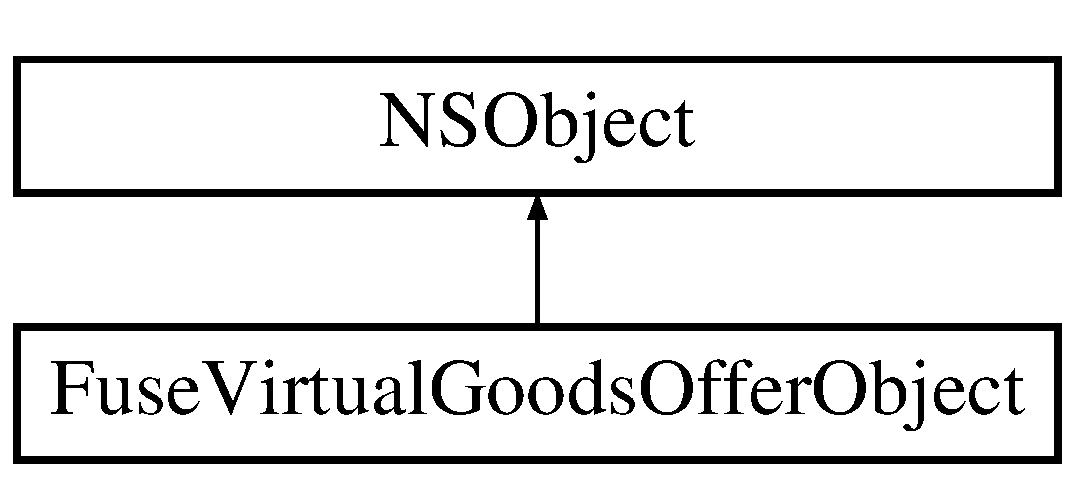
\includegraphics[height=2.000000cm]{interface_fuse_virtual_goods_offer_object}
\end{center}
\end{figure}
\subsection*{Properties}
\begin{DoxyCompactItemize}
\item 
\hypertarget{interface_fuse_virtual_goods_offer_object_a60cbcab572527ebc765b0fcbba5e1bdc}{}N\+S\+String $\ast$ {\bfseries purchase\+Currency}\label{interface_fuse_virtual_goods_offer_object_a60cbcab572527ebc765b0fcbba5e1bdc}

\item 
\hypertarget{interface_fuse_virtual_goods_offer_object_a860943b511058dbaace8344976c6000f}{}N\+S\+Number $\ast$ {\bfseries purchase\+Price}\label{interface_fuse_virtual_goods_offer_object_a860943b511058dbaace8344976c6000f}

\item 
\hypertarget{interface_fuse_virtual_goods_offer_object_afc44eae0ea1010ef7b02515dfc156e68}{}N\+S\+String $\ast$ {\bfseries item\+Name}\label{interface_fuse_virtual_goods_offer_object_afc44eae0ea1010ef7b02515dfc156e68}

\item 
\hypertarget{interface_fuse_virtual_goods_offer_object_a3eb537b8ee870de5085c035c1de25a31}{}N\+S\+Number $\ast$ {\bfseries item\+Amount}\label{interface_fuse_virtual_goods_offer_object_a3eb537b8ee870de5085c035c1de25a31}

\end{DoxyCompactItemize}


The documentation for this class was generated from the following file\+:\begin{DoxyCompactItemize}
\item 
/\+Users/buildmachine/buildmonkey/\+Fuse\+S\+D\+Ki\+O\+S-\/master/\+Code/\+Classes/\+Fuse\+S\+D\+K/Fuse\+S\+D\+K\+Definitions.\+h\end{DoxyCompactItemize}

%--- End generated contents ---

% Index
\backmatter
\newpage
\phantomsection
\clearemptydoublepage
\addcontentsline{toc}{chapter}{Index}
\printindex

\end{document}
